% cite JDemetra+

% https://en.wikipedia.org/wiki/Nowcasting_(economics)

% plot all variables +EIR with theme_bw

% Add  \cite everywhere it's needed by looking at Zotero


% ----------- Cover Master Thesis Faculty of Sciences ---------------
% This document should be compiled with pdflatex.  If you want to use
% latex to compile to dvi/ps, you have to convert the images to (e)ps
%                           -- December 2012
% -------------------------------------------------------------------
\RequirePackage{fix-cm}
\documentclass[12pt,a4paper,oneside]{book}


% ------------------------- Load packages ---------------------------
% You can eventually add these while you load other packages
% in case you want to integrate the titlepage with the rest of your thesis
% -------------------------------------------------------------------
\usepackage{graphicx,xcolor,textpos}
\usepackage{helvet}
\usepackage{multirow}

\usepackage[colorlinks=true ,citecolor=blue, linkcolor=black, urlcolor=blue]{hyperref}
\usepackage{csquotes}
\usepackage[comma]{natbib}
%\bibliographystyle{apa}
\usepackage{amsmath}
\usepackage{mathtools}

\usepackage{lipsum}

\providecommand{\keywords}[1]{\textbf{\textit{Keywords:}} #1}

%\setcounter{tocdepth}{2}% Allow only \chapter in ToC

\usepackage[Sonny]{fncychap} % chapter style

\usepackage{listings} % cite R code

\usepackage{graphicx} 
\usepackage{fancyvrb} 

\usepackage{import}
\usepackage{subfiles}

\usepackage{float}

\usepackage{dcolumn}

\usepackage{subcaption}

\usepackage{wrapfig}

\usepackage{pdflscape}

\usepackage{wasysym}

\usepackage{pgfplots}
\pgfmathdeclarefunction{gauss}{2}{%
  \pgfmathparse{1/(#2*sqrt(2*pi))*exp(-((x-#1)^2)/(2*#2^2))}%
}

\lstset{% setup listings 
        language=R,% set programming language 
        basicstyle=\small,% basic font style 
        keywordstyle=\bfseries,% keyword style 
        commentstyle=\ttfamily\itshape,% comment style 
        numbers=left,% display line numbers on the left side 
        numberstyle=\scriptsize,% use small line numbers 
        numbersep=10pt,% space between line numbers and code 
        tabsize=3,% sizes of tabs 
        showstringspaces=false,% do not replace spaces in strings by a certain character 
        captionpos=b,% positioning of the caption below 
        breaklines=true,% automatic line breaking 
        escapeinside={(*}{*)},% escaping to LaTeX 
        fancyvrb=true,% verbatim code is typset by listings 
        extendedchars=false,% prohibit extended chars (chars of codes 128--255) 
        literate={"}{{\texttt{"}}}1{<-}{{$\leftarrow$}}1{<<-}{{$\twoheadleftarrow$}}1 
        {~}{{$\sim$}}1{<=}{{$\le$}}1{>=}{{$\ge$}}1{!=}{{$\neq$}}1{^}{{$^\wedge$}}1,% item to replace, text, length of chars 
        alsoletter={.<-},% becomes a letter 
        deletekeywords={c}% remove keywords 
}

    % sections \FloatBarrier
    
\newcommand{\ImageWidth}{11cm}
\usepackage{tikz}
\usetikzlibrary{decorations.pathreplacing,positioning, arrows.meta, intersections}

\usepackage{fancyhdr}

\pagestyle{fancy}

\newenvironment{bottompar}{\par\vspace*{\fill}}{\clearpage}


\let\subsectionautorefname\sectionautorefname % if \autoref subsection -> section
\let\subsubsectionautorefname\Sectionautorefname % if \autoref subsubsection -> section

\DeclareMathOperator{\Var}{Var}
\DeclareMathOperator{\Cov}{Cov}
\DeclareMathOperator{\E}{E}
\DeclareMathOperator{\Corr}{Corr}


% ------------------------ Page settings -----------------------------
% If you change these, the cover layout will also change.  In that
% case you have to adjust the latter manually.
% --------------------------------------------------------------------

\topmargin -10mm
\textwidth 160truemm
\textheight 240truemm
\oddsidemargin 0mm
\evensidemargin 0mm

% ---------------------- textpos settings ----------------------------
% Some additional settings for the cover
% --------------------------------------------------------------------

\definecolor{green}{RGB}{172,196,0}
\definecolor{bluetitle}{RGB}{29,141,176}
\definecolor{blueaff}{RGB}{0,0,128}
\definecolor{blueline}{RGB}{82,189,236}
\setlength{\TPHorizModule}{1mm}
\setlength{\TPVertModule}{1mm}

\begin{document}

% ----------------------- Cover --------------------------------------
% Please fill in:
% - The title and subtitle (if applicable)
%         to include a formula in the title or subtitle
%         use  \form{$...$}
% - Your name
% - Your (co)supervisor, mentor (if applicable)
% - Your master
% - The academic year
% --------------------------------------------------------------------
\thispagestyle{empty}
\newcommand{\form}[1]{\scalebox{1.087}{\boldmath{#1}}}
\sffamily
%
\begin{textblock}{191}(-24,-11)
\colorbox{green}{\hspace{139mm}\ \parbox[c][18truemm]{52mm}{\textcolor{white}{FACULTY OF SCIENCE}}}
\end{textblock}
%
\begin{textblock}{70}(-18,-19)
\textblockcolour{}
\includegraphics*[height=19.8truemm]{Images/LogoKULeuven.png}
\end{textblock}
%
\begin{textblock}{160}(-6,63)
\textblockcolour{}
\vspace{-\parskip}
\flushleft
\fontsize{40}{42}\selectfont \textcolor{bluetitle}{The Variability of the Belgian Business Survey Indicator}\\[1.5mm]
\fontsize{20}{22}\selectfont Analysis and Predictive Power
\end{textblock}
%
%\begin{textblock}{82}(50,103)
%\textblockcolour{}
%\vspace{-\parskip}
%\flushleft
%\fbox{\parbox{79mm}{The background can be left blank or you can insert an image (maximum height 10 cm, width variable, mind author’s rights…). NO logos (you can use the logos inside the manuscript, but not on front or back cover). \textit{Delete this textbox.}}}
%\end{textblock}
%
\begin{textblock}{160}(8,153)
\textblockcolour{}
\vspace{-\parskip}
\flushright
\fontsize{14}{16}\selectfont \textbf{Fabrice VAN BOECKEL}
\end{textblock}
%
\begin{textblock}{70}(-6,191)
\textblockcolour{}
\vspace{-\parskip}
\flushleft
Co-Supervisor: Prof. G. Molenberghs\\[-2pt]
\textcolor{blueaff}{KU Leuven}\\[5pt]
Co-Supervisor: L. Van Belle\\[-2pt]
\textcolor{blueaff}{National Bank of Belgium}\\[5pt]
%Mentor: \textsl{(optional)}\\[-2pt]
%\textcolor{blueaff}{Affiliation \textsl{(optional)}}\\
\end{textblock}
%
\begin{textblock}{160}(8,191)
\textblockcolour{}
\vspace{-\parskip}
\flushright
Thesis presented in\\[4.5pt]
fulfillment of the requirements\\[4.5pt]
for the degree of Master of Science\\[4.5pt]
in Statistics\\
\end{textblock}
%
\begin{textblock}{160}(8,232)
\textblockcolour{}
\vspace{-\parskip}
\flushright
Academic year 2018-2019
\end{textblock}
%
\begin{textblock}{191}(-24,248)
{\color{blueline}\rule{550pt}{5.5pt}}
\end{textblock}
%
\vfill
\newpage

% In case you want to integrate the TeX-file for the titlepage
% with the rest of your thesis, you cab continue below
% ------------------------- First pages ---------------------------
% For table of contents, acknowlegments, ...
% -----------------------------------------------------------------
\rmfamily
\pagestyle{plain}


\newpage
\setcounter{page}{0}
\pagenumbering{roman}

\begin{bottompar}
\copyright Copyright by KU Leuven \\ \\
Without written permission of the promotors and the authors, it is forbidden to reproduce or adapt in any form or by any means any part of this publication. Requests for obtaining the right to reproduce or utilize parts of this publication should be addressed to KU Leuven, Faculteit Wetenschappen, Geel Huis, Kasteelpark Arenberg 11 bus 2100, 3001 Leuven (Heverlee), Telephone +32 16 32 14 01. \\
A written permission of the promotor is also required to use the methods, products, schematics and programs described in this work for industrial or commercial use, and for submitting this publication in scientific contests.
\end{bottompar}



\chapter*{Acknowledgement}

I'm grateful to my co-supervisor, Laurent Van Belle, for his guidance and his precious help.

I'm thankful to ..... that where always available to answer my questions and whose imputs during meeting where crucial to give the best direction to my work.

the National Bank of Belgium \\

Jean Palate - David ... 
and all the members of the Department of Research and Development who where always there to answer any of my questions.

Isabelle - Marc Boumon

Vanessa Baugnet - Rudi Acx 

for their time and advise during the writing of master thesis. 

I'm grateful to my co-promotor Geert Molenberghs for the guidance and feedback. Geert Loosveldt and Stephan Moens for their input during the Mid-term presentation.

Last but not least, I would like to thank all the professors of the Master of Statistics that made it possible for me to acquire the knowledge and passion of statistics, needed to write this thesis.


\begin{bottompar}
\textit{"Statistics are the heart of democracy." }

    Simeon Strunsky
\end{bottompar}


\chapter*{Abstract}


\section*{Abstract}
This Master Thesis explores the variance of the Belgian business survey. 
Several finding concerning the nature and properties of the Variance are found as the bounds and relation with the mean.

In a second part, the predictive power of the variance is examined and it's found that ...

It's also the first time that à Markov Switching model is used in this context. It was showed that ...


\section*{Samenvatting}

Deze master


\section*{Keywords}
Business Surveys - 
Business Barometer -
Trichotomous Observations -
Survey Variance - 
Survey Volatility -
Markov Switching - 



\chapter*{List of Abbreviations}

\begin{tabular}{l l}
  BSI   	& Business Survey Indicator/Barometer \\
  ECB   	& European Central Bank \\
  EIR   	& Evolution in individual Responses \\
  Eurostat & The European Statistical Office \\
  GDP   	& Gross Domestic Product \\
  NBB   	& The National Bank of Belgium \\
  NBER  	& The National Bureau of Economic Research (US) \\
  NSI   	& National Statistics Institutes \\
  Var 		& Variance \\
  Cor 		& Correlation \\
  Cov 	  & Covariance \\
  INSEE 	& \\
  YoY & Year on Year
  
\end{tabular}

\tableofcontents

\newpage
% -------------------------- Proper text --------------------------
% Introduction, chapters, ...
% -----------------------------------------------------------------
\setcounter{page}{0}
\pagenumbering{arabic}


\chapter{Introduction}

business survey indicator / business barometer / business confidence indicator

3000 participants

Panel survey

A widespread method to predict the evolution of National Economies is the survey-based Business indicator. Belgium have been collecting this indicator for more than 60 years. This long evolution 

- Talk about tradition of improving BSB

This Thesis is included in the continuity of a long tradition of papers proposing improvement and ways to add value to the Business Barometer (.......) will propose ways to add information to the Belgian Business Barometer, that could also be applied to others

Since 1968, the National Bank of Belgium publishes each month the national 



%%"A widespread method for forecasting economic macro level parameters such as GDP growth rates is surveybased indicators that contain early information in contrast to official data." (Microdata imputations and macrodata implications: Evidence from the Ifo business survey Christian Seiler Christian Heumann)

\subsubsection{Objectives}

\subsubsection{Methodology}

\subsubsection{Plan of this Paper}

Chapter 2

3

4

5





\chapter{The Business Survey Indicator}

This first chapter is a presentation of the Belgian business survey and the business survey indicator (BSI), also referred to as the business survey barometer or business confidence indicator/barometer.

First, a brief history of the business survey indicator will be presented.
The second section will discuss the sampling method while the third section will discuss the objectives of the business survey, which are (1) understanding the short term evolution by sector of the Belgian economy, (2) nowcasting and (3) the analysis of business cycles.
The next part will discuss the methodology regarding the questions and the weighting procedure(s).
In the last section of the chapter, the calculation method of the business survey indicator will be discussed.

\section{History}

The Belgian business survey celebrates this year its 65\textsuperscript{th} anniversary, since the survey was launched by the National Bank of Belgium in 1954. 
Belgium was part of the pioneers since only the United States (1930) and West Germany (1949) had a business survey at the time. 

In 1972, the results were first synthesised in an indicator.
The Business Survey Barometer started by including only the industrial sector. It was then from 1970 on, small by small enlarged to other sectors: construction, trade and services. 

Over time, several improvements of the business survey where proposed and applied (1983, 1990 and 2009). The last improvements will be discussed in detail in \autoref{section:Methodology}.

At the European level, it was in 1961 that the European Commission (EC) launched a harmonisation program of the business survey in the manufacturing industry. 
Since then, the sector coverage of the program has widened to account for the different sectors.
The harmonisation program and the large implication of the EC, make it possible to compare BSI around the European Union.
More information can be found in the "The Joint Harmonised EU Programme of Business and Consumer Surveys User Guide" \cite{european_commission_joint_2016}.

Over time, the business survey barometer got well known for being a very informative and useful indicator. 

In an article published in the Wall Street Journal titled \textit{"Euroland Discovers A Surprise Indicator: Belgian Confidence"} \citep{rhoads_euroland_1999}, the BSI is described as an important and accurate measure of the evolution of the Belgian economy. 
It also suggested that it could be a good indicator for the European Union. 
This hypothesis was test for the period of 1985-2000 in \cite{vanhaelen_belgian_2000} and the conclusion were very flattering for the BSI. 
It was shown that the BSI was indeed a leading indicator of the evolution of European economy and could quite accurately forecast turning points. 
The explanation proposed by the authors is, first of all, that the Belgian economy, in itself, had some predictive power for the European Area, since it is specialised  in  intermediate  goods and is an very open economy. 
The other potential explanation pointed out, is the high  representation  of  small and medium-sized enterprises in the business survey.

The results can't be extrapolated to the present time and some


%Today, Nowcasting is a well studied subject and very important for public and private organisation to have an as clear as possible view of the state of the economy.




\section{Sampling Method}
\label{sec:Recruitment of participants}

The Belgian business survey - as most of the business survey around the world - has the particularity of not using random sampling. 
 The selection of participants is quite complex and a lot of decision are human, never is a statistical program or a random sampling system used to select new participants.

\subsubsection{Procedure of selection}

The selection of new participants is done by waves. When the department responsible for the business survey at the NBB decides that their aren't enough participants in a specific sector anymore, the recruitment of new participants is launched.

To find the new respondents, the first step is to decided for an optimal amount of new participants needed, regarding the different stratification of the sector.
Each sector is composed of a quite advanced trees of sub-sectors, sub-sub-sectors,  and more. For example, the industry sector is divided into more than 300 sub-sectors / branches over 6 different levels. 

It could be that some sub division of a certain sector only has 1 or 2 respondents while it account for a significant part of Belgian economy, the Department of the business survey of the National Bank of Belgium will then look into which company, from that specific part of the economy, could be a good fit as new respondent of the business survey, considering it's activity, it's size, region and other characteristics.
As will be seen in \autoref{sec:Weighting procedure} and \autoref{sec:Globalisation procedure} more in detail, companies are weighted by there size (profit, number of employees, ...) and the size of the sector/branch they are part of. Those information are crucial for selecting new participants.
The procedure is quite complex and therefore contains a lot of human decisions.
 
Out of this process comes a list of potential new participants. This list is then send to the communication department that takes  contact with those potential new participants. 
Not always, but usually, a representative of the National Bank visits the new participant to explain the survey and have a contact.
As a reward for participating at the survey, the companies receive privileged information. Each month they receive access to sub-sector indicators information that aren't publicly distributed. This can give them economical information regarding there specific economical activity.

At the National Bank of Belgium, this procedure is usually referred to as prospecting, rather than selecting or sampling. Since it is mostly based on recruiting new companies that will work/collaborate with them. 

% For example, it's possible that the responsible person for the Horeca business survey, goes to  restaurant and get acquainted with the owner, sees the interest of including him in the business survey and recruits him this way. This is a less common way, the main of the recruitment happens to the process explained above.


\subsubsection{Leaving the Survey}

An important side of business survey is that people are staying as long as possible in the survey.
Ones  companies are part of the survey, they stay in it until they decide to leave, their are no participants removed from the survey by the National Bank, what can happen is that if participants don't answer for three months, contact will be taken with the company to see if they want to continue to participate.

There is a real work done by the National Bank to make sure companies answer to the survey, and stay in it.
This means that some companies are part of the survey for a very long time.
To have an idea, if we look at the survey for the industry and trace respondents back to 30 year ago (1989), we can see that today, approximately one third of the respondents where already in the survey in 1988. 

\subsubsection{Why not a problem that Random Sampling isn't used}

% The National Bank of Belgium is using random or stratified sampling for other survey. So why isn't it the case here ?

From a statistical point of view, it can seem rather problematic to draw general conclusions over a population when not  using random sampling.
Without undermining one of the most important pillars of statistics, there are two main reasons why in this case, having a non-random selection of participants is not truly problematic.

The first reason is that the sampling method used, is trying to represent as good as possible the population that it is representing. Therefore stratification is used at a quite advanced level as explained before. 
We could call this recruitment method: non-random stratification, as opposed to random stratification. Since it's not using sampling but takes into account the stratification of the population it's studying.

The second reason ,the most import one, is that the value of the business survey indicator doesn't have interest on its own. Indeed having a BSI equal to 0.5 or 0.1 don't mean much, what's important is the evolution of the indicator. If it was equal to 0.3 last month and this month it's equal to 0.5, it means that the economy is most probably growing and that we can forecast an increase of GDP over the month. On the other hand if it's now equal to 0.1, it means a decrease in economical confidence among businesses and we can anticipate a deceleration or decline of the economy over the month.


\section{Objectives of the Business Survey}
\label{section:Objective}


The main objective of the business survey barometer is to have a feeling of how the economy is now and how it will evolve in the short term.
We will here decompose the main objectives of the business survey into three subjects; (1) the direct information of the Belgian economy that can be delivered by the global and sector specific BSI, (2) Nowcasting which refers to the now and short term prediction of the economy growth and (3) the long term analysis of the business cycles and the importance of identifying turning points.

The three objectives have in common the importance, the need,  of only capturing the real evolution of the economy, without taking into account short term noise/variation as seasonal effects or bias that could erupt due to the survey method.
This will be looked into in \autoref{chap:nonresponse dropout} where seasonal effects, dropout, non-response and attrition will be discussed.


\subsection{Belgian economy and sector specific short term evolution}

%This will be less prominent in this paper, but is important to mention, each month a quite long report is done based on the BSI for each sector and sub-sector.

The business survey indicators are published at the end of each month (around the 21-25 of the month) and give a fast capture of the evolution of the Belgian economy over the past months.
The data is available on \href{http://stat.nbb.be/Index.aspx?DataSetCode=BUSSURVM&Lang=en}{stat.nbb.be} and a press release is published on \href{http://www.nbb.be/doc/dq/e/conj.htm}{nbb.be}. 
The press release contains a short summary and interpretation of the BSI followed by graphs to show the evolution of the BSI over the 4-5 last years for the sector specific and overall indicator.
The public can use those information to have a snapshot of the economy, while other indicators, as GDP or unemployment, can take a very long time before been published.

It's know ....................................




\subsection{Nowcasting}

Also called "flash" estimation, nowcasting has increasingly gain importance in the last decade (see \cite{foroni_comparison_2014}, \cite{de_antonio_liedo_nowcasting_2014}, ...).
it consists in the short term estimation of the economy, mostly the GDP.
It is a fundamental approach since the business survey indicator is published monthly while other indicator's like GDP are published quarterly.

As can be seen in \autoref{fig:timeline}, 
the lag between the observation and publication is even greater since the business survey indicator is published at the end of each month (around the 24-25\textsuperscript{th} of each month, will the GDP is published with a lag of 3 to 4 weeks and is subject to revision.

\begin{figure}[htp!]
    \centering
    \small
    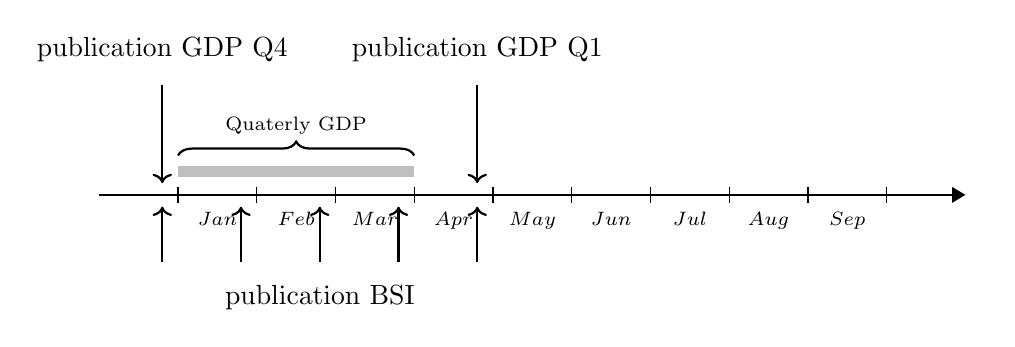
\begin{tikzpicture}
        % draw horizontal line   
        \draw[thick, -Triangle] (0,0) -- (\ImageWidth,0) node[font=\scriptsize,below left=3pt and -8pt]{ };
        % draw vertical lines
        \foreach \x in {1,...,10}
        \draw (\x cm,3pt) -- (\x cm,-3pt);
        \foreach \x/\descr in {1.5/Jan, 2.5/Feb, 3.5/Mar, 4.5/Apr, 5.5/May, 6.5/Jun, 7.5/Jul, 8.5/Aug,9.5/Sep}
        \node[font=\scriptsize, text height=1.75ex,
        text depth=.5ex] at (\x,-.3) {$\descr$};
        % colored bar up
        \foreach \x/\perccol in
        {1/100,2/75,3/25}
        \draw[lightgray, line width=4pt] 
        (\x,.3) -- +(1,0);
        % braces
        \draw [thick ,decorate,decoration={brace,amplitude=5pt}] (1,0.5)  -- +(3,0) 
               node [black,midway,above=4pt, font=\scriptsize] {Quaterly GDP};
        %\draw [thick,decorate,decoration={brace,amplitude=5pt}] (6,-.9) -- +(-1,0)
        %       node [black,midway,font=\scriptsize, below=4pt] {Publication};
        % time of publication
        \node[align=center] at (0.8,1.85) {publication GDP Q4};
        \draw [thick,->] (0.8,1.4) -- (0.8,0.15);
        \node[align=center] at (4.8,1.85) {publication GDP Q1};
        \draw [thick,->] (4.8,1.4) -- (4.8,0.15);
        \node[align=center] at (2.8,-1.3) {publication BSI};
        \draw [thick,->] (0.8,-0.85) -- (0.8,-0.15);
        \draw [thick,->] (1.8,-0.85) -- (1.8,-0.15);
        \draw [thick,->] (2.8,-0.85) -- (2.8,-0.15);
        \draw [thick,->] (3.8,-0.85) -- (3.8,-0.15);
        \draw [thick,->] (4.8,-0.85) -- (4.8,-0.15);
    \end{tikzpicture}
    \caption{Timeline of the publication of the business survey indicator (BSI) and the Gross Domestic Product (GDP)}
    \label{fig:timeline}
\end{figure}

Nowcasting got by the time a catch all word and include predictive models going from Linear models to space-space models and also including ARIMA or MIDAS and much more different models.

A good example is the State-Space model developed at the NBB to predict GDP growth \cite{de_antonio_liedo_nowcasting_2014}.

Indicators that can be used aside from the business survey are average weekly work hours, factory orders for goods, housing permits and stock prices index of consumer expectations, average weekly claims for unemployment insurance and the interest rate and more.

The advantage that the business survey indicator has over all the other indicators is that's published very fast, there is a very small gap between the companies answering the survey, and the publication of the BSI. 
Quantitative indicators take time to be collected and can be revised after been published.


\subsection{Business Cycles}
\label{sec:Business Cycles}

The theory regarding business cycles is very wide and a lot of books and articles where published on the subject. 

In 1946, \citeauthor{mitchell_measuring_1946} published the book "\textit{Measuring Business Cycles}" which is, until today, widely used as basis of business cycles theory.
In the book, business cycles are defined as recursive fluctuations, affecting macroeconomics variables.

There are a lot of variables that account the business cycles but it's commonly admitted that Growth Domestic Product (GDP) is the most important of them.

A good indicator of the growth of GDP, is Year on Year GDP that is obtained as follow

\begin{eqnarray}
   \mbox{YoY GDP} = \frac{\mbox{GDP}_t - \mbox{GDP}_{t-12}}{\mbox{GDP}_{t-12}} 
\end{eqnarray}

\autoref{fig:Business Cycle} shows a simplified version of the Business Cycles theory when using as measure GDP or YoY GDP.

\begin{figure}[htp!]
    \centering
    \small
    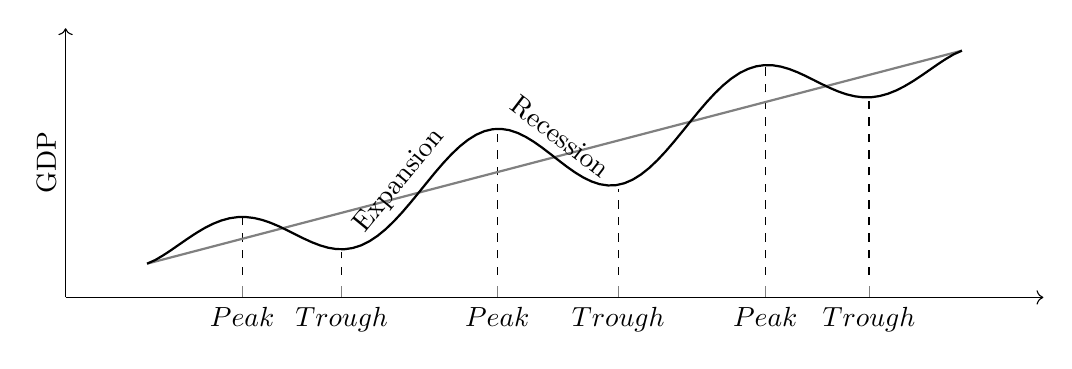
\begin{tikzpicture}
        \begin{axis}[
            domain=0:6*pi,
            samples=100,
            axis lines*=left, 
            axis line style={->},
            xtick={2.2, 4.5, 8.1, 10.9, 14.3, 16.7}, ytick=\empty,
            xticklabels = {$Peak$, $Trough$, $Peak$, $Trough$, $Peak$, $Trough$},
            width=14cm, height=5cm,
        %    xlabel={time}, 
            ylabel={GDP}
        ]       
        \addplot[mark=none, dashed] coordinates {(2.2, -1) (2.2, 4)};
        \addplot[mark=none, dashed] coordinates {(4.5, -1) (4.5, 1)}; 
        \addplot[mark=none, dashed] coordinates {(8.1, -1) (8.1, 12)}; 
        \addplot[mark=none, dashed] coordinates {(10.9, -1) (10.9, 6.6)}; 
        \addplot[mark=none, dashed] coordinates {(14.3, -1) (14.3, 17.5)}; 
        \addplot[mark=none, dashed] coordinates {(16.7, -1) (16.7, 14.9)}; 
        \addplot [thick, gray] {x};
        \addplot [thick, black] {x + 4*sin(deg(x)) * sin(deg(x/6))^0.5}
        %    node [pos=0.1, anchor=south] {Peak}
            node [pos=0.3, anchor=south, sloped] {Expansion}
            node [pos=0.49, anchor=south, sloped] {Recession}
        % Add line to show end of and ... peak and ... line
        ;
        \end{axis}
    \end{tikzpicture}
        
    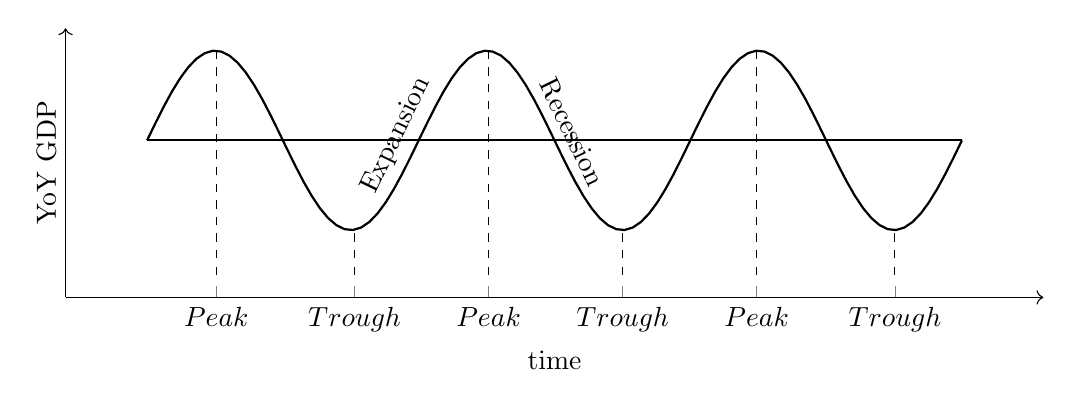
\begin{tikzpicture}
        \begin{axis}[
            domain=0:6*pi,
            samples=100,
            axis lines*=left, 
            axis line style={->},
            xtick={1.6, 4.8, 7.9, 11, 14.1, 17.3}, ytick=\empty,
            xticklabels = {$Peak$, $Trough$, $Peak$, $Trough$, $Peak$, $Trough$},
            width=14cm, height=5cm,
            xlabel={time}, 
            ylabel={YoY GDP}
        ]       
        \addplot [thick, black] {sin(deg(x))}
        %    node [pos=0.1, anchor=south] {Peak}
            node [pos=0.33, anchor=south, sloped] {Expansion}
            node [pos=0.5, anchor=south, sloped] {Recession}
        ;
        \addplot [thick, black] {0};
        \addplot[mark=none, dashed] coordinates {(1.6, -1.5) (1.6, 1)};
        \addplot[mark=none, dashed] coordinates {(4.8, -1.5) (4.8, -1)}; 
        \addplot[mark=none, dashed] coordinates {(7.9, -1.5) (7.9, 1)}; 
        \addplot[mark=none, dashed] coordinates {(11, -1.5) (11,-1)}; 
        \addplot[mark=none, dashed] coordinates {(14.1, -1.5) (14.1, 1)}; 
        \addplot[mark=none, dashed] coordinates {(17.3, -1.5) (17.3, -1)}; 
        \end{axis}
        \end{tikzpicture}
    \caption{The Business Cycle theory of GDP and Year on Year GDP}
    \label{fig:Business Cycle}
\end{figure}

\subsubsection{Duration of a Business Cycle}

A very important question considering business cycles is their duration.
\autoref{fig:Business Cycle} can give the false impression that business cycles are all of the same length, this is, in real life, not so simple.

Probably the first person to explore the duration of a business cycle was a french statistician,  \cite{juglar_crises_1862}, who set the business cycles to have a duration of 7 to 11 years.

\cite{mitchell_measuring_1946} proposed a minimum duration of 16-22 months and a maximum duration of 100-106 months (a quite large range). 

An entire book could be written about the different theories. even though business cycles are rather empirically defined than theory based.  
Therefore let put the theory aside and look into real data.
The example of the United States is interesting since the National Bureau of Economic Research (NBER) dated precisely and methodologically the turning points for the American economy. The empirical evidence that comes out of this work, is that the time from one economic peak to the next is on average 5 and a halve years for the period 1945-2009.

We can see from \autoref{fig:NBER BS}, which represent the different though and peak of business cycles identified by the NBER from 1975 to 2009, that their is no symmetry of the business cycles. Some business cycles are very short while other last more than ten years.
We can notice that periods of economical growth, usually last longer than economical decrease.


\begin{figure}[htp!]
    \centering
    \small
    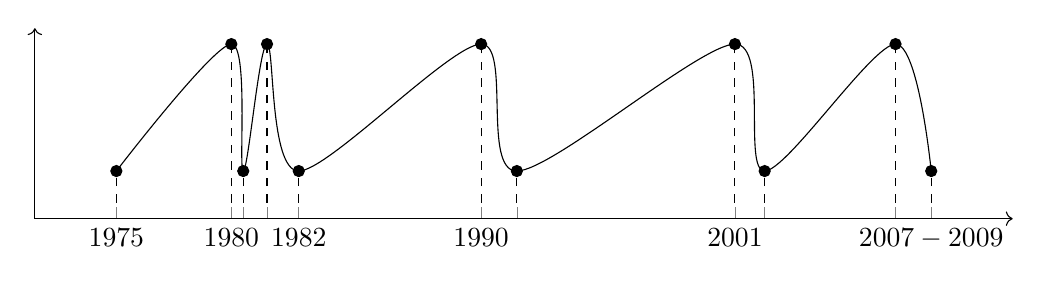
\begin{tikzpicture}
        \begin{axis}[
            domain=0:6*pi,
            samples=100,
            axis lines*=left, 
            axis line style={->},
            xtick={2103, 2161, 2167, 2179, 2195, 2287, 2305, 2415,2430, 2496, 2514}, ytick=\empty,
            xticklabels = {$1975$, $1980$,  , , $1982$, $1990$, , $2001$, , ,$2007-2009$},
            width=14cm, height=4cm
        %    xlabel={time} 
        %    ylabel={YoY GDP}
        ]       
            \addplot[smooth, mark=*,black] plot coordinates {
        	(2103,-1)
            (2161,1)	(2167,-1)
            (2179,1)	(2195,-1)
            (2287,1)	(2305,-1)
            (2415,1)	(2430,-1)
            (2496,1)	(2514,-1)
            };
        \addplot[mark=none, dashed] coordinates {(2103, -1.5) (2103, -1)};
        \addplot[mark=none, dashed] coordinates {(2161, -1.5) (2161, 1)}; 
        \addplot[mark=none, dashed] coordinates {(2167, -1.5) (2167, -1)}; 
        \addplot[mark=none, dashed] coordinates {(2179, -1.5) (2179, 1)}; 
        \addplot[mark=none, dashed] coordinates {(2195, -1.5) (2195,-1)}; 
        \addplot[mark=none, dashed] coordinates {(2287, -1.5) (2287, 1)}; 
        \addplot[mark=none, dashed] coordinates {(2305, -1.5) (2305,-1)}; 
        \addplot[mark=none, dashed] coordinates {(2415, -1.5) (2415, 1)}; 
        \addplot[mark=none, dashed] coordinates {(2430, -1.5) (2430, -1)}; 
        \addplot[mark=none, dashed] coordinates {(2496, -1.5) (2496, 1)}; 
        \addplot[mark=none, dashed] coordinates {(2514, -1.5) (2514, -1)}; 
        \end{axis}
    \end{tikzpicture}
    \caption{Business cycles from 1975 to 2009 of the American Economy according to the NBER}
    \label{fig:NBER BS}
\end{figure}


\section{Methodology of the Business Survey}
\label{section:Methodology}

%The latest large improvement of the business survey is explained in detail in \textit{"The National Bank of Belgium’s new business survey indicator"} (\citeauthor{de_greef_national_2009}).

Since 65 years of existence, the business survey ? was able to stay quite stable ?

Three main methodology revisions since the launch of the business survey, in 1983, 1990 and 2009 (see \cite{de_greef_national_2009}).

The most significant changes brought in 2009 were the amount of questions taken into the calculation of the BSI, that were reduced to 3-4 questions, depending on the sector, for more simplicity and accuracy.

Other improvements where the inclusion of services in the calculation of the global indicator and a  lighten smoothing method.


\subsection{Questionnaire}
\label{sec:Questionnaire}

The questionnaire exists in two languages, french and dutch. And can be answered by mail, email, over the phone or by fax.

The questionnaire has XX questions that can be grouped in two type of questions. 
(1) questions concerning there current production and level of activity.
(2) questions concerning there prediction, how they expect there level of activity to evolve over the next three months.
It's therefore that the business survey indicator, is also called the confidence indicator, since its a measure of how confidence companies are in the Belgian economy.


\subsubsection{Changes over time}

In this paper, the answers and results of the business survey barometer will be used since 1988. Therefore it's very important to see if the answers changed over time.

A questionnaire from 1990 was found (See Appendix \autopageref{Questionnaire1990}) and can be compared to a more recent version (See Appendix \autopageref{Questionnaire2018}).

It can be seen that the layout was modified, and that the questions phrasing changed over this long period. It was before asked in the first person while it's now phrased in the third person. Aside from those small changes, the survey kept the same questions

It would be interesting to have a closer look in the potential consequences of those changes over time. The layout, the phrasing and the method of answering can potentially have an influence on the answers. Nevertheless, since it's not the subject of this paper, we will leave this study to future research.
What we  can say is that the influence of those changes are limited since the respondents where mostly the same when the changes happened, so the interpretation they made from 
one version to the other one should have stayed quite similar.

\subsubsection{Questions taken into account for the NS975}


The first question has to be interpreted the opposite way as of the three other questions. ...



see appendix \autopageref{Questionnaire2018} for the full questionnaire


\subsection{Weighting procedure}
\label{sec:Weighting procedure}

Each company that is part of the panel of respondents, has a weight according to it's size, the profit the company is making, the capital it's owning and other characteristics. The calculation is quite complex since it's specific to each sector. For example in the industry the ...

cite working papers

According to the size of the company, measured different ways depending on the sector ........

Adapted over time, with a smoothing effect over time

\subsection{Globalisation procedure}
\label{sec:Globalisation procedure}


Based on the size of the sector in which the company is.

The National Bank of Belgium developed a quite elaborate division of the Belgian economical activity. This means that for example, the Industry is subdivided into different sub-sectors, that them self contain sub-sectors that contain sub-sectors and so on six times. All those divisions have a percentage according to the size of those subdivision inside the division.

%The globalisation procedure got quite complex over time. See the globalisation tree for the Industry survey \autopageref{fig:tree}


\newpage
\section{Calculation of the Indicator}

This section presents the method for calculating the business survey indicator. 
The calculation in itself is standard, but the different ways to write it are important for interpretation and to better understand the following chapters. 
We first present the calculation taking into account one question  unweighted and then weighted. 
After we will present how the indicator of different questions are combined together.


\subsection{Unweighted Indicator}

The calculation of the unweighted indicator for a specific question at a specific time is the mean of the responses and can be written as follow;

\begin{equation}
    E(X) = \frac{ \sum_{i=1}^n x_i}{n}
\end{equation} 

where 
$x_i$ is the answer of the respondent $i$ and can take value $-1$ (negative answer), $0$ (neutral answer) and $1$ (positive answer). 
$n$ is the number of respondents.

Since $x_i$ can only take three different values, we can decompose it into 

\begin{equation}
    E(X) = \frac{ \sum_{i=1}^n x_{+i} + \sum_{i=1}^n x_{0i} + \sum_{i=1}^n x_{-i}}{n}
\end{equation} 

\begin{equation}
    E(X) = \frac{ \sum_{i=1}^{n_+} x_{+i} + \sum_{i=1}^{n_0} x_{0i} + \sum_{i=1}^{n_-} x_{-i}}{n}
\end{equation} 


where 
$x_{+i}$, $x_{Ni}$ and $x_{-i}$ are the positive (+), neutral (N) and negative (-) answers of the respondent $i$.

Since we know that $\sum_{i=1}^n x_{0i} = 0$, we can write

\begin{equation}
    E(X) = \frac{\sum_{i=1}^n x_{+i}}{n}  + \frac{\sum_{i=1}^n x_{-i}}{n}
\end{equation} 

${\sum_{i=1}^n x_{+i}}/{n}$ is the proportion of positive answers and ${\sum_{i=1}^n x_{-i}}/{n}$ is the negative proportion of negative answer. We can write, for simplicity

\begin{equation}
    E(X) = \pi_+ - \pi_-  \label{eq: BSI Unweighted}
\end{equation}

where $\pi_+$ and $\pi_-$ are the proportion of respondents answering positive and negative to the specific question.
$\pi$ was chosen as symbol here,  since it can be interpreted as a probability: if we assume that all the respondents have the same probability giving a certain answer, $\pi$ is the probability that a respondent answers positive, negative or neutral to the question. 


\subsection{Weighted Indicator}

As described in \autoref{sec:Weighting procedure} and \autoref{sec:Globalisation procedure}, each respondent has two different weights: one according to its size, one according to the size of the sector it's part of. Those weight are then combined and we end up with a specific weight.
We have now the following equation for the indicator

\begin{equation}
    E(X) = \sum_{i=1}^n \left(\omega_i x_i \right) \quad \text{  where  } \sum_{i=1}^n \omega_i =  1
\end{equation} 

where
$x_i$ is the answer of the respondent $i$ and can take values -1, 0 and 1.
$\omega_i$ is the weight of respondent $i$. 
The weights are here standardised so there sum is equal to one.

As for the unweighted indicator, we can decompose the equation by the three possible answers with, in this case, their according weights.

\begin{equation}
    E(X) = \sum_{i=1}^n \omega_{+i} x_{+i} + \sum_{i=1}^n \omega_{0i} x_{0i} + \sum_{i=1}^n \omega_{-i} x_{-i}
 \end{equation}
and again we know that $\sum_{i=1}^n \omega_{0i} x_{0i} = 0$, so we can write

\begin{equation}
    E(X) = \sum_{i=1}^n \omega_{+i} x_{+i} + \sum_{i=1}^n \omega_{-i} x_{-i}
\end{equation} 
We also know that $x_{+i} = 1$  and $x_{-i}=-1$  
\begin{equation}
    E(X) = \sum_{i=1}^n \omega_{+i}  - \sum_{i=1}^n \omega_{-i}
\end{equation}
That will be written as follow
\begin{equation}
    E(X) = \Omega \pi_+ - \Omega \pi_- \label{eq: BSI Weighted}
\end{equation}

where $\Omega \pi_+$ and $\Omega \pi_-$ are the weighted proportion of respondents answering positive and negative. this equation will be used for the same reasons as for the unweighted indicator. 
Same explanation also works here

$\pi$ is use here also in the probabilistic way as it can also be seen as the probability that a respondent answers positive, negative or neutral ($\pi_0$) with $\pi_+ + \pi_0 + \pi_- =1$.


From \autoref{eq: BSI Unweighted} and \autoref{eq: BSI Weighted} it can be seen that the weighted and unweighted indicators are bounded between -1 and 1. In the two cases, the indicator is the smallest if everyone has a negative answer, and is the largest when every answer is positive.

\subsection{Take different questions into account}

The previous calculations where specific to each question. The published indicators are usually taking different survey questions into account. For example the Industry indicator that we will be interested in is composed of four questions that have all the same weight:

\begin{equation}
    \mbox{Industry business indicator}\ = \frac{E(X_{Q1}) + E(X_{Q2}) + E(X_{Q3}) + E(X_{Q4})}{4}
\end{equation}

where 
$E(X_{Q1})$, $E(X_{Q2})$, $E(X_{Q3})$ and $E(X_{Q4})$ are the different averages for question 18, 27, 32 and 33 (can be weighted or unweighted)

can also been seen as the mean of the answers for each participant at each period then combined together

\begin{equation}
    \mbox{Industry business survey indicator}\ = \frac{\sum_{i=1}^n \left(x_{i Q1} + x_{i Q2} + x_{i Q3} + x_{i Q4} \right)}{4n}
\end{equation}

\begin{equation}
    \mbox{Industry BSI}\ = \frac{\pi_{Q1+} + \pi_{Q2+} + \pi_{Q3+} + \pi_{Q4+} - \pi_{Q1-} - \pi_{Q2-} - \pi_{Q3-} - \pi_{Q4-} }{4}
\end{equation}


\begin{eqnarray}
    \mbox{ Weighted Industry BSI}\ &=& 1/4 ( \pi_{Q1+} + \Omega \pi_{Q2+} + \Omega \pi_{Q3+} + \Omega \pi_{Q4+} \\
    && - \Omega \pi_{Q1-} - \Omega \pi_{Q2-} - \Omega \pi_{Q3-} - \Omega \pi_{Q4-} \Large) 
\end{eqnarray}

Generalisation !


\chapter{The Variance of the Indicator}

The variance is, with the mean, one of the first tool for Statisticians to study a certain variable. Next to the mean, that is the average value of a certain variable, the variance is the measure of the dispersion. 
In the context of the business survey, the variance haven't been used much, while it can be seen as "how much people agree", an important information that we can extract from the survey.

The variance will be interpreted as to what level respondents agree about the state of the Belgian economy.

% A small comment can be written regarding the difference between the variance and sampling error. The idea here is not the study accuracy or ... but rather to find new information hidden in the survey.

This chapter will present the calculation of the variance of the unweighted and weighted indicator.
It will then look into the properties and specificities of the variance of the business survey indicator.

% As done for the indicator, two different variances will be take into account here, the weighted and the unweighted variance of the indicator.


\section{Variance of the Unweighted Indicator}

% \cite{alcaniz_calculation_2006}

\nocite{alcaniz_calculation_2006}

The formula of the variance can be written as 
\begin{eqnarray}
         \Var(X) &=& E \left[ \left(X-E(X) \right)^2 \right] =  E\left( X^2\right) - E\left( X\right)^2
\end{eqnarray}

In the case of one question of the business survey indicator, we can write and develop the equation as follow

\begin{eqnarray}
\Var(X) &=&  E\left( X^2\right) - E\left( X\right)^2 \nonumber \\ \nonumber \\
    &=& \left( \frac{\sum_{i=1}^n x_{-i}^2}{n} \right) + \left( \frac{\sum_{i=1}^n x_{0i}^2}{n} \right) + \left( \frac{\sum_{i=1}^n x_{+i}^2}{n} \right) - E(X)^2 \\ \nonumber 
\end{eqnarray}


The positive and negative answers take value -1 and 1, which means that $x_{+i}^2 = x_{+i}$, $x_{-i}^2 = |x_{-i}|$. We also know that $\left( \frac{\sum_{i=1}^n x_{Ni}^2}{n} \right) = 0$. 
With this information, we can further simplify the equation;

\begin{eqnarray}
	\Var(X) &=& \pi_+ + \pi_- - E ( X )^2 \label{var1} \\ \nonumber
\end{eqnarray}

In other words, the variance of the BSI is equal to the sum of the proportion of positive and negative answers, minus the squared indicator. \\
We can also replace $\E(X)$  by $\pi_+ - \pi_-$, and/or $\pi_+ + \pi_-$ by $ 1 - \pi_0$ (since $\pi_+ \pi_0 + \pi_- = 1$).
Which means that we have several different ways to write the previous equation;

\begin{eqnarray}
\Var(X) &=& \pi_+ + \pi_- - E ( X )^2  \nonumber \\
        &=& \pi_+ + \pi_- - ( \pi_+ - \pi_- )^2 \label{var2} \\
	    &=& 1 - \pi_0 - E(X)^2 \label{var3}
\end{eqnarray}




\section{Variance of the Weighted Indicator}

We can now do the same for the weighted indicator. The equation is very similar as for the variance of the unweighted variance;



\begin{eqnarray}
\Var(X) &=&  E\left( X^2\right) - E\left( X\right)^2 \nonumber \\ \nonumber \\
    &=& \sum_{i=1}^n \omega_i x_{+i}^2 + \sum_{i=1}^n \omega_i x_{0i}^2  + \sum_{i=1}^n \omega_i x_{-i}^2 - E(X)^2 \nonumber \\
\end{eqnarray}

We can here, as we did for the indicator, take into account weighted proportion and write the equation the same way as for the unweighted variance but in this case, by taking the weighted proportions. Again the variance can be written in different ways, depending on the interpretation that fits best;

\begin{eqnarray}
\Var(X) &=& \Omega \pi_+ + \Omega \pi_- - ( \Omega \pi_+ - \Omega \pi_- )^2 \\
	&=& \Omega \pi_+ + \Omega \pi_- - E ( X )^2 \\
	&=& 1 - \Omega \pi_{0} - E(X)^2
\end{eqnarray}


\section{Properties}

\begin{figure}[hbt!]
    \centering
    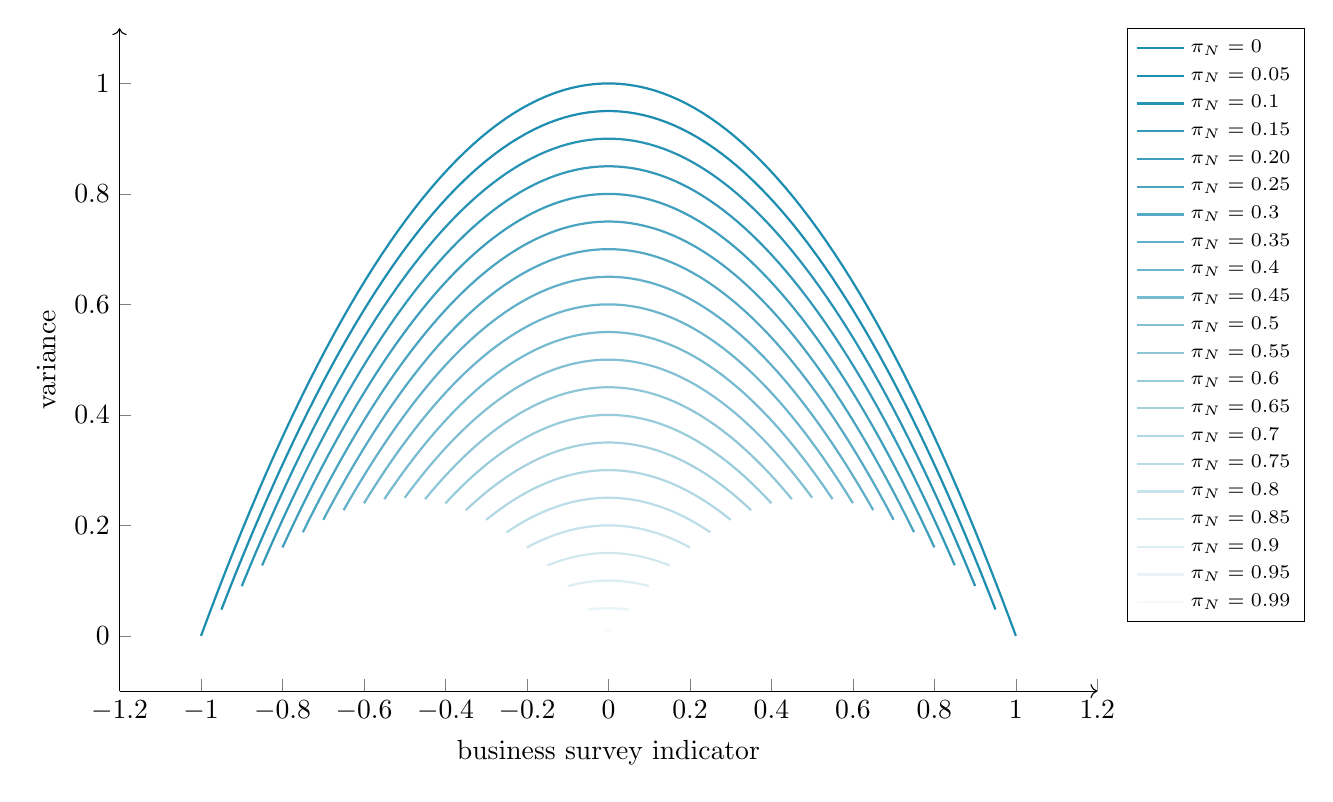
\begin{tikzpicture}
    \tikzset{
      legendmatrix/.style={% style for legends
        draw,% draw a border for the legend
        outer sep=.3333em,% additional space to the axis label
        nodes={rotate=90,anchor=base west,outer sep=0pt},% rotate the nodes inside the matrix
        /pgfplots/every crossref picture/.append style={yshift=.75ex}% rotate the legend images
      }
    }
    \begin{axis}[
        domain=-1:1,
        samples=100,
        axis lines*=left, 
        axis line style={->},
        width=14cm, height=10cm,
        xlabel={business survey indicator}, ylabel={variance},
    legend pos= outer north east, legend cell align=left,
     legend style={font=\scriptsize}
     ]       
    \addplot [thick, bluetitle!100, domain = -1:1] {1 - x^2};
    \addplot [thick, bluetitle!100, domain = -0.95:0.95] {1 - 0.05 - x^2};
    \addplot [thick, bluetitle!95, domain = -0.9:0.9] {1 - 0.1 - x^2};
    \addplot [thick, bluetitle!90, domain = -0.85:0.85] {1 - 0.15 - x^2};
    \addplot [thick, bluetitle!85, domain = -0.8:0.8] {1 - 0.2 - x^2};
    \addplot [thick, bluetitle!80, domain = -0.75:0.75] {1 - 0.25 - x^2};
    \addplot [thick, bluetitle!75, domain = -0.7:0.7] {1 - 0.3 - x^2};
    \addplot [thick, bluetitle!70, domain = -0.65:0.65] {1 - 0.35 - x^2};
    \addplot [thick, bluetitle!65, domain = -0.6:0.6] {1 - 0.4 - x^2};
    \addplot [thick, bluetitle!60, domain = -0.55:0.55] {1 - 0.45 - x^2};
    \addplot [thick, bluetitle!55, domain = -0.5:0.5] {1 - 0.5 - x^2};
    \addplot [thick, bluetitle!50, domain = -0.45:0.45] {1 - 0.55 - x^2};
    \addplot [thick, bluetitle!45, domain = -0.4:0.4] {1 - 0.6 - x^2};
    \addplot [thick, bluetitle!40, domain = -0.35:0.35] {1 - 0.65 - x^2};
    \addplot [thick, bluetitle!35, domain = -0.3:0.3] {1 - 0.7 - x^2};
    \addplot [thick, bluetitle!30, domain = -0.25:0.25] {1 - 0.75 - x^2};
    \addplot [thick, bluetitle!25, domain = -0.2:0.2] {1 - 0.8 - x^2};
    \addplot [thick, bluetitle!20, domain = -0.15:0.15] {1 - 0.85 - x^2};
    \addplot [thick, bluetitle!15, domain = -0.1:0.1] {1 - 0.9 - x^2};
    \addplot [thick, bluetitle!10, domain = -0.05:0.05] {1 - 0.95 - x^2};
    \addplot [thick, bluetitle!05, domain = -0.01:0.01] {1 - 0.99 - x^2};
 %    \addplot [thick, black, domain = -1:0] { - ((x+0.5)^2) + 0.25};
 %    \addplot [thick, black, domain = 0:1] { - ((x-0.5)^2) + 0.25};
%     \addplot [thick, black, domain = -1:0] {-x-x^2};
%     \addplot [thick, black, domain = 0:1] {x-x^2};
%     \addplot [thick, black, domain = -1:1] {(x^2)*(-y)-(y^2)/2 + y};    
	\addlegendentry{$\pi_N = 0$}
    \addlegendentry{$\pi_N = 0.05$}
    \addlegendentry{$\pi_N = 0.1$}
    \addlegendentry{$\pi_N = 0.15$}
    \addlegendentry{$\pi_N = 0.20$}
    \addlegendentry{$\pi_N = 0.25$}
    \addlegendentry{$\pi_N = 0.3$}
    \addlegendentry{$\pi_N = 0.35$}
    \addlegendentry{$\pi_N = 0.4$}
    \addlegendentry{$\pi_N = 0.45$}
    \addlegendentry{$\pi_N = 0.5$}
    \addlegendentry{$\pi_N = 0.55$}
    \addlegendentry{$\pi_N = 0.6$}
    \addlegendentry{$\pi_N = 0.65$}
    \addlegendentry{$\pi_N = 0.7$}
    \addlegendentry{$\pi_N = 0.75$}
    \addlegendentry{$\pi_N = 0.8$}
    \addlegendentry{$\pi_N = 0.85$}
    \addlegendentry{$\pi_N = 0.9$}
    \addlegendentry{$\pi_N = 0.95$}
    \addlegendentry{$\pi_N = 0.99$}
    \end{axis}
    \end{tikzpicture}
    \caption{Plot of the possible values of the business survey indicator (X axis) and variance (Y axis) for different values of $\pi_N$ }
    \label{fig:var properties}
\end{figure}


Based on the previous development of the equation of the variance of the indicator, we can make some observations.

First of all, the variance is bounded between 0 and 1. 
A variance can't be negative since it's a sum of squares, so the lower bound shouldn't surprise anyone. On the other hand, the upper bound is more unusual. The most interesting approach is to take  \autoref{var3} and see that $\pi_0$ and $\E(X)^2$ can only take positive values. Since both the variables have a minus sign in front of them, to have the highest result they should both be equal to zero. 
This means that the highest variance, $\Var(X)=1$, is obtained when no respondent answer "neutral" and the BSI is equal to 0, in other words, half of the respondents answer "positive" while the other half answer "negative". 
On the other hand, the variance will be equal to zero if all the participant answer the same, that's "negative", "neutral" or "positive".

Another approach to better understand the variance of the business survey barometer, is to plot the different possible values of $\Var(X)$, $\pi_0$ and $\E(X)$ from \autoref{var3}. The results can be seen in \autoref{fig:var properties}.

Their are different observations that can be done from the plot;
(1) there is a specific upper and lower bound for each BSI

upper bound : 
\begin{equation}
    \Var(X) = 1 - 0 - \E(X)^2
\end{equation}

lower bound : 
\begin{eqnarray}
\Var(X) &=& X - X^2 \quad \text{where } \Var(X) \text{ is between -1 and 0} \\
    &=& - (\E(X) + 0,5)^2 + 0,25 
\end{eqnarray}

\begin{eqnarray}
    \Var(X) &=& - X - X^2 \quad \text{where } \Var(X) \text{ is between 0 and 1} \\
        &=&  - (\E(X) - 0,5)^2 + 0,25
\end{eqnarray}
    

\section{Take different questions into account}

As already seen, the published indicator take different questions into account. 
The combination of the variance of different questions is slightly more complex than the combination of different indicators since the questions are correlated, which means that covariance has to be taken into account.

The formula to combine different variances is the following

\begin{equation}
\Var \left(\sum_{i=1}^{n} X_{i}\right) = \sum_{i=1}^{n} \sum_{j=1}^{n} \Cov\left(X_{i}, X_{j}\right)
= \sum_{i=1}^{n} \Var\left(X_{i}\right)+2 \sum_{1 \leq i<j \leq n} \Cov\left(X_{i}, X_{j}\right)
\end{equation}

In the case of combining the variances of four different questions of the business survey, we have the following equation

\begin{eqnarray}
    \Var \left(\frac{X_{Q1} + X_{Q2} + X_{Q3} + X_{Q4}}{4} \right) &=& \frac{1}{16} \large[ \Var(X_{Q1}) + \Var(X_{Q2}) + \Var(X_{Q3}) + \Var(X_{Q4}) \nonumber \\
    && + 2 \Cov (X_{Q1},X_{Q2}) + 2 \Cov (X_{Q1},X_{Q3}) + 2 \Cov (X_{Q1},X_{Q4}) \nonumber \\
    &&  + 2 \Cov (X_{Q2},X_{Q3}) + 2 \Cov (X_{Q2},X_{Q4}) + 2 \Cov (X_{Q3},X_{Q4}) \large] \nonumber
\end{eqnarray}

The complexity of the formula encourage to rather calculate the indicator (taking all the questions into account), and then calculate the variance of that indicator, we can write it as follow

\begin{eqnarray}
    \Var \left(\frac{X_{Q1} + X_{Q2} + X_{Q3} + X_{Q4}}{4} \right) 
    &=& \frac{1}{16} \Var \left(\frac{\sum_{i=1}^n \left(x_{i Q1} + x_{i Q2} + x_{i Q3} + x_{i Q4} \right)}{n} \right) \nonumber \\
    &=& \frac{1}{16} \Var \left(\pi_{1+} + \pi_{2+} + \pi_{3+} + \pi_{4+} - \pi_{1-} - \pi_{2-} - \pi_{3-} - \pi_{4-}  \right) \nonumber \\
 %   &=& \frac{1}{16} \Var \left(\pi_{1+} + \pi_{2+} + \pi_{3+} + \pi_{4+} - \pi_{1-} - \pi_{2-} - \pi_{3-} - \pi_{4-} \right) \nonumber \\
\end{eqnarray}

The generalisation of the previous equation can be written as follow

\begin{eqnarray}
    \Var \left(\frac{X_{Q1} + X_{Q2} + \ldots + X_{Qn}}{n_Q} \right) 
    &=& \frac{1}{n_Q^2} \Var \left(\frac{\sum_{i=1}^n \left(x_{i Q1} + x_{i Q2} + ... + x_{i Qn} \right)}{n} \right) \nonumber \\
    &=& \frac{1}{n_Q^2} \Var \left(\pi_{1+} + \pi_{2+} + \ldots + \pi_{n+} - \pi_{1-} - \pi_{2-} - \ldots - \pi_{n-} \right) \nonumber \\
\end{eqnarray}

\chapter{The Indicator of the Evolution of Individual Responses}

In the same logic as for the variance, a proposition is done here of a way to extract more information out of the business survey. 
As explained in the first chapter, the business survey is answered by the same companies over time, there are some new recruits and companies leaving the survey, but the survey can be referred to as a panel survey.
Is it possible to have more information by taking taking the evolution of the individual respondents into account ? 

This chapter will address this question by applying a method proposed by \cite{caron_estimation_1996} that, by taking all the individual evolution of responses into account, offers a method to calculate an indicator that will be called the indicator of the evolution of individual responses (EIR).

First the calculation will be described for the and the intuition will be developed .


We will here describe and develop this indicator, that we will call Evolution of individual Responses (EIR).
It can be understood as the indicator of the changes in individual answers between t-1 and t.

As for the variance, The EIR has no ambition of replacing the BSI but rather to propose an addition information.

\subsubsection{Explanation}

To understand this new indicator, it's important to see that if we take only one period into account, there are three different possibilities of answers; "negative", "neutral" and "positive". 
When we take two periods into account, a month (t) and the previous one (t-1) for example, there are nine possible situations as represented in \autoref{tab:EIR explanation}. 
We can again see that $\pi$ is used since we will speak about proportions and probabilities of been in a certain group, as done before.

\begin{table}[H]
    \centering
    \begin{tabular}{r | r | c c c | }
    \multicolumn{1}{r}{} & \multicolumn{1}{r}{} &	\multicolumn{3}{c}{$t$} \\ \cline{3-5}
    \multicolumn{1}{r}{} & 		& \textbf{-} & \textbf{0} & \textbf{+} \\ \cline{2-5}
    		&    \textbf{-} & $z_{i--}$	& $z_{i-0}$	& $z_{i-+}$ \\ 
    $t-1$ & \textbf{0} & $z_{i0-}$	& $z_{i00}$	& $z_{i0+}$	\\
    		&    \textbf{+} & $z_{i+-}$	& $z_{i+0}$	& $z_{i++}$ \\ \cline{2-5}
    \end{tabular}
    \caption{Possible observation when taking t and t-1 into account}
    \label{tab:EIR explanation}
\end{table}{}

The same as for the BSI, the EIR take different values. In the case of the BSI, if the answer was negative, it would take value "-1", neutral it would take value "0" and positive it would take value "1".

The EIR defers in the sens that it's a measure of change, so if the answer of a certain respondent is the same at a certain time and at the previous survey, $x=0$. 
On the other hand, if a certain participant changes his answer for a more positive answer it will take value 1, except if it's a radical change from a "negative" to a "positive" answer, then it will take value 2.
Same the other way around, if it decreases it will take value -1, except for a radical change from "positive" to "negative".
We will here use $z$ rather than $x$ to make a clear distinction between the BSI and the EIR.

A summary to better understand this new indicator can be seen in \autoref{tab:values EIR}. 

\begin{table}[H]
    \centering
    \begin{tabular}{r | r | c c c | }
    \multicolumn{1}{r}{} & \multicolumn{1}{r}{} &	\multicolumn{3}{c}{$t$} \\ \cline{3-5}
    \multicolumn{1}{r}{} & 		& \textbf{-} & \textbf{0} & \textbf{+} \\ \cline{2-5}
   		&    \textbf{-} & $z_{i--}=0$	& $z_{i-0}=1$	& $z_{i-+}=2$ \\ 
    $t-1$ & \textbf{0}  & $z_{i0-}=-1$	& $z_{i00}=0$	& $z_{i0+}=1$	\\
    		& \textbf{+}& $z_{i+-}=-2$	& $z_{i+0}=-1$	& $z_{i++}=0$ \\ \cline{2-5}
\end{tabular}
    \caption{Value given at each type of $z_i$}
    \label{tab:values EIR}
\end{table}{}

\section{Indicator of the Unweighted Evolution of Individual Responses}

% \begin{equation}
%    \pi_{++} + \pi_{+0} + \pi_{+-} + \pi_{0+} + \pi_{00} + \pi_{0-} + \pi_{-+} + \pi_{-0} + \pi_{--} = 1
% \end{equation}

The Indicator of the evolution of the individual responses can be obtained by taking the mean of the values, as defined in \autoref{tab:values EIR}, the formula is then

\begin{eqnarray}
    \E(Z) &=&  \frac{ \sum_{i=1}^n z_i}{n} \\ \nonumber \\
        &=& \left( \frac{ \sum_{i=1}^n z_{--i}}{n} \right)
     + \left( \frac{\sum_{i=1}^n z_{-0i} }{n} \right)
    + \left( \frac{\sum_{i=1}^n z_{-+i}}{n} \right)
    + \left( \frac{\sum_{i=1}^n z_{0-i} }{n} \right)
    + \left( \frac{\sum_{i=1}^n z_{00i} }{n} \right) \nonumber  \\
    &&  + \left( \frac{\sum_{i=1}^n z_{0+i}}{n} \right)
    + \left( \frac{\sum_{i=1}^n z_{+-i} }{n} \right)
    + \left( \frac{\sum_{i=1}^n z_{+0i} }{n} \right)
    + \left( \frac{\sum_{i=1}^n z_{+-i}}{n} \right)
\end{eqnarray}

As for the indicator, we will now move from individual responses, to proportions, that can be seen in \autoref{tab:EIR proportions}.

\begin{table}[H]
    \centering
    \begin{tabular}{r | r | c c c | }
    \multicolumn{1}{r}{} & \multicolumn{1}{r}{} &	\multicolumn{3}{c}{$t$} \\ \cline{3-5}
    \multicolumn{1}{r}{} & 		& \textbf{-} & \textbf{0} & \textbf{+} \\ \cline{2-5}
    		&    \textbf{-} & $\pi_{--}$	& $\pi_{-0}$	& $\pi_{-+}$ \\ 
    $t-1$ & \textbf{0} & $\pi_{0-}$	& $\pi_{00}$	& $\pi_{0+}$	\\
    		&    \textbf{+} & $\pi_{+-}$	& $\pi_{+0}$	& $\pi_{++}$ \\ \cline{2-5}
    \end{tabular}    
    \caption{Possible observation when taking t and t-1 into account}
    \label{tab:EIR proportions}
\end{table}

The EIR can now be calculated with the following expression after taking out $\pi_{--}$, $\pi_{00}$ and $\pi_{++}$ since $z_{--}$, $z_{00}$ and $z_{++}$ have value zero.

\begin{equation}
    \E(Z) = \pi_{0+} + \pi_{-0} - \pi_{+0} - \pi_{0-} +2\pi_{-+} -2\pi_{+-} 
\end{equation}

where $\pi$ is the proportion/probability of respondent answering negative(-), neutral (0) and positive (+) at $t-1$ and $t$. 


\subsubsection{?Interpretation}


\section{Indicator of the Weighted Evolution of Individual Responses}

bla bla bla

\section{Take different questions into account}

bla bla bla

\section{Generalisation for n time frames}

Changes in the economy are usually taking several months to influence all the companies. There can be some lag of effects on for example larger companies, of a very specific sector.
The idea of only taking a certain month and the previous month can seems non-sufficient, it's relevant to take a larger period into account. 

Different methods where explored to take more than two periods into account, but it was found as been flawed and very complex to interpret.
We rather propose here a simple generalisation; use t-n rather than t-1. You compare then that period t-n with the the answer at t, without taking the between answers into account.

\subsubsection{t-n vs t}

come up to the same except that you use a larger period into account


\chapter{The Variance of the Evolution of Individual Responses} \label{Chapter:Var Z}

The new indicator, the evolution of individual responses, also has a variance that has some interpretation interest. 
While the EIR is a measure of in which direction companies change there answer, the variance of the EIR can be understood as the measure of changes in answers. Therefore the Var(EIR) can be seen as the volatility of the indicator, in the sens that the variance of the EIR account for the dispersion of the difference in answers over a two times period.

\subsubsection{difference var(BSI) \& var(EIR)}

That we will also call the volatility of the indicator, in the sens that the variance of the evolution of the indicator account for the dispersion of the difference in answers over a two times period.

% In this case, the highest the variance of EIR, will be obtained when half of the companies went from a negative answer to a positive answer and the other half did the opposite and changed from a positive answer at t-1 to a negative answer at t. 

The idea is that this variance of EIR is complementary to the estimation of Z since they have two very interesting but different interpretations.
Further interpretation will be 

\section{Variance of the Unweighted Evolution of Individual Responses}



%\begin{equation}
%    \pi_{++} + \pi_{+0} + \pi_{+-} + \pi_{0+} + \pi_{00} + \pi_{0-} + \pi_{-+} + \pi_{-0} + \pi_{--} = 1 
%\end{equation}

\begin{eqnarray}
Var(Z) &=& \pi_{0+} + \pi_{-0} + \pi_{+0} + \pi_{0-} +4\pi_{-+} +4\pi_{+-} \nonumber \nonumber \\ 
&&	- (\pi_{0+} + \pi_{-0} - \pi_{+0} - \pi_{0-} +2\pi_{-+} -2\pi_{+-})^2 \nonumber \\
&=& \pi_{0+} + \pi_{-0} + \pi_{+0} + \pi_{0-} +4\pi_{-+} +4\pi_{+-} - E(Z)^2 \nonumber \\
&=& 1 - \pi_{++} - \pi_{00} - \pi_{--} + 3\pi_{+-} + 3\pi_{-+} - E(Z)^2
\end{eqnarray}

\begin{eqnarray*}
Var(Z) &=& 
\left(\begin{tabular}{r|r r r}
    			& \textbf{-} & \textbf{0} & \textbf{+} \\\hline
    \textbf{-} 	& 0		& +1	& +4	\\
    \textbf{0} 	& +1	& 0		& +1	\\
    \textbf{+} 	& +4	& +1	& 0		\\
\end{tabular} \right)
- \left(
\begin{tabular}{r|r r r}
    			& \textbf{-} & \textbf{0} & \textbf{+} \\\hline
    \textbf{-} 	& 0		& +1	& +2	\\
    \textbf{0} 	& -1	& 0		& +1	\\
    \textbf{+} 	& -2	& -1	& 0		\\
\end{tabular}
\right)^2  \\
&=& \left( \begin{tabular}{r|r r r}
    			& \textbf{-} & \textbf{0} & \textbf{+} \\\hline
    \textbf{-} 	& 0		& +1	& +4	\\
    \textbf{0} 	& +1	& 0		& +1	\\
    \textbf{+} 	& +4	& +1	& 0		\\
\end{tabular} \right)
- \left(E(Z)\right)^2 	\\
&=& 1 +  \left(\begin{tabular}{r|r r r}
    			& \textbf{-} & \textbf{0} & \textbf{+} \\\hline
    \textbf{-} 	& -1	& 0		& +3	\\
    \textbf{0} 	& 0		& -1	& 0	\\
    \textbf{+} 	& +3	& 0		& -1		\\
\end{tabular} \right)
 - \left(E(Z)\right)^2	\\
\end{eqnarray*}







\section{Variance of the Weighted EIR}


\section{Properties}

quite similar to Var(BSI)


\subsubsection{Property 1: the variance of Z is bounded between -1 and 1}


\subsubsection{Property 2: }

\section{Take different questions into account}




\chapter{Non-Response, Dropout, Attrition and Seasonal Effects}
\label{chap:nonresponse dropout}

Before we model the data, it's important to look at the different effects that could mislead the outcome of the analysis. After exploring the data and doing a literature review, there are four effects that could mislead the results. Three are due to the survey and one to external effects, seasonal effects. We will first look into the three survey based issues; non-response, dropout and attrition, and will then explain the seasonal correction applied to the data.


\begin{table}[!htbp] \centering 
  \caption{Correlation Between Time and different variables} 
  \label{tab:corr time} 
\begin{tabular}{@{\extracolsep{5pt}} cccccccc} 
\\[-1.8ex]\hline 
\hline \\[-1.8ex] 
  & GDP & YoY GDP & BSI & Var & Z\_I & Var\_Z\_I \\ 
\hline \\[-1.8ex] 
Time & $-0.223$ & $-0.352$ & $0.148$ & $-0.775$ & $0.060$ & $-0.728$ \\ 
\hline \\[-1.8ex] 
\end{tabular} 
\end{table}



\section{Non-Response}

Non-response is one of the most studied issues in Surveying. Indeed it is a large issue

two ways 
- non participation to the survey
- participating but not answering 

- non participation to the survey
has already been mentioned before, the stratified procedure should avoid as much as possible it, and in the main time, since the importance is the evolution of the Indicator.

- participating but not answering 
 solved by the National Bank by filling the non-answering by the previous response of the participant. 
The response rate is usually around 95\% for the business survey. We could from there say that non-response is not very important. 
Before concluding it, since the mean study is the evolution rather than the indicator in it self, we plotted the non-response with the evolution of the Year on Year GDP to see if there seems to be a relation between the two. For example we could expect more or less non-response during crises or in certain economy situations. Since the main interest of the BSI is to explain Business cycles,
this could be an issue.

plot non-response



\section{Dropout and Attrition}

Those two issues are related to the structure and organisation of the survey. As explain in \autoref{sec:Recruitment of participants}, ones participants are recruited to participate in the business survey, they stay as long as they want. This brings to major potential issues: dropout and attrition

\subsection{Dropout}

Participants leaving the survey, are they different from 

The National Bank doesn't keep track from reasons why participants leave the survey. From discussions with the employees at the NBB, the two mean reasons are (1) the company going bankrupt, acquired or merged and (2) the responsible person at the company leaves his job there and the new responsible person doesn't see the interest in participating anymore.
This is an issue, since it means that it's a certain type of profiles that leave the survey. If this type of profile have a different opinion or respond differently than the remaining companies this will create bias. 

This is the case

It could be argued that the bias is very diffused due to the small amount of companies leaving the survey each month. Again the fact that the evolution is important, means that we have a very small bias for each month (if we take a long period into account then the bias become larger) we are only comparing month to month evolution, and when the business survey is published, the 3-4 last year are showed.

It's not the subject of this work, so will not dive more into this bias, but we would recommend to have a closer look into this.

\subsection{Attrition}
Attrition, also called Panel Conditioning, is present when participants change there behaviour between different rounds of sampling. 
A very interesting master thesis was done about the Belgian Labour Force Survey, where attrition was found to be significant \cite{priyana_hardjawidjaksana_investigating_2019}. 
The Belgian Labour Force Survey was convenient to test for attrition, since it's a survey where respondents reply four times to the same survey with a lag of six months.

In the case of the Business Industry Survey it's a harder to test for it since we have only two major periods of recruitment for the period at interest (1988 - 2018); in the early 1900 and between XXX and XXXX with some company 

plot of the amount of recruited over time

Two possible indicators to show the presence of Attrition, is the correlation between time and variance(BSI) and the correlation between time and variance(EIR).

corr(time,var(BSI))

corr(time,var(EIR))



Non parametric test \cite{das_nonparametric_2011}


\section{Seasonal Effects and Correction}
The National Bank, before publishing the business survey indicator, applies a X11 seasonal correction.

The literature about seasonal effects is very rich and variate


\subsubsection{JDemetra+}

% most widely used and recommended -12-ARIMA2/X-13ARIMA-SEATS3 developed at the U.S. Census Bureau and TRAMO/SEATS4 developed by Victor Gómez and Agustín Maravall, from the Bank of Spain. Both methods are divided into two main parts. The first part is called pre-adjustment and removes deterministic effects from the series by means of a regression model with ARIMA noise. The second part is the decomposition of the time series to estimate and re-move a seasonal component. TRAMO/SEATS and X-12-ARIMA/X-13ARIMA-SEATS use a very similar approach in the first part to estimate the same model on the processing step, but they differ completely in the decomposition step. Therefore, comparing results from decomposition is often difficult. Furthermore, their diagnostics focus on different aspects and their outputs take completely different forms.  

The department of Research and development of the NBB developed JDemetra+ and has since been recommended by the European Central Bank (ECB) and the European Statistical Office (Eurostat) for all National Statistics Institutes (NSI) of the European Union. 


Test for seasonality where done with JDemetra (see appendix \autopageref{sec:test for seasonality}) and it was concluded that there was seasonal effect for each of the variables at hand.

\subsubsection{Seasonality Tests}

bla bla

\begin{table}[H]
    \centering \footnotesize
    \begin{tabular}{l|c|c|c|c|c|c|c|c}
\textbf{Seasonality Test} & BSI & Var(BSI) & EIR & Var(EIR) & EIR2 & Var(EIR2) & EIR3 & Var(EIR3) \\ \hline
Auto-correlations at seasonal lags& YES & YES & YES & YES & YES & YES & YES & YES \\
Friedman (non parametric)       & YES   & YES & YES & YES & YES & YES & YES & YES \\
Kruskall-Wallis (non parametric)& YES   & YES & YES & YES & YES & YES & YES & YES \\
Spectral peaks                  & YES   & YES & YES & ? & YES & ? & YES & YES \\
Periodogram                     & YES   & YES & YES & YES & YES & YES & YES & YES \\
Seasonal dummies                & YES   & YES & YES & YES & YES & YES & YES & YES \\
Seasonal dummies (AMI)          & YES   & YES & YES & YES & YES & YES & YES & YES \\
    \end{tabular}
    \caption{Seasonality Tests}
    \label{tab:Seasonality Tests}
\end{table}{}

More details in Appendix

\subsubsection{Seasonal Correction}

The Seasonal Correction is done with RJDemetra, the R package based on JDemetra+. 

The results can be seen in 

add var after JDemetra



YoY GDP is already, by nature, seasonally corrected.


\begin{figure}[H]
    \centering
    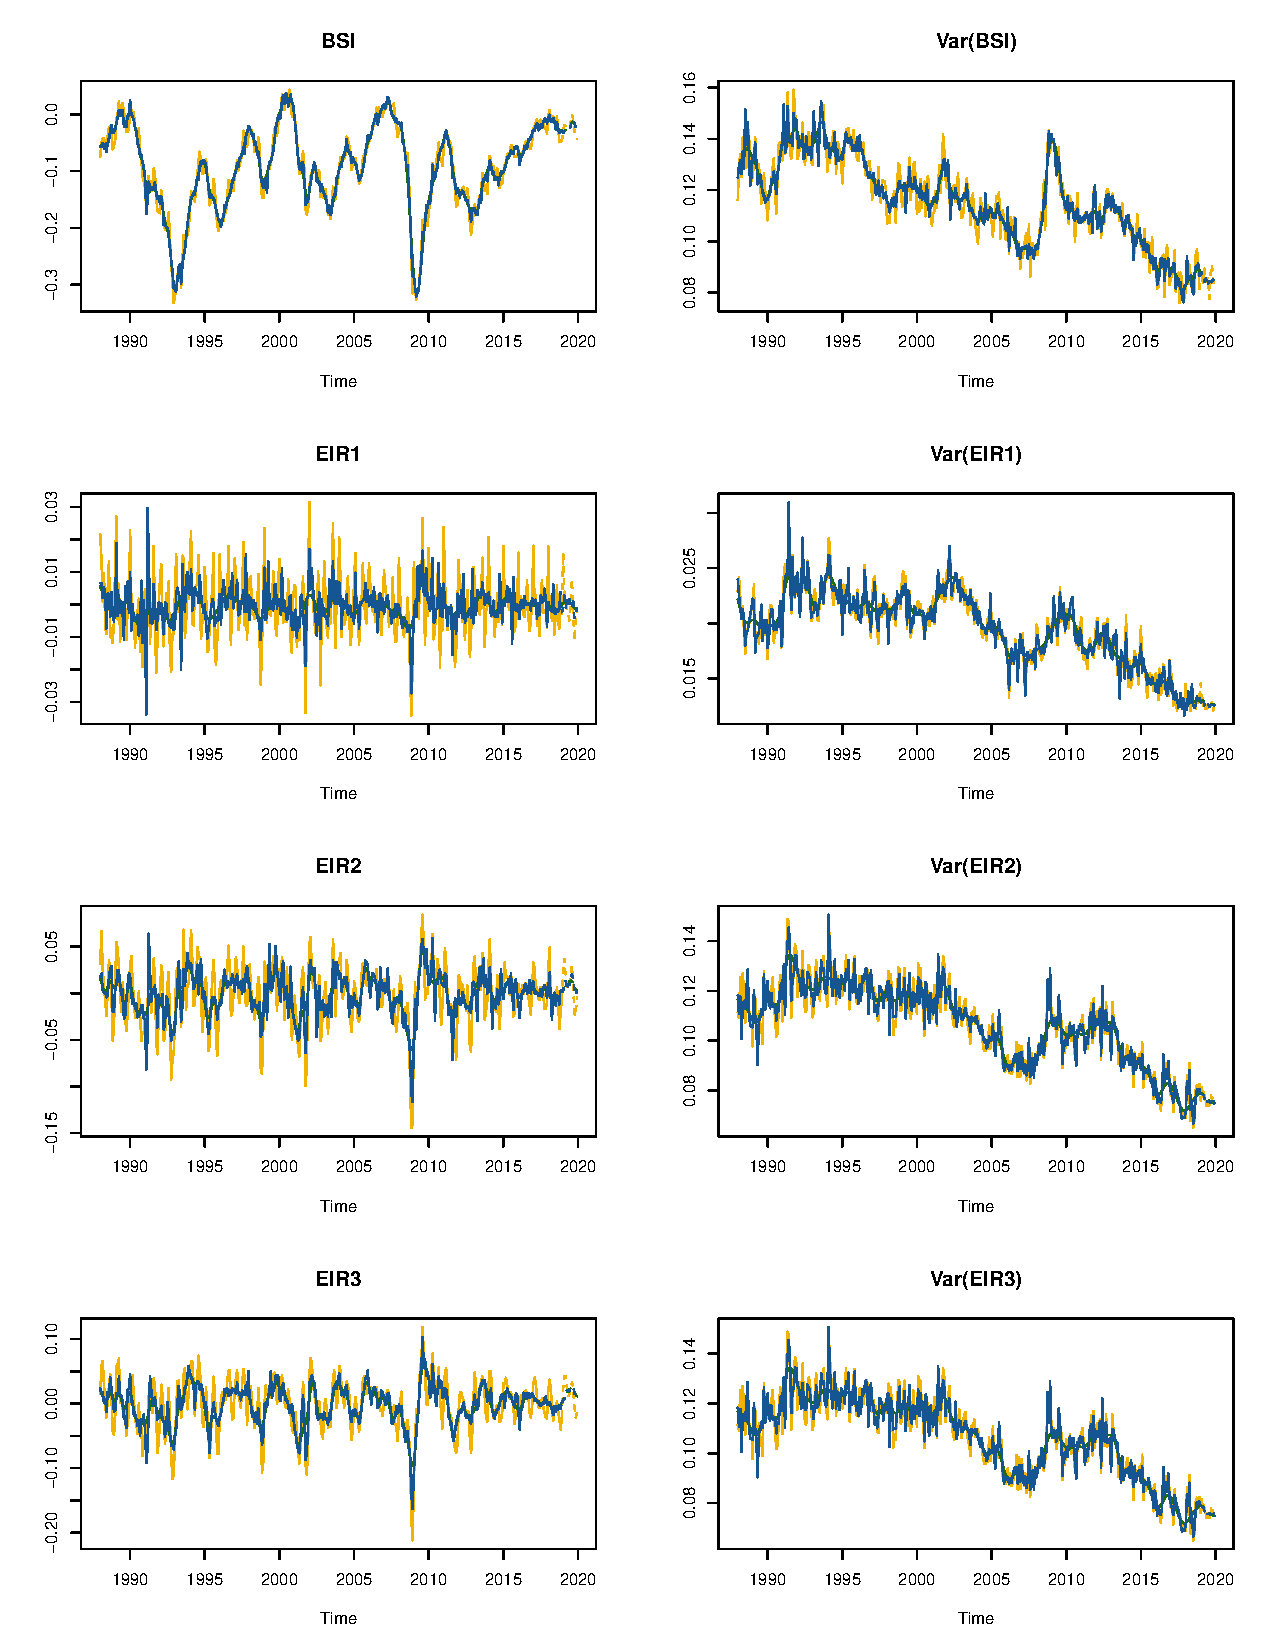
\includegraphics[scale=0.75]{Graphs/RJDemetra_plots.pdf}
    \caption{Plot of the industry business survey indicator (NS975), the indicator of the evolution of individual responses with the previous month (EIR1), two months (EIR2) and three months  earlier (EIR3), with for each of them, their variance. The yellow lines are the raw data, the blue lines the seasonally corrected data and the green line is the trend of the variable.}
    \label{fig:seasonal ajusted rjdemetra}
\end{figure}


\begin{figure}
\begin{subfigure}{.5\textwidth}
  \centering
  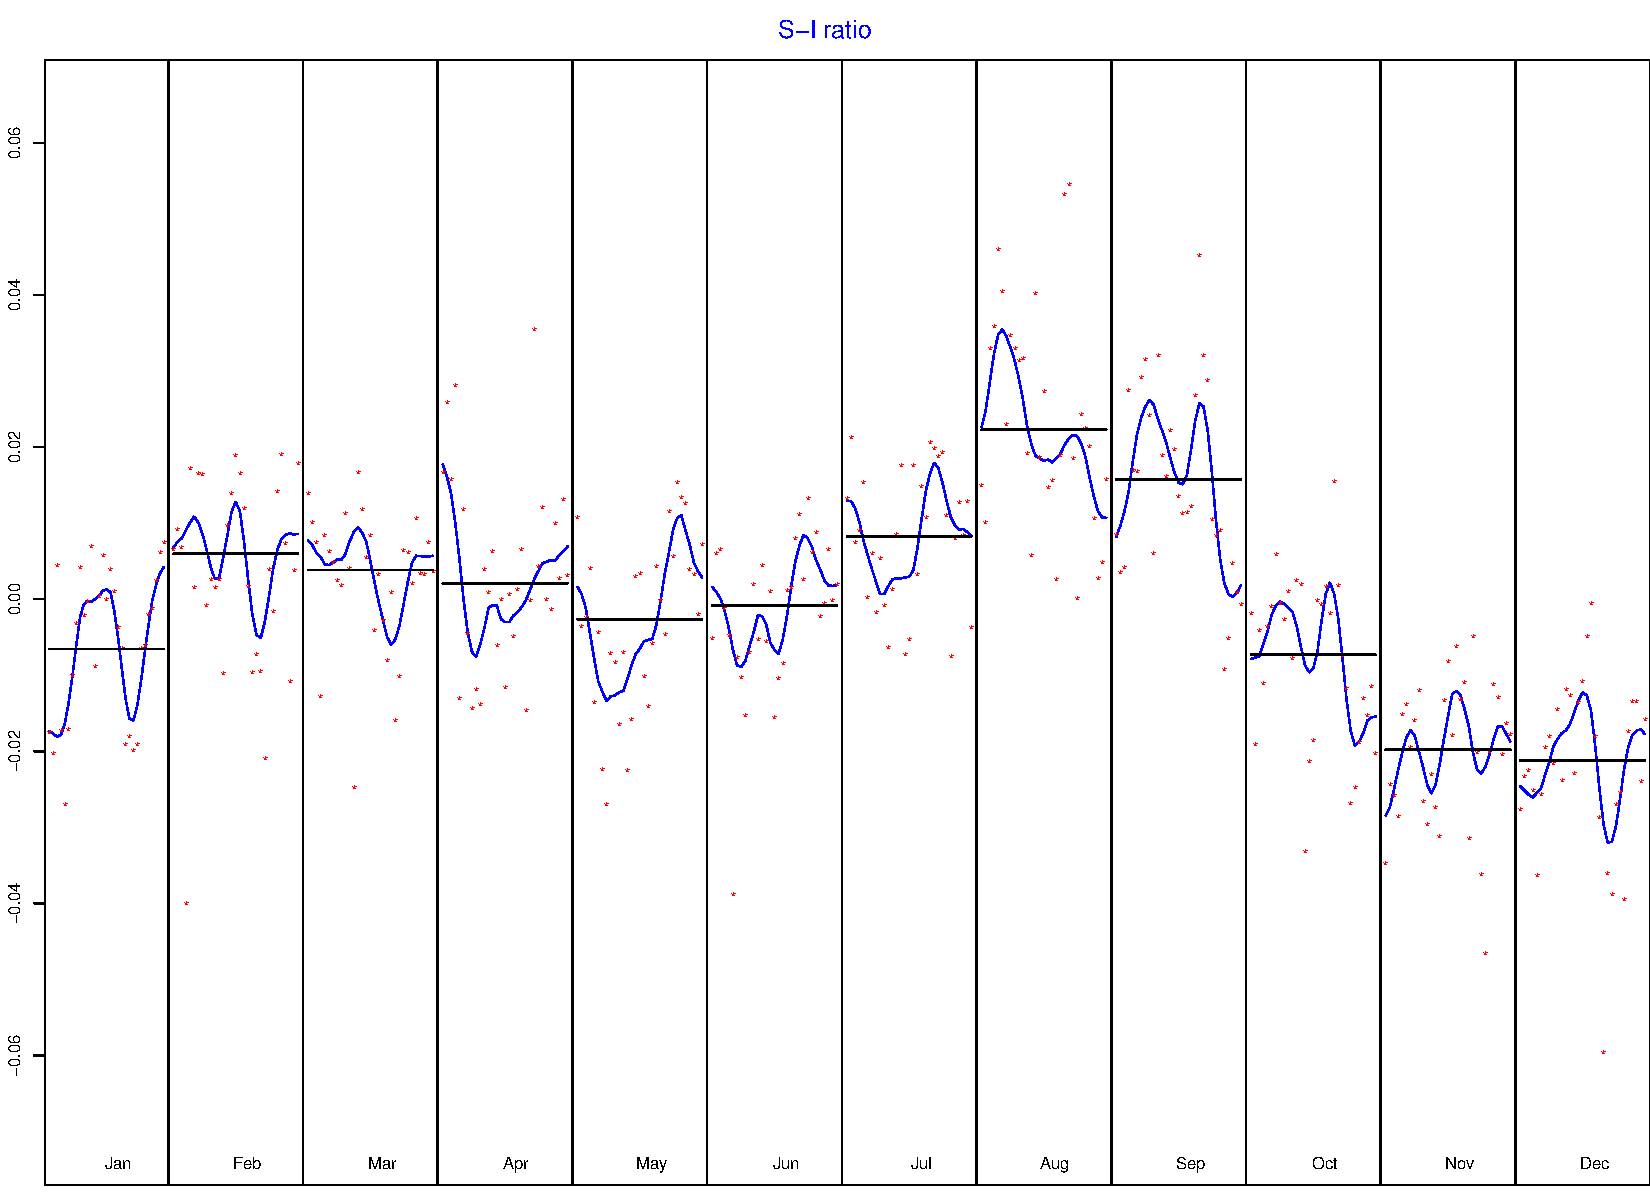
\includegraphics[width=.8\linewidth]{Graphs/S-I_1.pdf}
  \caption{BSI}
\end{subfigure}%
\begin{subfigure}{.5\textwidth}
  \centering
  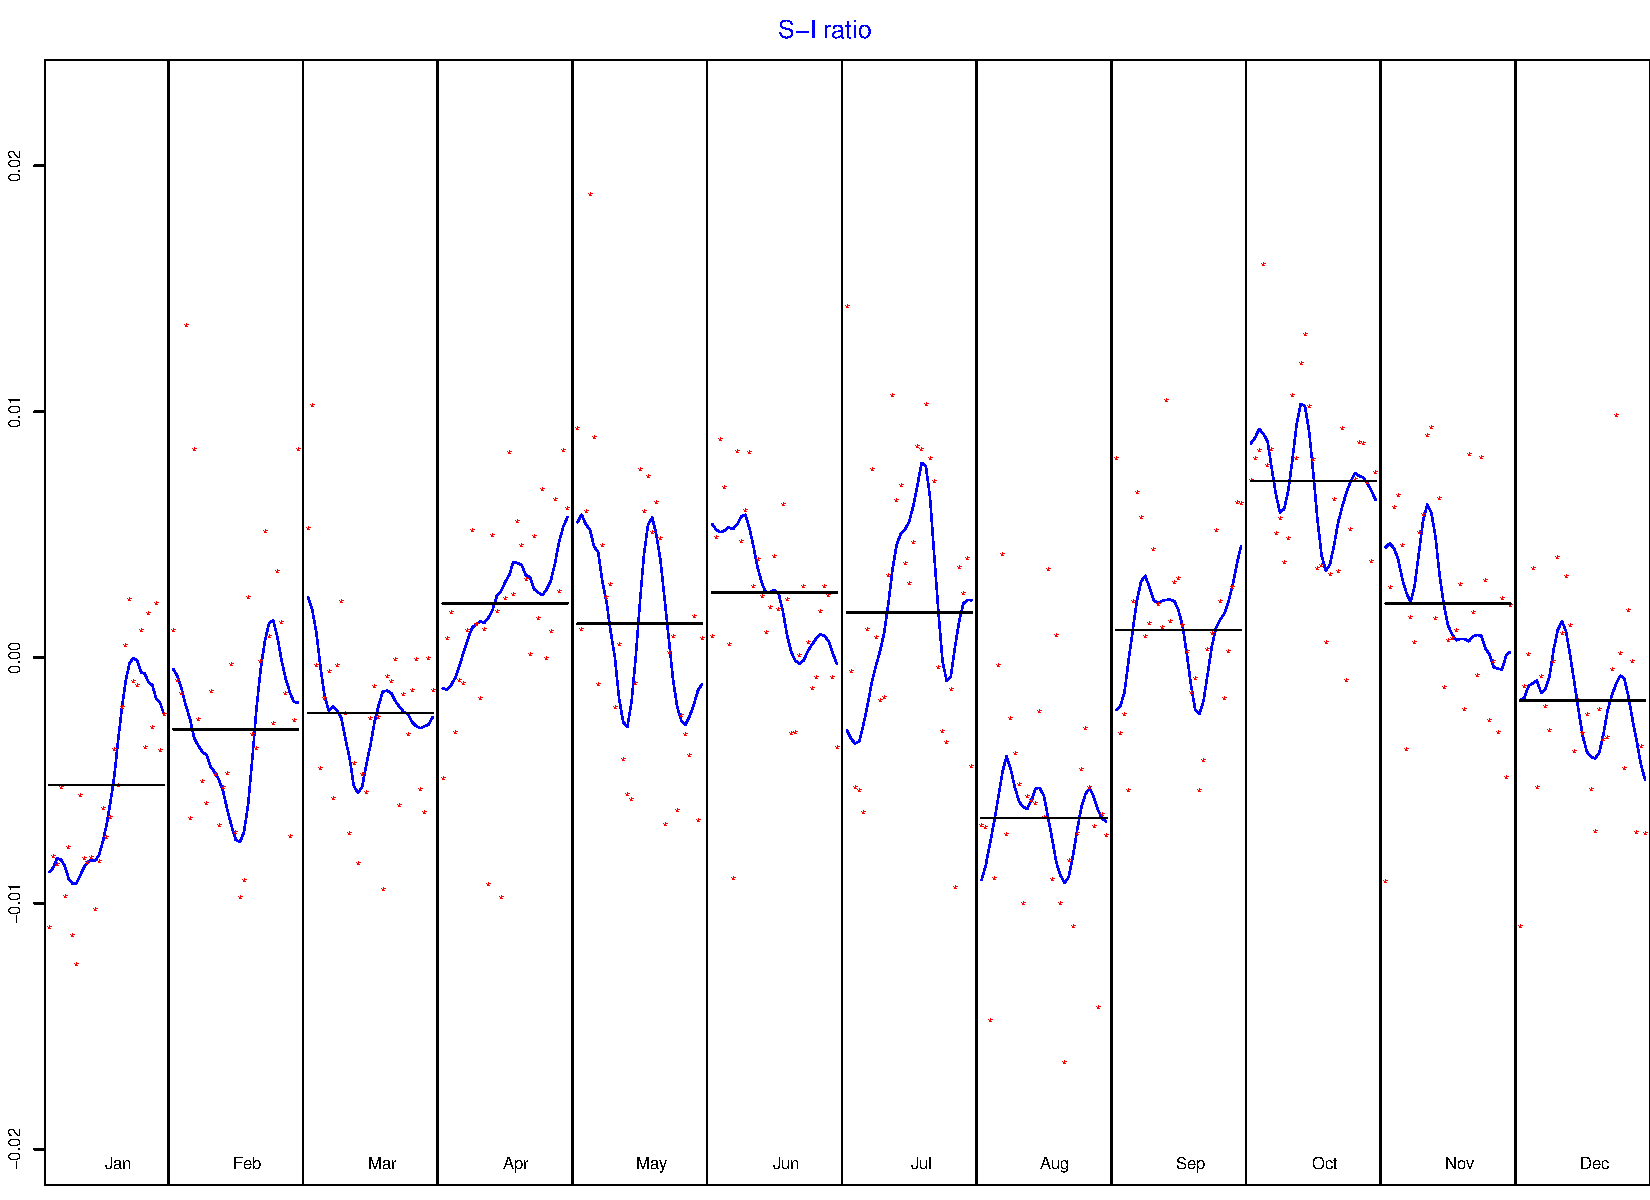
\includegraphics[width=.8\linewidth]{Graphs/S-I_2.pdf}
  \caption{Var(BSI)}
\end{subfigure}
\begin{subfigure}{.5\textwidth}
  \centering
  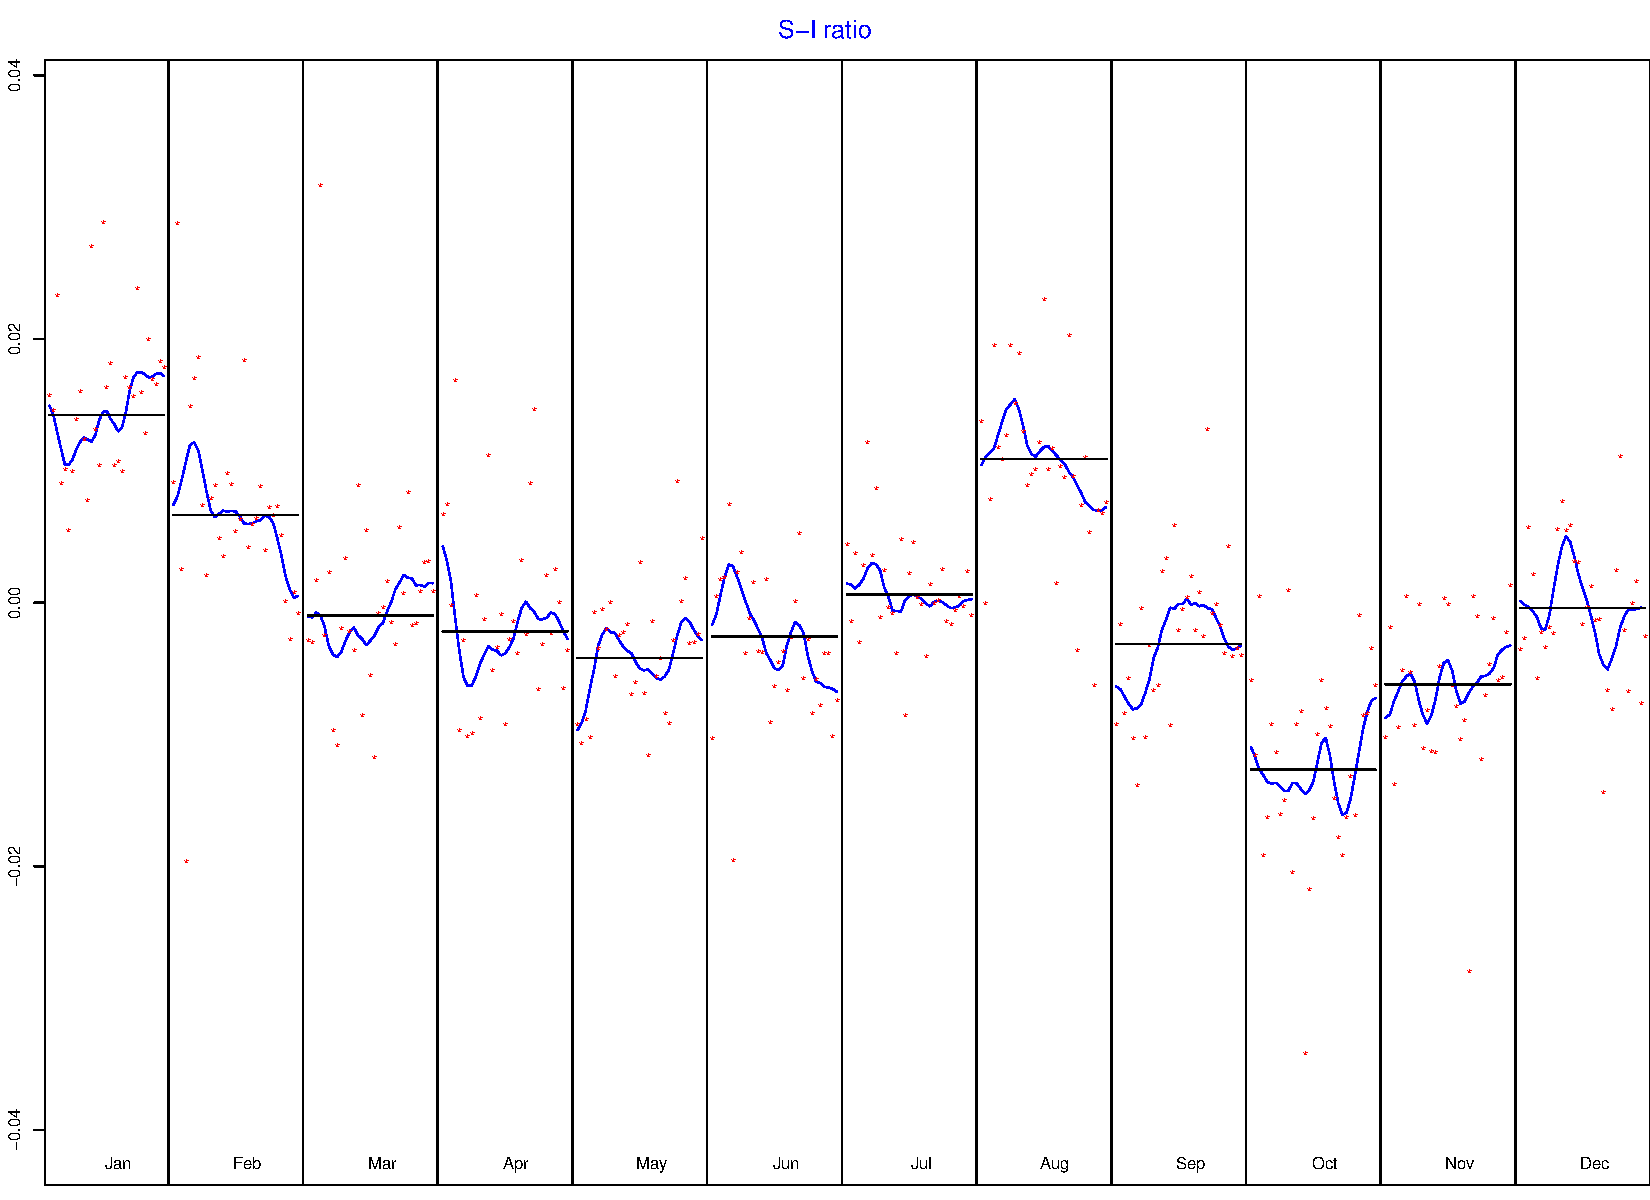
\includegraphics[width=.8\linewidth]{Graphs/S-I_3.pdf}
  \caption{EIR1}
\end{subfigure}
\begin{subfigure}{.5\textwidth}
  \centering
  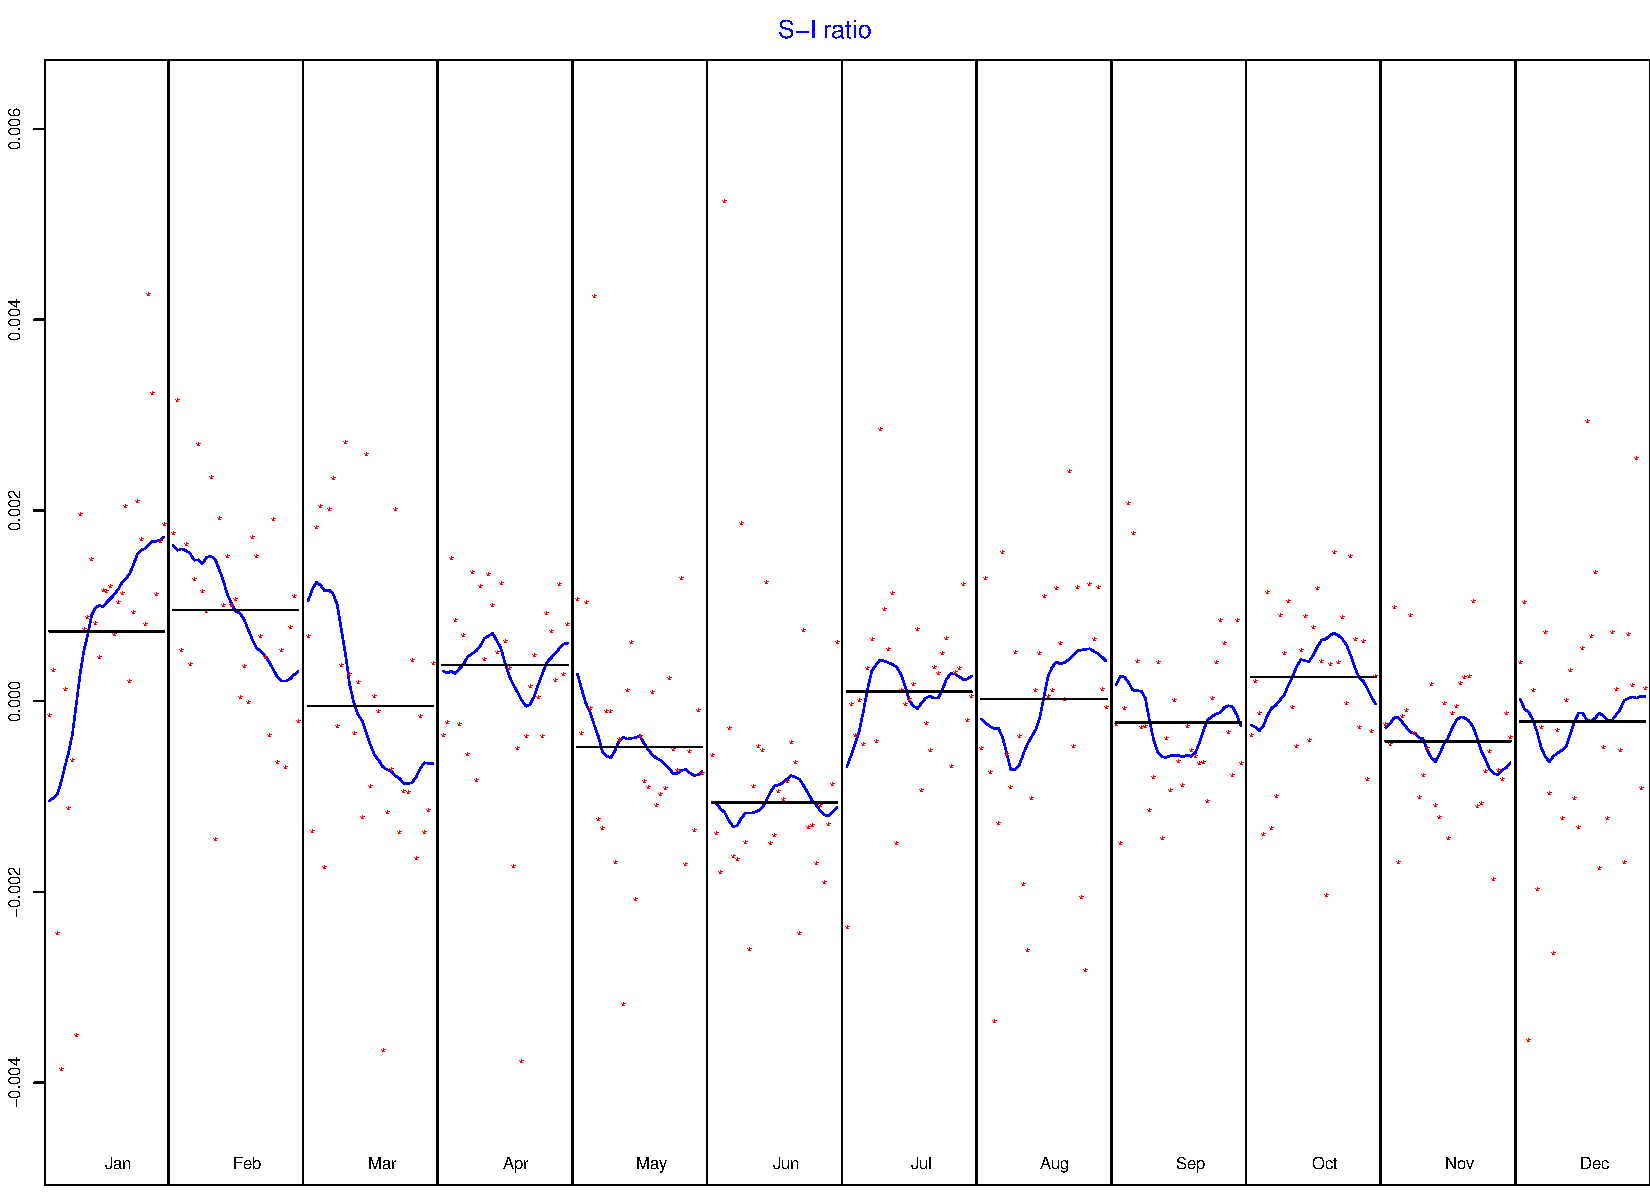
\includegraphics[width=.8\linewidth]{Graphs/S-I_4.pdf}
  \caption{Var(EIR1)}
\end{subfigure}
\begin{subfigure}{.5\textwidth}
  \centering
  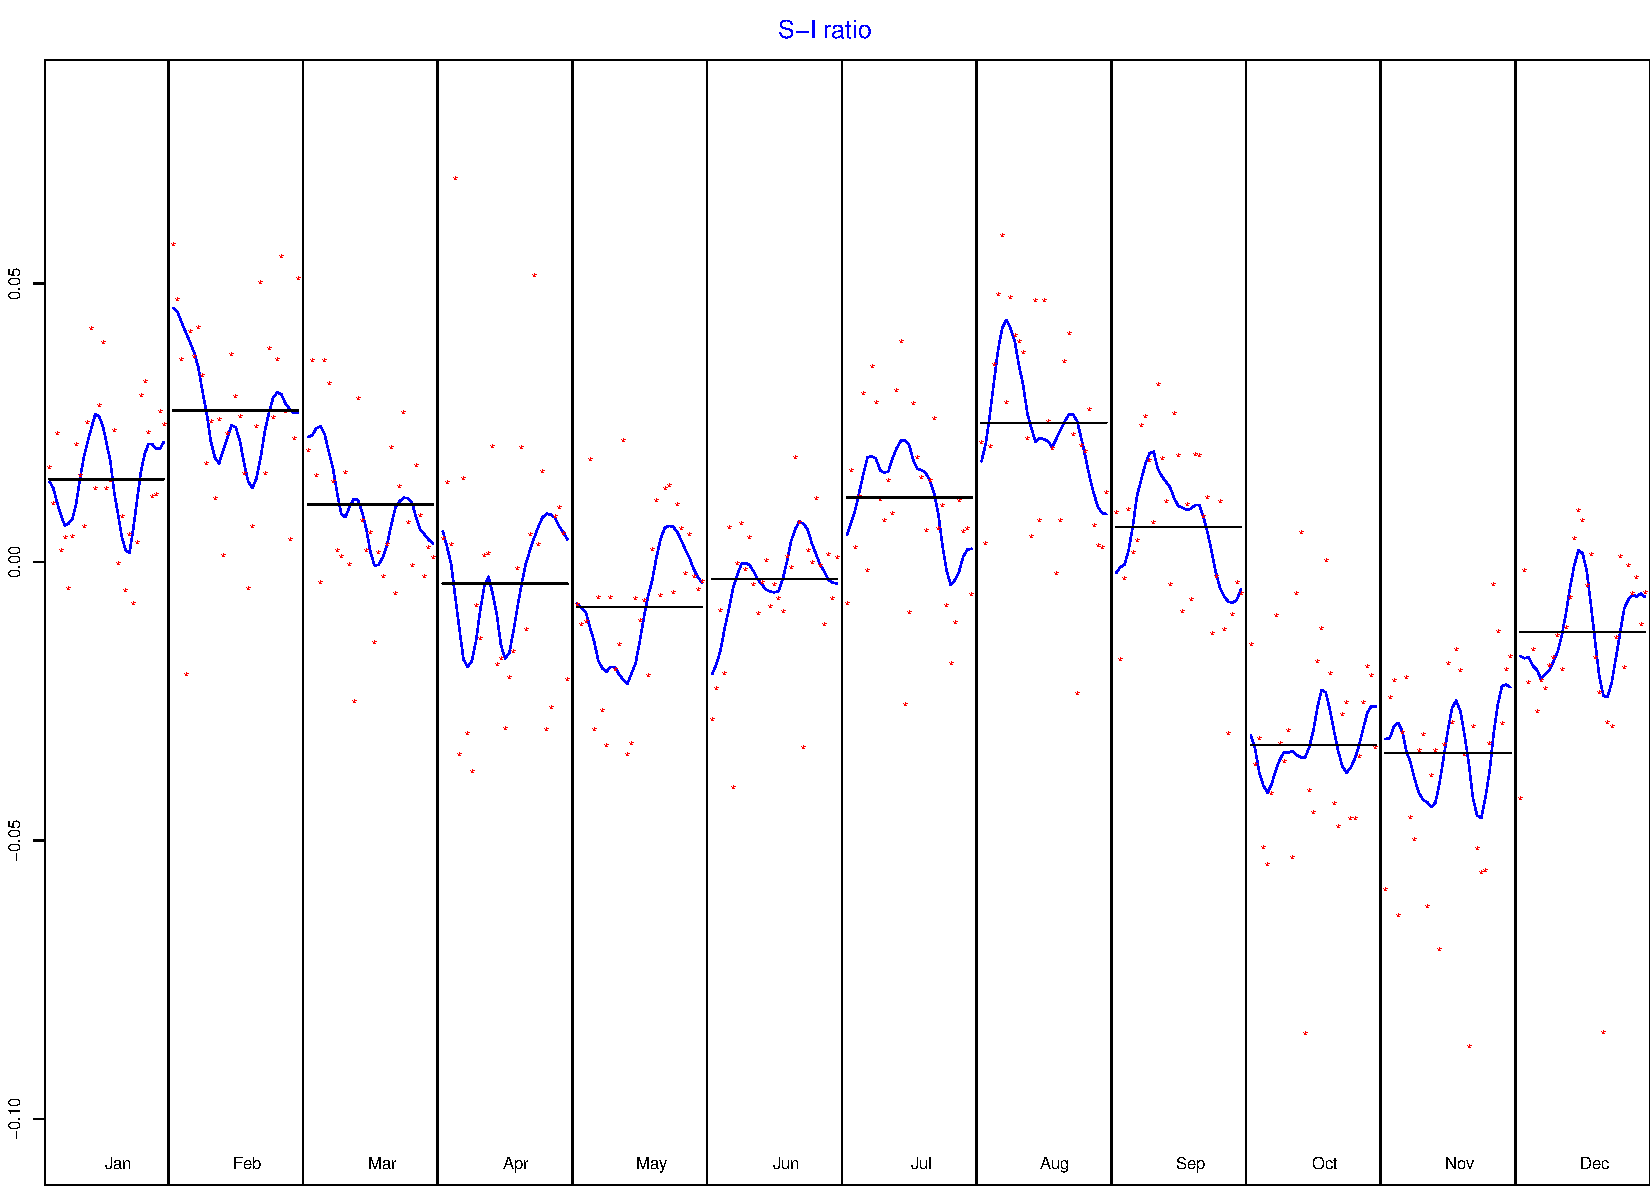
\includegraphics[width=.8\linewidth]{Graphs/S-I_5.pdf}
  \caption{EIR2}
\end{subfigure}
\begin{subfigure}{.5\textwidth}
  \centering
  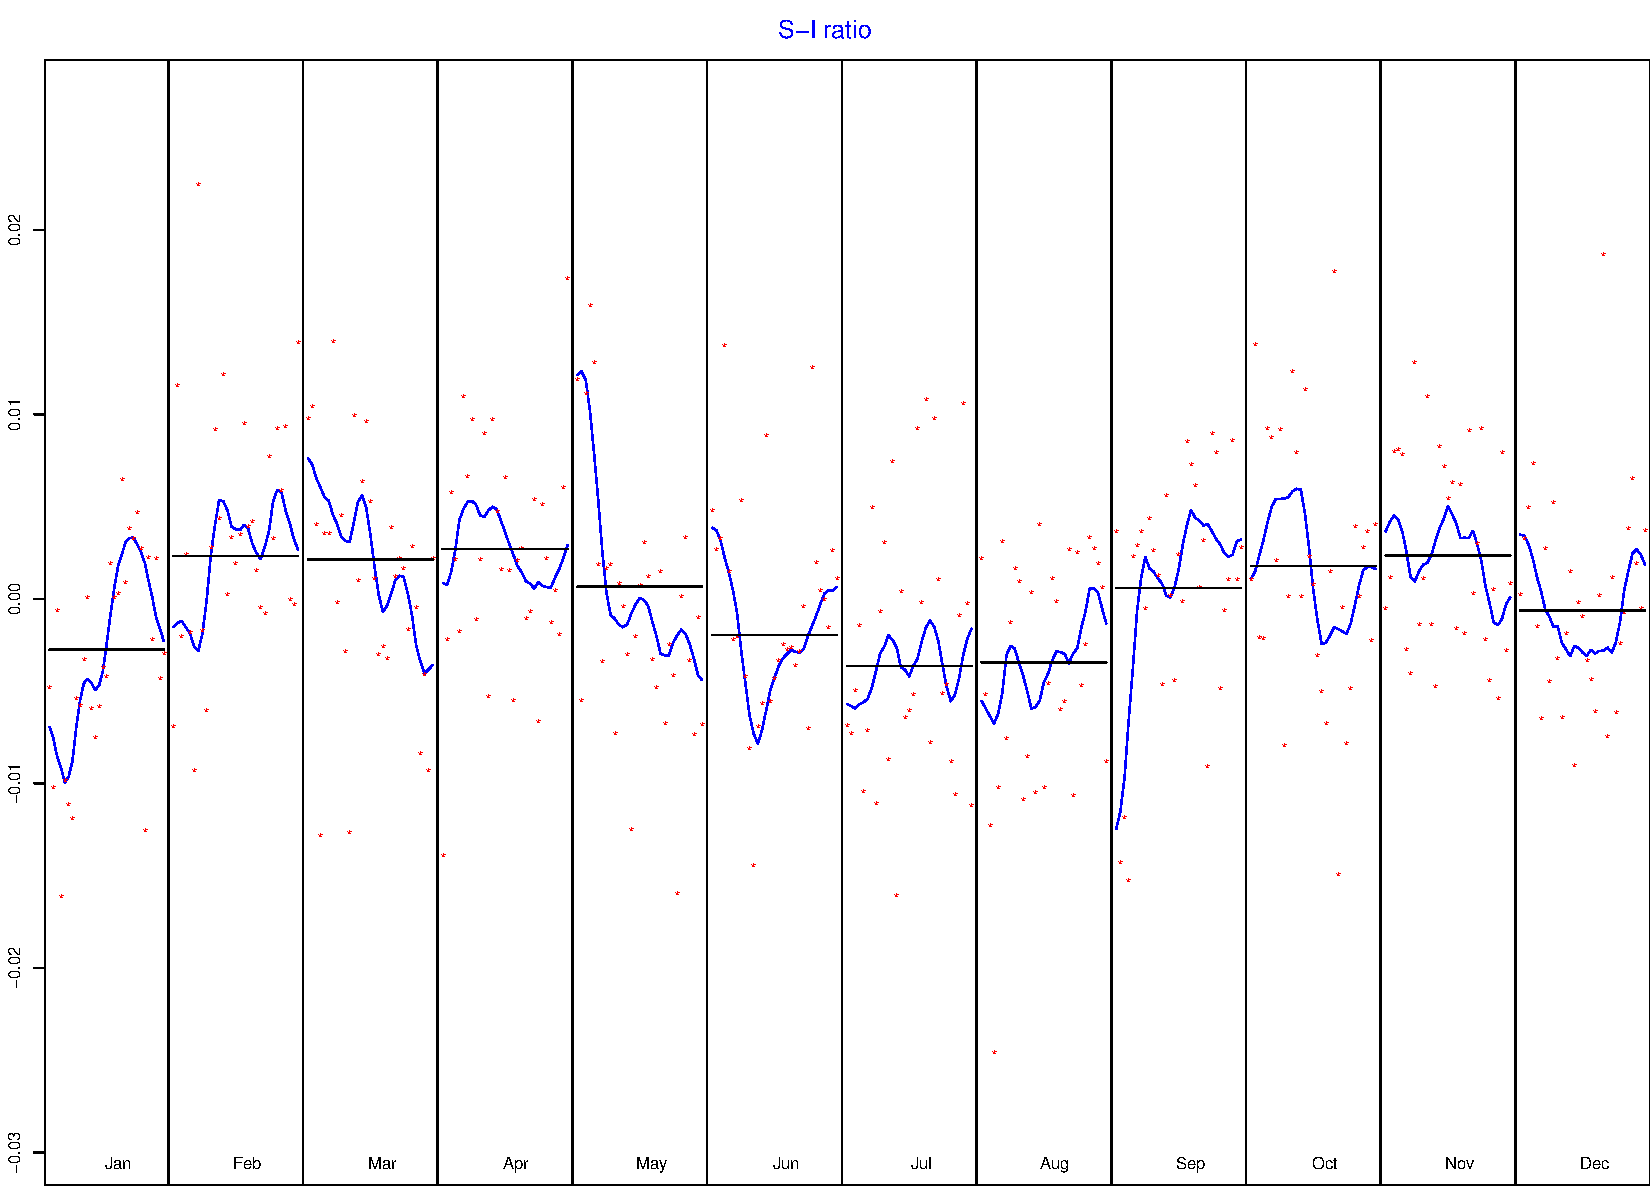
\includegraphics[width=.8\linewidth]{Graphs/S-I_6.pdf}
  \caption{Var(EIR2)}
\end{subfigure}
\begin{subfigure}{.5\textwidth}
  \centering
  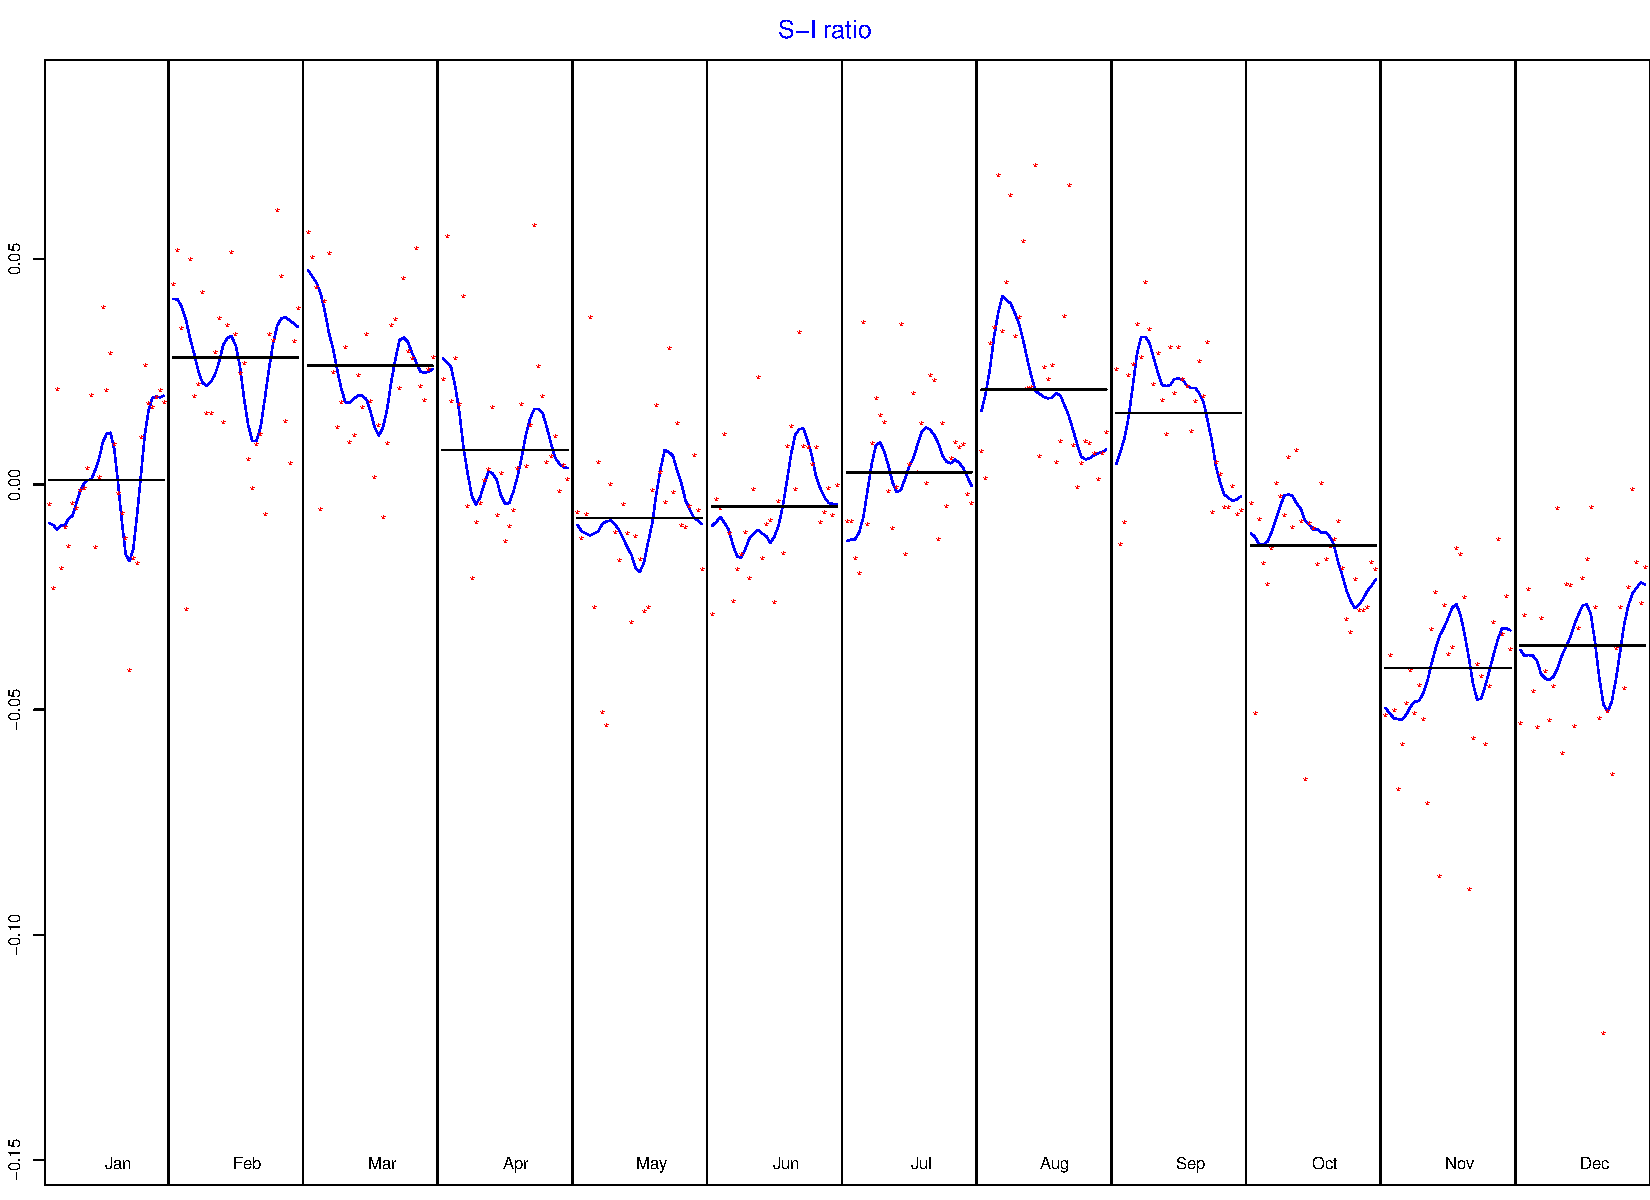
\includegraphics[width=.8\linewidth]{Graphs/S-I_7.pdf}
  \caption{EIR3}
\end{subfigure}
\begin{subfigure}{.5\textwidth}
  \centering
  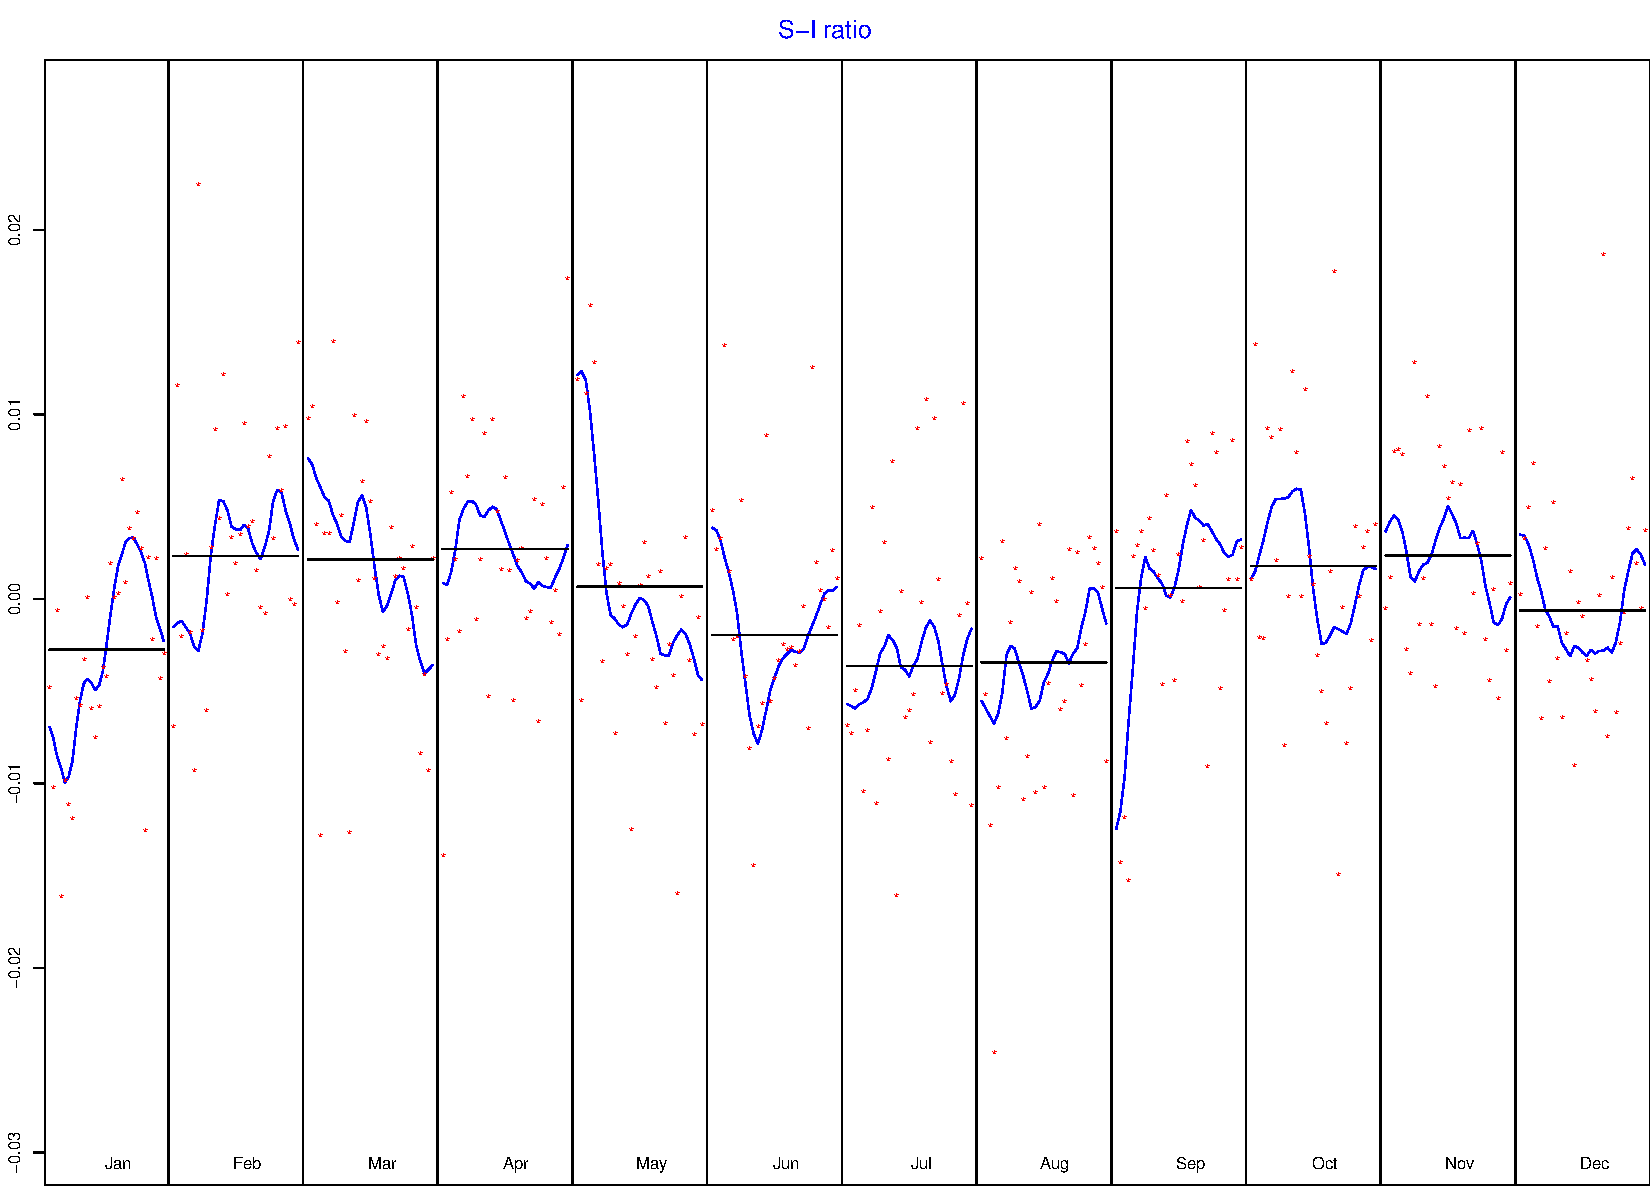
\includegraphics[width=.8\linewidth]{Graphs/S-I_8.pdf}
  \caption{Var(EIR3)}
\end{subfigure}
\caption{plots of....}
\label{fig:S-I seasonal correction RJDemetra}
\end{figure}





\chapter{Exploratory Analysis}

The previous chapter already did some of the exploratory analysis.

We will here have some further observations based on the time trends of the different variables at hand.
In a second time w


\subsubsection{Data At hand}

Small remember
- Four questions summarized together from the industry survey
- 1988 - 2018
- BSI, var BSI, EIR and EIR2

Some things have to be looked at before starting the modelling process

NON Weighted ! to complicated

\section{The industry business survey indicator, the individual evolution in responses and their variances}

 \textbf{plot of the different variables}


\section{Correlations Analysis}

There are three different correlations that need to be looked at

\subsection{Correlation between questions}

\begin{table}[H] \centering 
  \caption{Correlation Matrix} 
  \label{tab:corr questions} 
\begin{tabular}{@{\extracolsep{5pt}} ccccc} 
\\[-1.8ex]\hline 
\hline \\[-1.8ex] 
 & E\_1 & E\_2 & E\_3 & E\_4 \\ 
\hline \\[-1.8ex] 
E\_1 & $1$ & $0.262$ & $0.412$ & $0.416$ \\ 
E\_2 & $0.262$ & $1$ & $0.939$ & $0.876$ \\ 
E\_3 & $0.412$ & $0.939$ & $1$ & $0.938$ \\ 
E\_4 & $0.416$ & $0.876$ & $0.938$ & $1$ \\ 
\hline \\[-1.8ex] 
\end{tabular} 
\end{table}
 
\begin{table}[H] \centering 
  \caption{Correlation Matrix} 
  \label{tab:corr questions} 
\begin{tabular}{@{\extracolsep{5pt}} ccccc} 
\\[-1.8ex]\hline 
\hline \\[-1.8ex] 
 & E\_1 & E\_2 & E\_3 & E\_4 \\ 
\hline \\[-1.8ex] 
E\_1 & $1$ & $0.262$ & $0.412$ & $0.416$ \\ 
E\_2 &  & $1$ & $0.939$ & $0.876$ \\ 
E\_3 &  &  & $1$ & $0.938$ \\ 
E\_4 &  &  &  & $1$ \\ 
\hline \\[-1.8ex] 
\end{tabular} 
\end{table}

\subsection{Correlation with GDP}

Belgian industry claims 25\% of the labour force in Belgium and have been shown as been the best indicator to predict the year to year GDP
cite{Alain Quartier and Isabelle}


\subsubsection*{GDP vs GDP YoY}

\begin{table}[H] \centering 
  \caption{Correlation Matrix} 
  \label{tab:corr gdp} 
\begin{tabular}{@{\extracolsep{5pt}} cccccccc} 
\\[-1.8ex]\hline 
\hline \\[-1.8ex] 
 & GDP & GDP\_year & E\_I & E\_1 & E\_2 & E\_3 & E\_4 \\ 
\hline \\[-1.8ex] 
GDP & $1$ & $0.628$ & $0.502$ & $0.222$ & $0.439$ & $0.473$ & $0.556$ \\ 
GDP\_year & $0.628$ & $1$ & $0.707$ & $0.092$ & $0.729$ & $0.703$ & $0.717$ \\ 
E\_I & $0.502$ & $0.707$ & $1$ & $0.483$ & $0.952$ & $0.982$ & $0.963$ \\ 
E\_1 & $0.222$ & $0.092$ & $0.483$ & $1$ & $0.266$ & $0.414$ & $0.406$ \\ 
E\_2 & $0.439$ & $0.729$ & $0.952$ & $0.266$ & $1$ & $0.942$ & $0.886$ \\ 
E\_3 & $0.473$ & $0.703$ & $0.982$ & $0.414$ & $0.942$ & $1$ & $0.938$ \\ 
E\_4 & $0.556$ & $0.717$ & $0.963$ & $0.406$ & $0.886$ & $0.938$ & $1$ \\ 
%\vdots & \vdots & \vdots & \vdots & \vdots & \vdots & \vdots \\
\hline \\[-1.8ex] 
\end{tabular} 
\end{table} 


\begin{figure}[H]
    \centering
    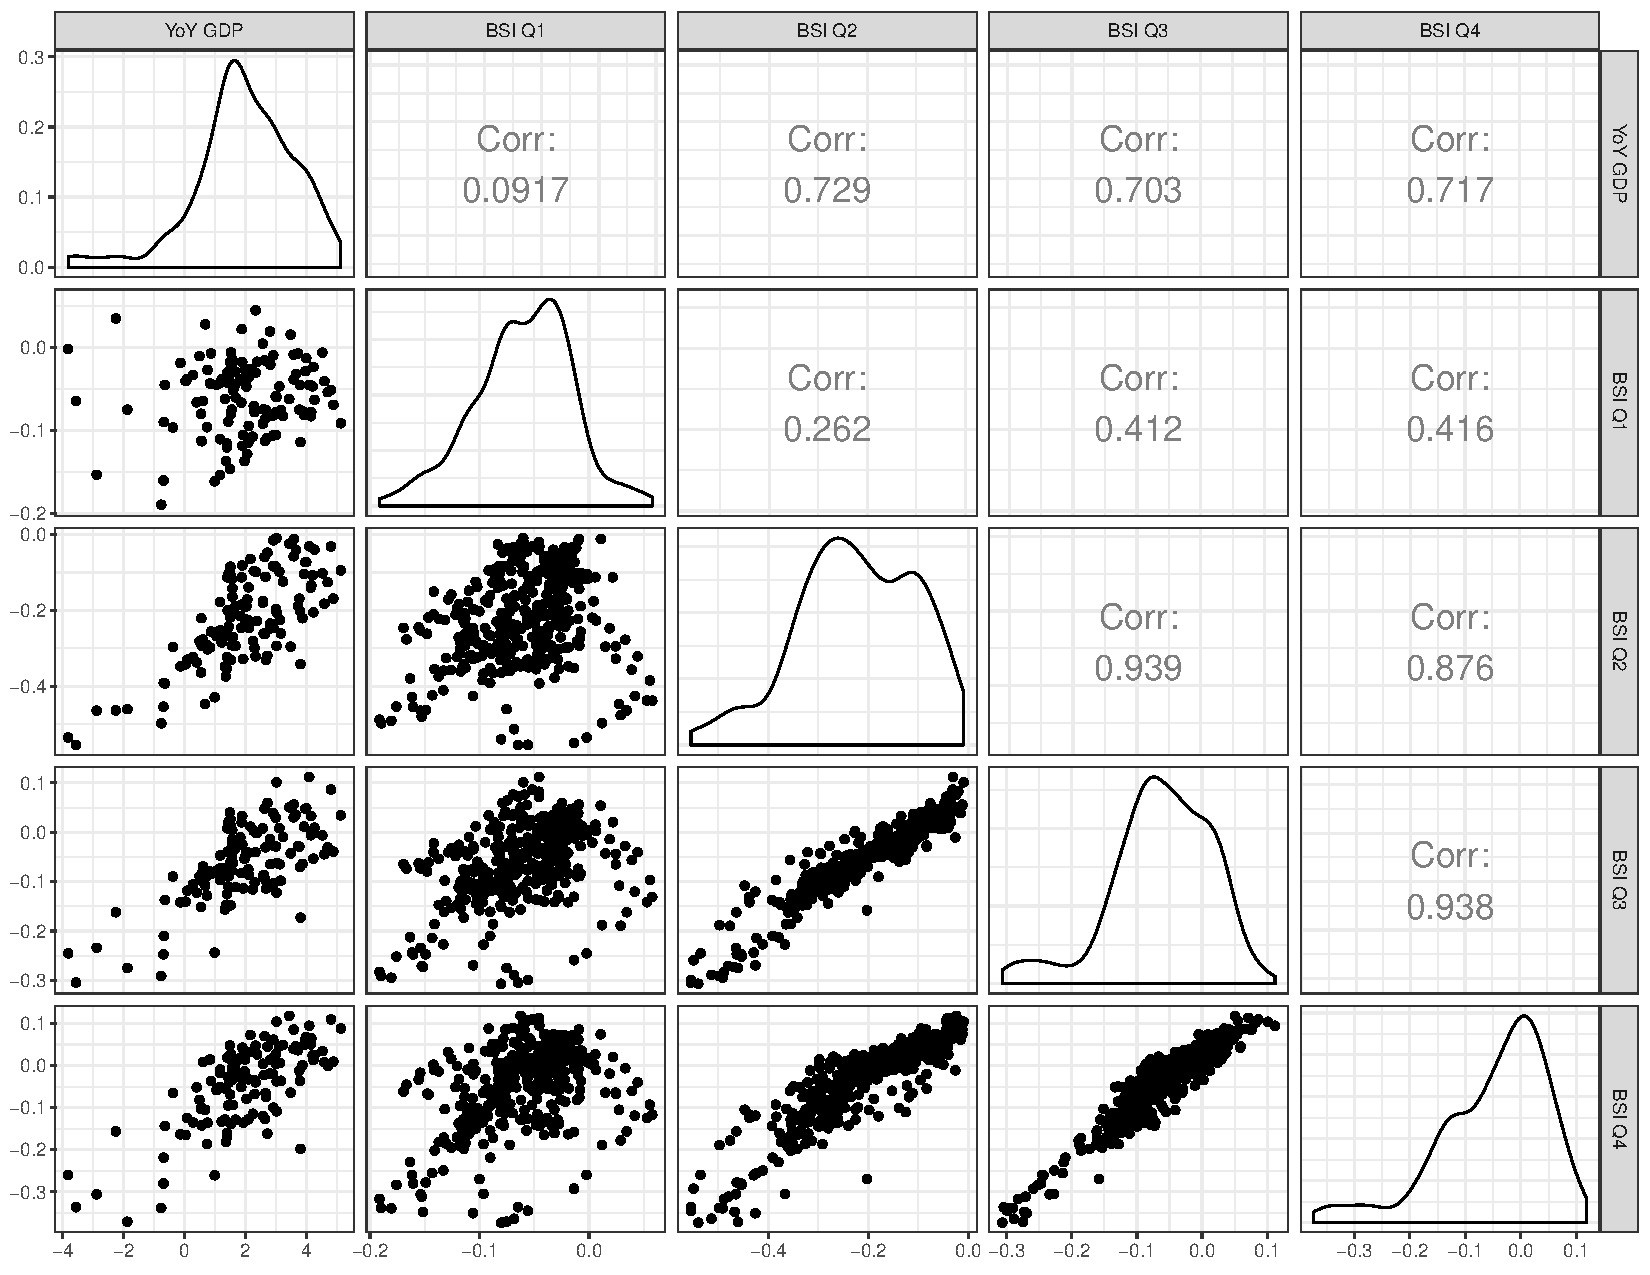
\includegraphics[scale=0.5]{Graphs/Corr_GDP_Questions.pdf}
    \caption{Plot }
    \label{fig:ggpairs}
\end{figure}


\begin{table}[H] \centering 
  \caption{Correlation Matrix} 
  \label{tab:corr variables} 
\begin{tabular}{@{\extracolsep{5pt}} ccccccc} 
\\[-1.8ex]\hline 
\hline \\[-1.8ex] 
 & GDP & GDP\_year & E\_I & Var\_I & Z\_I & Var\_Z\_I \\ 
\hline \\[-1.8ex] 
GDP & $1$ & $0.628$ & $0.502$ & $-0.074$ & $0.151$ & $0.021$ \\ 
GDP\_year & $0.628$ & $1$ & $0.707$ & $-0.101$ & $-0.058$ & $0.011$ \\ 
E\_I & $0.502$ & $0.707$ & $1$ & $-0.615$ & $0.166$ & $-0.484$ \\ 
Var\_I & $-0.074$ & $-0.101$ & $-0.615$ & $1$ & $-0.045$ & $0.887$ \\ 
Z\_I & $0.151$ & $-0.058$ & $0.166$ & $-0.045$ & $1$ & $-0.072$ \\ 
Var\_Z\_I & $0.021$ & $0.011$ & $-0.484$ & $0.887$ & $-0.072$ & $1$ \\ 
\hline \\[-1.8ex] 
\end{tabular} 
\end{table} 

\begin{figure}[H]
    \centering
    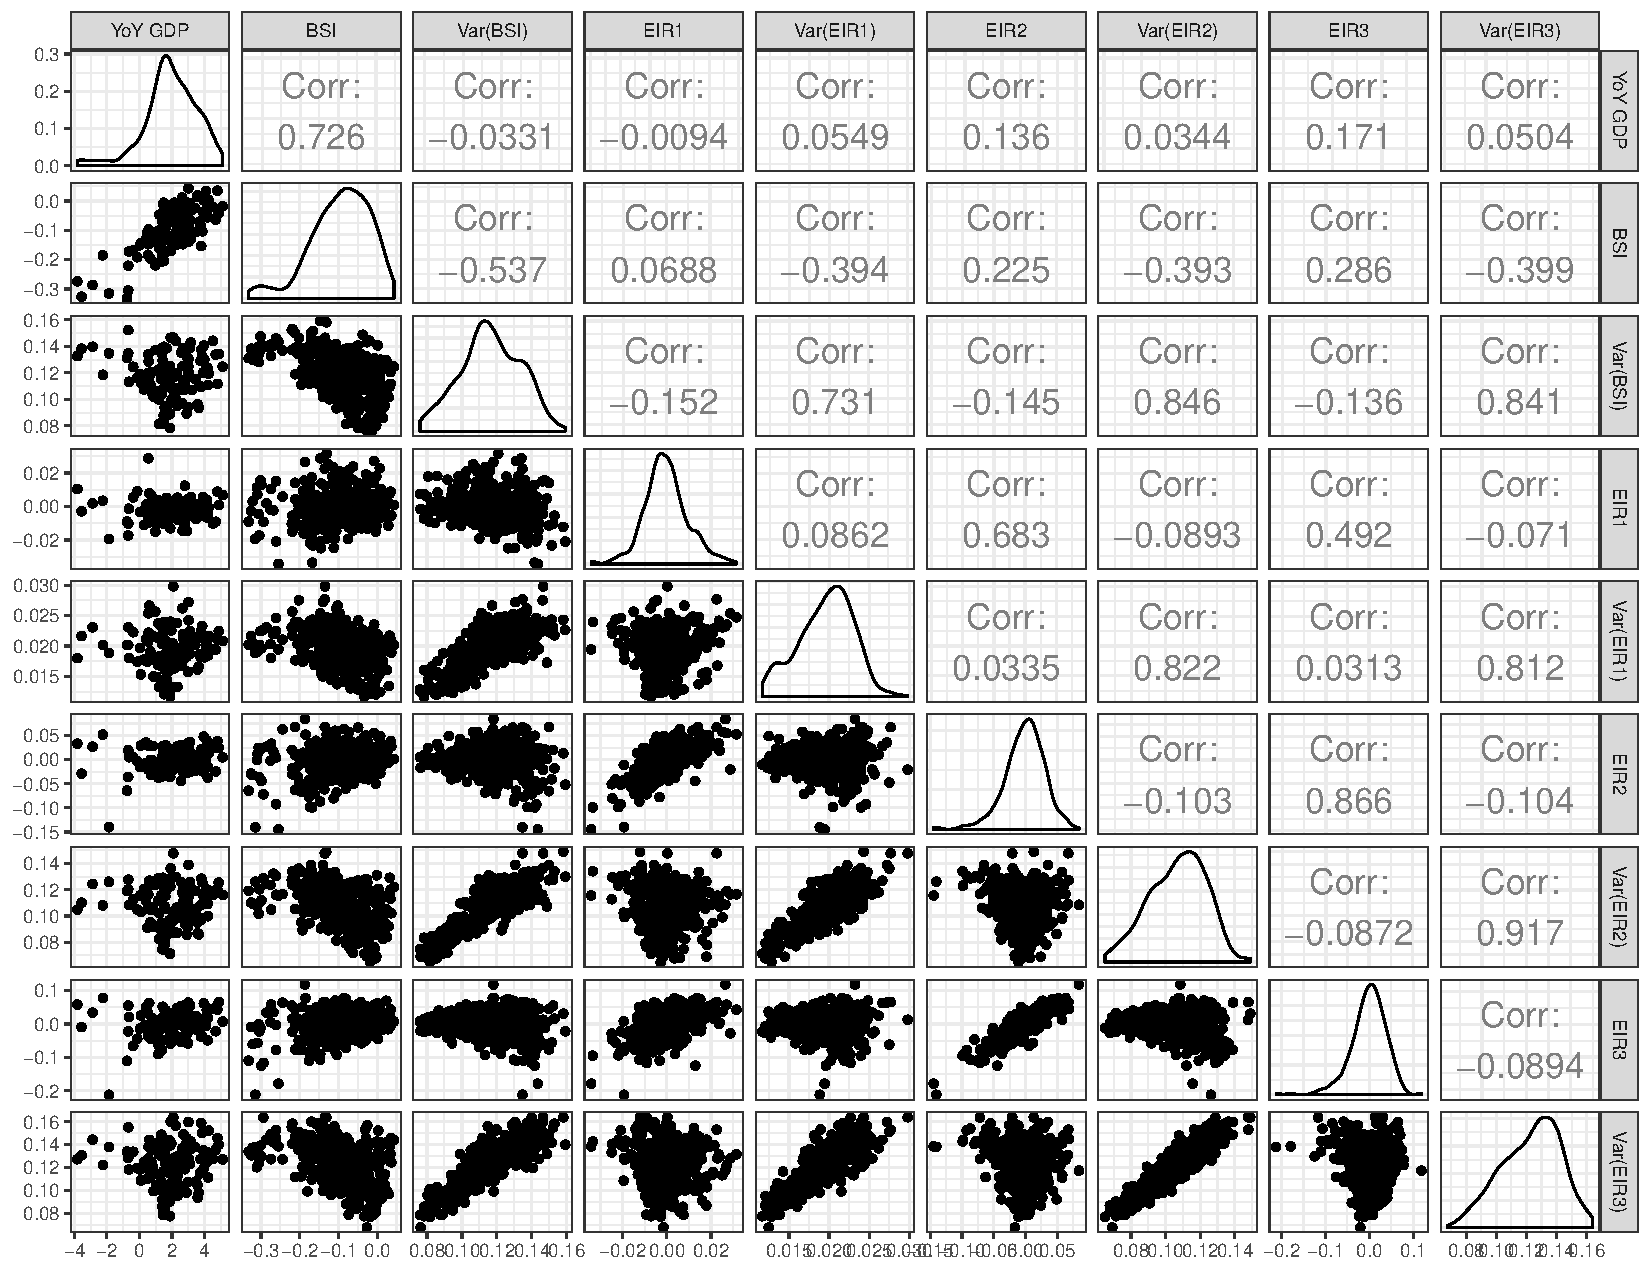
\includegraphics[scale=0.5]{Graphs/corr_indicators.pdf}
    \caption{Plot }
    \label{fig:corr indicators}
\end{figure}

\subsubsection{GDP vs Indicator}

\subsubsection{GDP vs Var}

\subsubsection{GDP vs Z}

\subsubsection{GDP vs Var Z}




\section{Auto-Correlation}

Test stationarity of the time series (ADF)
In order to test the stationarity of the time series, let’s run the Augmented Dickey-Fuller Test using the adf.test() function from the tseries R package.

First set the hypothesis test:

The null hypothesis H0 : that the time series is non stationary The alternative hypothesis HA : that the time series is stationary

adf.test(candyts)

\begin{figure}[H]
    \centering
    \captionsetup{justification=centering}
    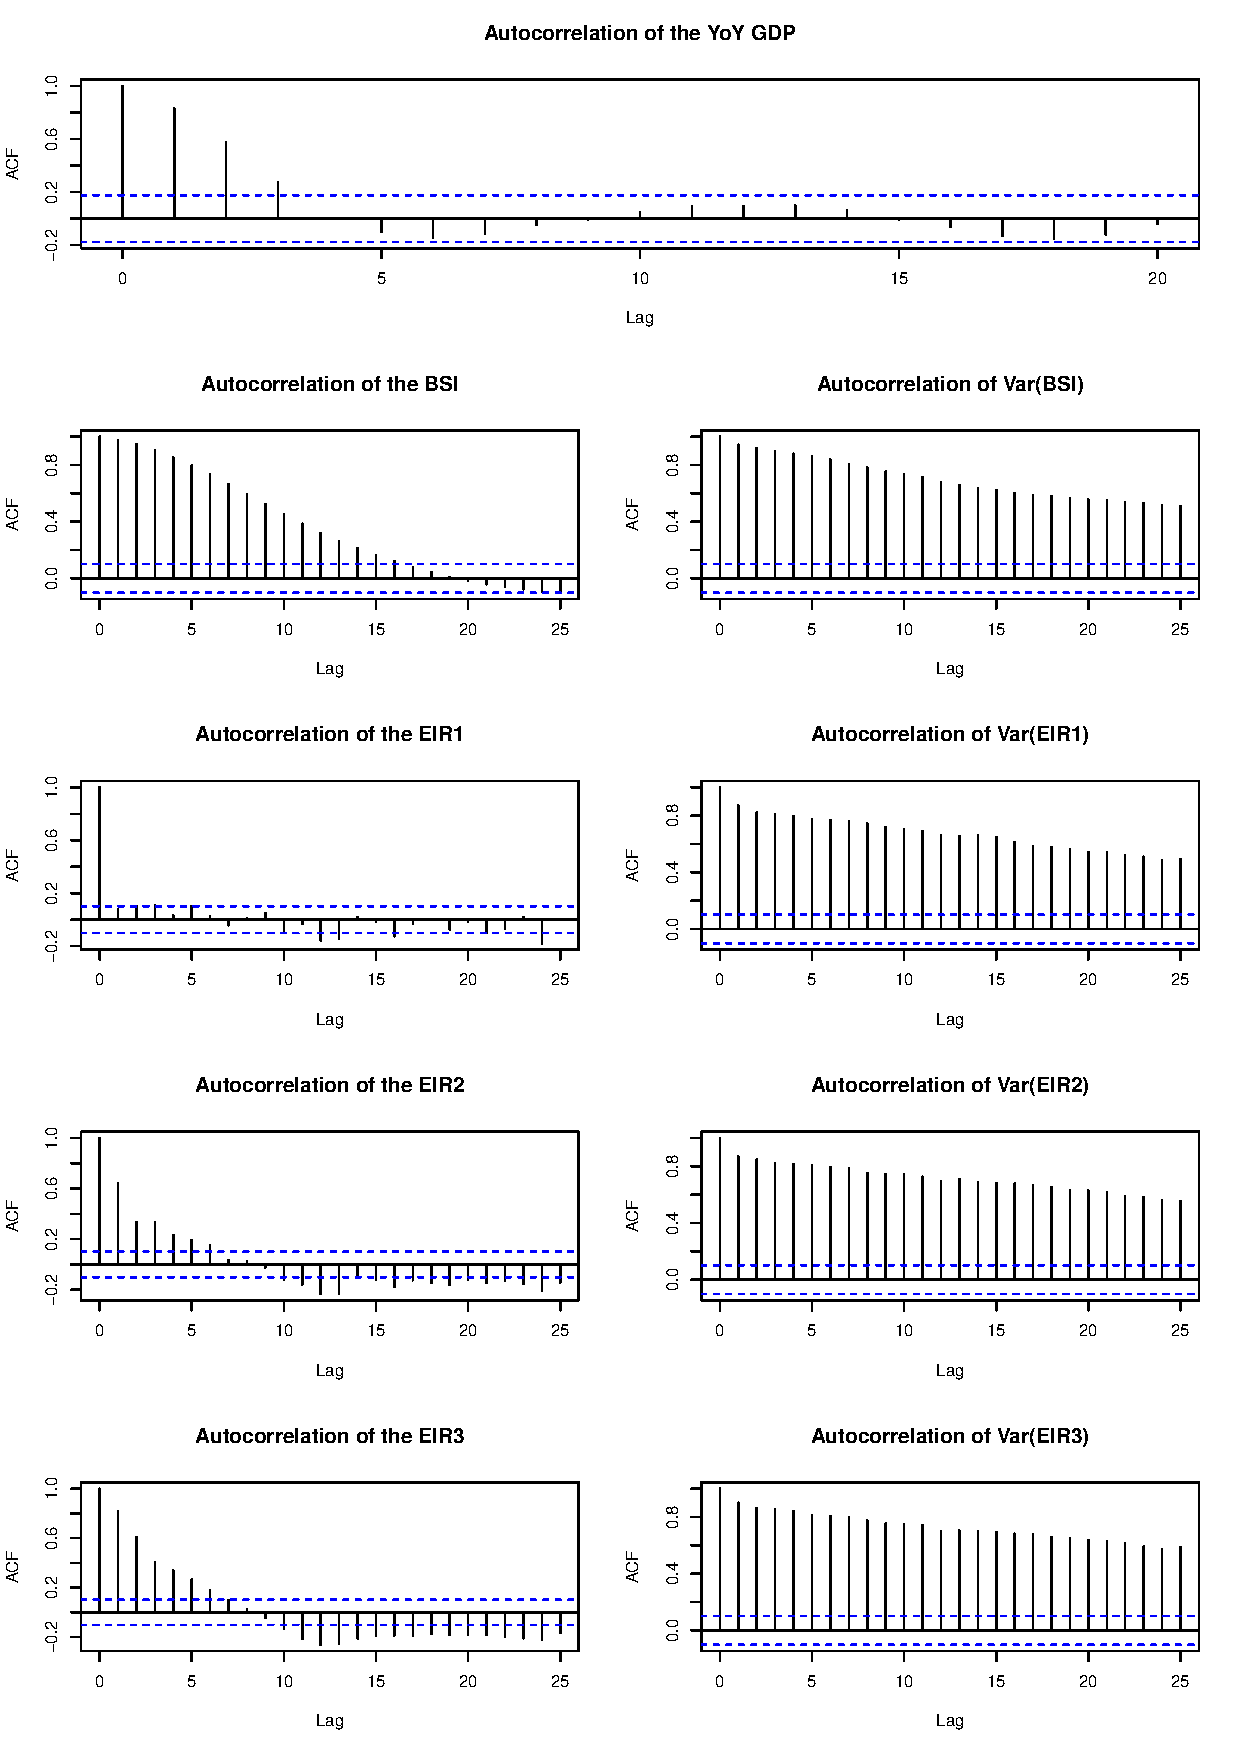
\includegraphics[scale=0.5]{Graphs/ACF.pdf}
    \caption{Plot }
    \label{fig:ACF}
\end{figure}

\begin{figure}[H]
    \centering
    \captionsetup{justification=centering}
    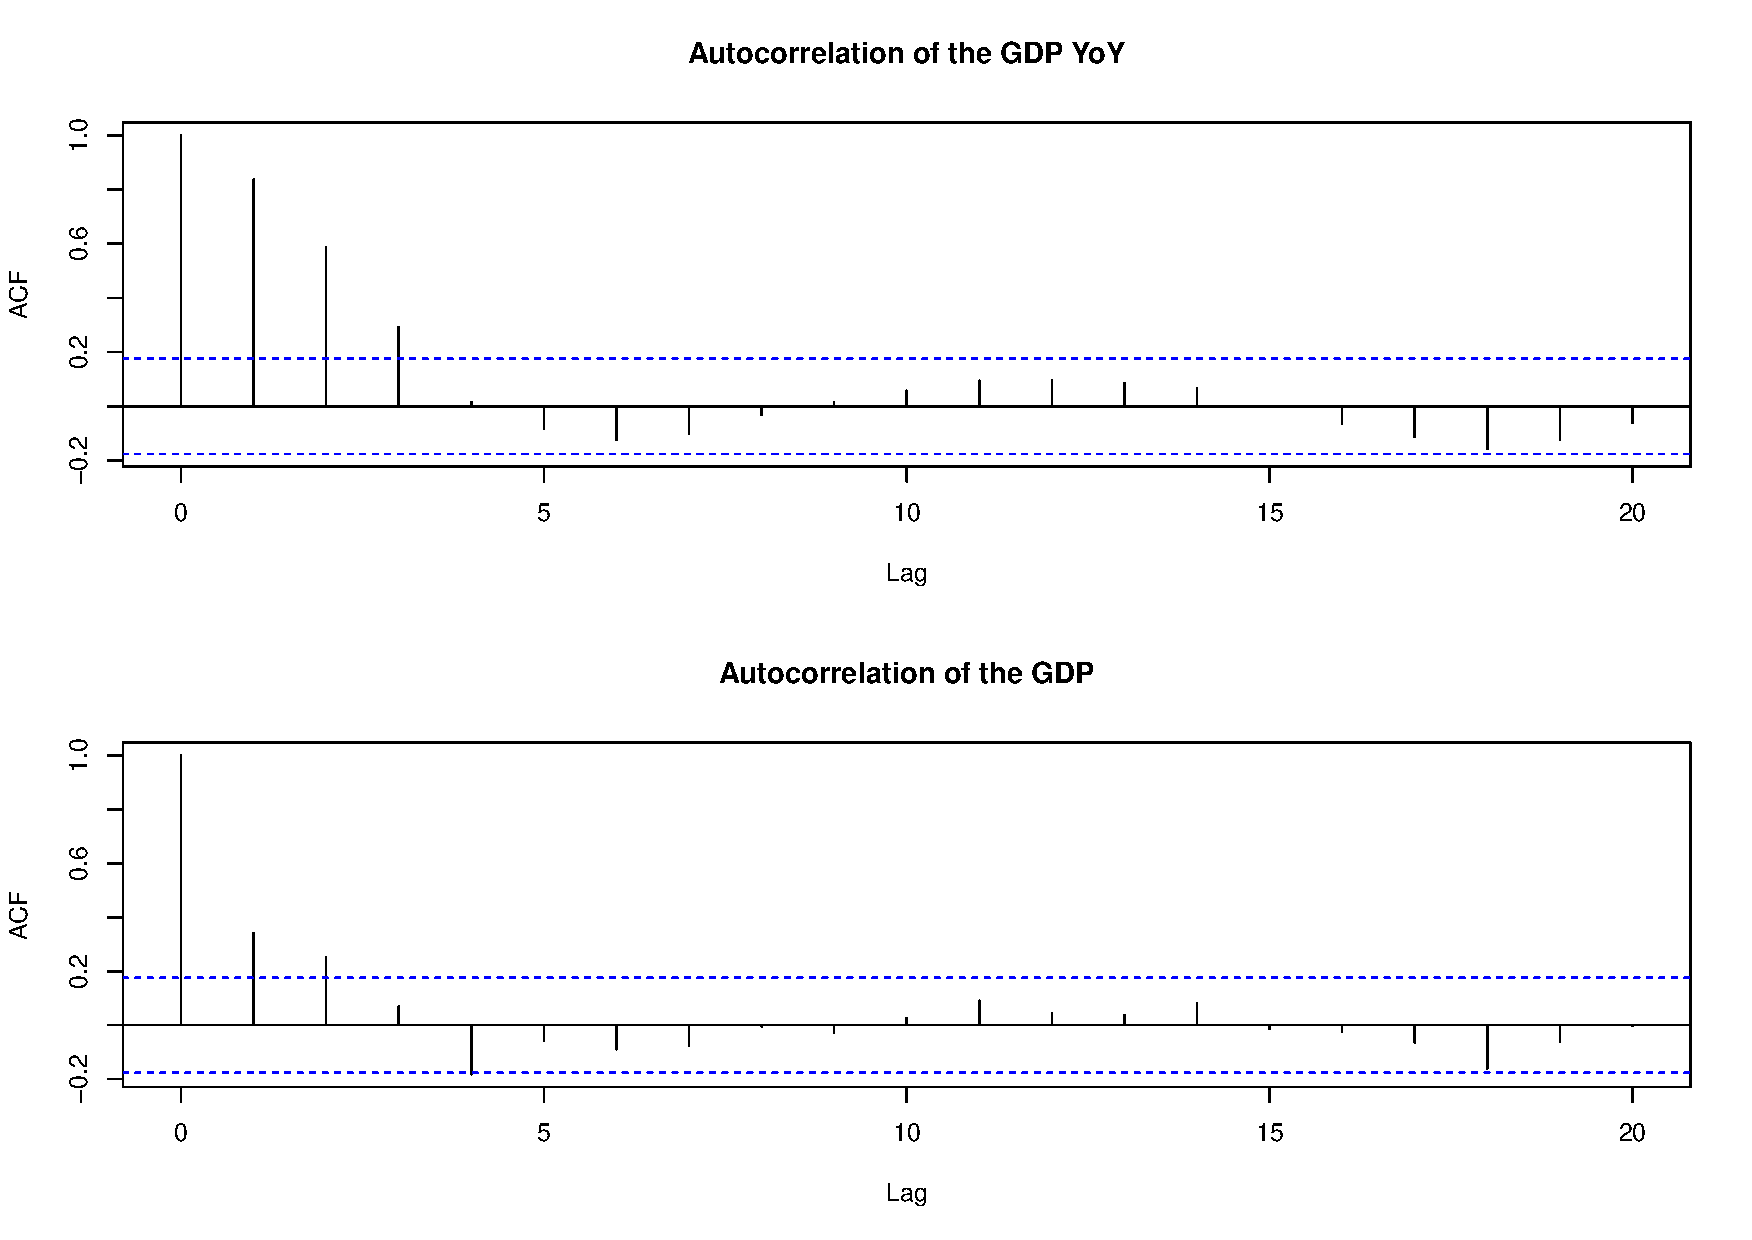
\includegraphics[scale=0.45]{Graphs/ACF_GDP.pdf}
    \caption{Plot }
    \label{fig:ACF_GDP}
\end{figure}


\section{Correlation between Z and Z2 and var(Z) and var(Z2)}


\section{Specificity of question 3 and 4, are peoples predictions correct ?}

\begin{table}[H] \centering 
  \caption{Correlation Matrix} 
  \label{tab:corr question3} 
\begin{tabular}{@{\extracolsep{5pt}} cccccccc} 
\\[-1.8ex]\hline 
\hline \\[-1.8ex] 
 & GDP & GDP\_year & E\_3 & E\_3\_lag1 & E\_3\_lag2 & E\_3\_lag3 & E\_3\_lag4 \\ 
\hline \\[-1.8ex] 
GDP & $1$ & $0.628$ & $0.477$ & $0.520$ & $0.545$ & $0.546$ & $0.531$ \\
GDP\_year & $0.628$ & $1$ & $0.707$ & $0.679$ & $0.673$ & $0.628$ & $0.560$ \\
E\_3 & $0.477$ & $0.707$ & $1$ & $0.969$ & $0.948$ & $0.906$ & $0.846$ \\
E\_3\_lag1 & $0.520$ & $0.679$ & $0.969$ & $1$ & $0.975$ & $0.940$ & $0.892$ \\
E\_3\_lag2 & $0.545$ & $0.673$ & $0.948$ & $0.975$ & $1$ & $0.974$ & $0.933$ \\
E\_3\_lag3 & $0.546$ & $0.628$ & $0.906$ & $0.940$ & $0.974$ & $1$ & $0.969$ \\
E\_3\_lag4 & $0.531$ & $0.560$ & $0.846$ & $0.892$ & $0.933$ & $0.969$ & $1$ \\
\hline \\[-1.8ex] 
\end{tabular} 
\end{table} 


\begin{table}[H] \centering 
  \caption{Correlation Matrix} 
  \label{tab:corr question4} 
\begin{tabular}{@{\extracolsep{5pt}} cccccccc} 
\\[-1.8ex]\hline 
\hline \\[-1.8ex] 
 & GDP & GDP\_year & E\_4 & E\_4\_lag1 & E\_4\_lag2 & E\_4\_lag3 & E\_4\_lag4 \\ 
\hline \\[-1.8ex] 
GDP & $1$ & $0.628$ & $0.558$ & $0.555$ & $0.591$ & $0.566$ & $0.536$ \\ 
GDP\_year & $0.628$ & $1$ & $0.719$ & $0.650$ & $0.647$ & $0.593$ & $0.501$ \\ 
E\_4 & $0.558$ & $0.719$ & $1$ & $0.959$ & $0.941$ & $0.890$ & $0.804$ \\ 
E\_4\_lag1 & $0.555$ & $0.650$ & $0.959$ & $1$ & $0.970$ & $0.928$ & $0.863$ \\
E\_4\_lag2 & $0.591$ & $0.647$ & $0.941$ & $0.970$ & $1$ & $0.970$ & $0.917$ \\
E\_4\_lag3 & $0.566$ & $0.593$ & $0.890$ & $0.928$ & $0.970$ & $1$ & $0.959$ \\
E\_4\_lag4 & $0.536$ & $0.501$ & $0.804$ & $0.863$ & $0.917$ & $0.959$ & $1$ \\
\hline \\[-1.8ex] 
\end{tabular} 
\end{table} 





\chapter{Linear Models}

In the process of deciding which modelling technique to use, a

The interest of this paper is to study the variance of the business survey indicator and explore the possible interest of the indicator of the evolution in individual responses. To achieve this objective, it's important to chose a model that account easily for the interest of each model


Better model could be used; Linear Autoregressive, ARIMA, State Space Models, ... but here interest is to ...

\section{Method}

\subsubsection{Why we are doing this}


\subsection{Month vs Quarterly data}

Error to aggregate everything to quarterly - lost of information

\subsection{Timing of the Data}

The quaterly GDP and the Quaterly YoY GDP is set at the last month of the quarter. This is the common way to go since 

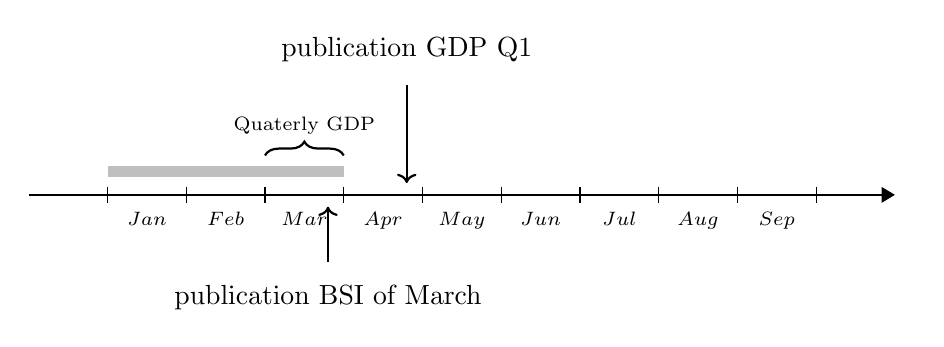
\begin{tikzpicture}
% draw horizontal line   
\draw[thick, -Triangle] (0,0) -- (\ImageWidth,0) node[font=\scriptsize,below left=3pt and -8pt]{ };

% draw vertical lines
\foreach \x in {1,...,10}
\draw (\x cm,3pt) -- (\x cm,-3pt);
\foreach \x/\descr in {1.5/Jan, 2.5/Feb, 3.5/Mar, 4.5/Apr, 5.5/May, 6.5/Jun, 7.5/Jul, 8.5/Aug,9.5/Sep}
\node[font=\scriptsize, text height=1.75ex,
text depth=.5ex] at (\x,-.3) {$\descr$};

% colored bar up
\foreach \x/\perccol in
{1/100,2/75,3/25}
\draw[lightgray, line width=4pt] 
(\x,.3) -- +(1,0);

% braces
\draw [thick ,decorate,decoration={brace,amplitude=5pt}] (3,0.5)  -- +(1,0) 
       node [black,midway,above=4pt, font=\scriptsize] {Quaterly GDP};
% time of publication
\node[align=center] at (4.8,1.85) {publication GDP Q1};
\draw [thick,->] (4.8,1.4) -- (4.8,0.15);
\node[align=center] at (3.8,-1.3) {publication BSI of March};
\draw [thick,->] (3.8,-0.85) -- (3.8,-0.15);
\end{tikzpicture}



\section{Linear Model}

\begin{eqnarray}
    YoY \text{ } GDP_{t} = \beta_0 + \sum^n_{i = 1}
       \beta_{i} X_{t} + \epsilon_t 
\end{eqnarray}

\begin{tabular}{l l}
    $GDP_t$         & GDP growth over the last semester \\
    $X_{t}$         & monthly predictors \\
    $\beta_{0}$     & constant \\
    $\beta_{i}$     & regression coefficients \\
\end{tabular}

bla bla bla

\begin{table}[H] \centering \footnotesize
  \caption{} 
  \label{} 
\begin{tabular}{@{\extracolsep{5pt}}lD{.}{.}{-3} D{.}{.}{-3} D{.}{.}{-3} D{.}{.}{-3} D{.}{.}{-3} } 
\\[-1.8ex]\hline 
\hline \\[-1.8ex] 
 & \multicolumn{5}{c}{Linear Regression} \\ 
\cline{2-6} 
\\[-1.8ex] & \multicolumn{5}{c}{Year on Year GDP (in \%)} \\ 
\\[-1.8ex] & \multicolumn{1}{c}{(1)} & \multicolumn{1}{c}{(2)} & \multicolumn{1}{c}{(3)} & \multicolumn{1}{c}{(4)} & \multicolumn{1}{c}{(5)}\\ 
\hline \\[-1.8ex] 
 Constant & 3.429^{***} & -1.740^{***} & -1.821^{***} & -1.756^{***} & -1.761^{***} \\ 
  & (0.160) & (0.631) & (0.615) & (0.635) & (0.634) \\ 
  & & & & & \\ 
 BSI & 15.773^{***} & 21.443^{***} & 21.548^{***} & 21.310^{***} & 21.116^{***} \\ 
  & (1.317) & (1.252) & (1.224) & (1.306) & (1.310) \\ 
  & & & & & \\ 
 Var(BSI) &  & 49.102^{***} & 36.477^{***} & 40.631^{***} & 39.874^{***} \\ 
  &  & (5.869) & (8.089) & (11.895) & (11.844) \\ 
  & & & & & \\ 
 EIR1 &  &  & -28.718^{**} &  &  \\ 
  &  &  & (13.792) &  &  \\ 
  & & & & & \\ 
 Var(EIR1) &  &  & 78.555^{**} &  &  \\ 
  &  &  & (35.187) &  &  \\ 
  & & & & & \\ 
 EIR2 &  &  &  & -0.709 &  \\ 
  &  &  &  & (3.878) &  \\ 
  & & & & & \\ 
 Var(EIR2) &  &  &  & 9.213 &  \\ 
  &  &  &  & (11.207) &  \\ 
  & & & & & \\ 
 EIR3 &  &  &  &  & 1.248 \\ 
  &  &  &  &  & (2.615) \\ 
  & & & & & \\ 
 Var(EIR3) &  &  &  &  & 9.944 \\ 
  &  &  &  &  & (11.141) \\ 
  & & & & & \\ 
\hline \\[-1.8ex] 
Observations & \multicolumn{1}{c}{124} & \multicolumn{1}{c}{124} & \multicolumn{1}{c}{124} & \multicolumn{1}{c}{124} & \multicolumn{1}{c}{124} \\ 
R$^{2}$ & \multicolumn{1}{c}{0.540} & \multicolumn{1}{c}{0.709} & \multicolumn{1}{c}{0.728} & \multicolumn{1}{c}{0.711} & \multicolumn{1}{c}{0.711} \\ 
Adjusted R$^{2}$ & \multicolumn{1}{c}{0.537} & \multicolumn{1}{c}{0.704} & \multicolumn{1}{c}{0.719} & \multicolumn{1}{c}{0.701} & \multicolumn{1}{c}{0.701} \\ 
Residual Std. Error & \multicolumn{1}{c}{1.112} & \multicolumn{1}{c}{0.889} & \multicolumn{1}{c}{0.866} & \multicolumn{1}{c}{0.894} & \multicolumn{1}{c}{0.893} \\ 
F Statistic & \multicolumn{1}{c}{143.463$^{***}$} & \multicolumn{1}{c}{147.283$^{***}$} & \multicolumn{1}{c}{79.773$^{***}$} & \multicolumn{1}{c}{73.079$^{***}$} & \multicolumn{1}{c}{73.247$^{***}$} \\ 
\hline 
\hline \\[-1.8ex] 
\textit{Note:}  & \multicolumn{5}{r}{$^{*}$p$<$0.1; $^{**}$p$<$0.05; $^{***}$p$<$0.01} \\ 
\end{tabular} 
\end{table} 




\section{Evaluation / Model selection}

\subsection{R-square}

\subsection{AIC and BIC}

\subsection{Mean Square Prediction Error}

\subsection{Diebold-Mariano Test}



\subsection{Out-of-Sample performances}


ME: Mean Error

RMSE: Root Mean Squared Error

MAE: Mean Absolute Error

MPE: Mean Percentage Error

MAPE: Mean Absolute Percentage Error

MASE: Mean Absolute Scaled Error

ACF1: Autocorrelation of errors at lag 1.

\section{Relative Importance}

\begin{table}[!htbp] \centering 
  \caption{} 
  \label{} 
\begin{tabular}{@{\extracolsep{5pt}} cccccccc} 
\\[-1.8ex]\hline 
\hline \\[-1.8ex] 
Z3\_sa & Z2\_sa & Z\_sa & Var\_Z2\_sa & Var\_Z3\_sa & Var\_Z\_sa & Var\_sa & E\_sa \\ 
\hline \\[-1.8ex] 
$0.010$ & $0.018$ & $0.027$ & $0.029$ & $0.039$ & $0.094$ & $0.095$ & $1.006$ \\ 
\hline \\[-1.8ex] 
\end{tabular} 
\end{table} 


\begin{table}[!htbp] \centering 
  \caption{} 
  \label{} 
\begin{tabular}{@{\extracolsep{5pt}} cccccccc} 
\\[-1.8ex]\hline 
\hline \\[-1.8ex] 
Z2\_sa & Z3\_sa & Z\_sa & Var\_Z2\_sa & Var\_Z3\_sa & Var\_sa & Var\_Z\_sa & E\_sa \\ 
\hline \\[-1.8ex] 
$-0.003$ & $-0.002$ & $0.0003$ & $0.002$ & $0.035$ & $0.038$ & $0.046$ & $0.882$ \\ 
\hline \\[-1.8ex] 
\end{tabular} 
\end{table} 



% \section{log(GDP)}


\section{Variance(X) VS Variance(Z) VS Variance(Z2)}

\section{E(Z) VS E(Z2)}


\section{Take Question 1 out of the calculation of the Indicator}

\section{until 2012 to see if variance still significant, not attrition creating effect}

\begin{landscape}
    \section{Model with before 2000 data}

\begin{table}[!htbp] \centering \footnotesize
  \caption{} 
  \label{} 
\begin{tabular}{@{\extracolsep{5pt}}lD{.}{.}{-3} D{.}{.}{-3} D{.}{.}{-3} D{.}{.}{-3} D{.}{.}{-3} D{.}{.}{-3} } 
\\[-1.8ex]\hline 
\hline \\[-1.8ex] 
 & \multicolumn{6}{c}{Linear Regression} \\ 
\cline{2-7} 
\\[-1.8ex] & \multicolumn{6}{c}{Year on Year GDP (in \%)} \\ 
\\[-1.8ex] & \multicolumn{1}{c}{(1)} & \multicolumn{1}{c}{(2)} & \multicolumn{1}{c}{(3)} & \multicolumn{1}{c}{(4)} & \multicolumn{1}{c}{(5)} & \multicolumn{1}{c}{(6)}\\ 
\hline \\[-1.8ex] 
 Constant & 3.429^{***} & -1.740^{***} & -1.821^{***} & 4.437^{***} & 0.660 & -0.519 \\ 
  & (0.160) & (0.631) & (0.615) & (0.211) & (1.899) & (2.041) \\ 
  & & & & & & \\ 
 BSI & 15.773^{***} & 21.443^{***} & 21.548^{***} & 17.374^{***} & 19.212^{***} & 20.327^{***} \\ 
  & (1.317) & (1.252) & (1.224) & (1.547) & (1.758) & (1.813) \\ 
  & & & & & & \\ 
 Var(BSI) &  & 49.102^{***} & 36.477^{***} &  & 30.545^{*} & 31.371^{**} \\ 
  &  & (5.869) & (8.089) &  & (15.269) & (14.992) \\ 
  & & & & & & \\ 
 EIR1 &  &  & -28.718^{**} &  &  & -37.120^{**} \\ 
  &  &  & (13.792) &  &  & (17.899) \\ 
  & & & & & & \\ 
 Var(EIR1) &  &  & 78.555^{**} &  &  & 53.535 \\ 
  &  &  & (35.187) &  &  & (52.433) \\ 
  & & & & & & \\ 
\hline \\[-1.8ex] 
Observations & \multicolumn{1}{c}{124} & \multicolumn{1}{c}{124} & \multicolumn{1}{c}{124} & \multicolumn{1}{c}{48} & \multicolumn{1}{c}{48} & \multicolumn{1}{c}{48} \\ 
R$^{2}$ & \multicolumn{1}{c}{0.540} & \multicolumn{1}{c}{0.709} & \multicolumn{1}{c}{0.728} & \multicolumn{1}{c}{0.733} & \multicolumn{1}{c}{0.754} & \multicolumn{1}{c}{0.779} \\ 
Adjusted R$^{2}$ & \multicolumn{1}{c}{0.537} & \multicolumn{1}{c}{0.704} & \multicolumn{1}{c}{0.719} & \multicolumn{1}{c}{0.727} & \multicolumn{1}{c}{0.744} & \multicolumn{1}{c}{0.758} \\ 
Res. Std. Error & \multicolumn{1}{c}{1.112} & \multicolumn{1}{c}{0.889} & \multicolumn{1}{c}{0.866} & \multicolumn{1}{c}{0.851} & \multicolumn{1}{c}{0.825} & \multicolumn{1}{c}{0.801} \\ 
F Statistic & \multicolumn{1}{c}{143.463$^{***}$} & \multicolumn{1}{c}{147.283$^{***}$} & \multicolumn{1}{c}{79.773$^{***}$} & \multicolumn{1}{c}{126.060$^{***}$} & \multicolumn{1}{c}{69.144$^{***}$} & \multicolumn{1}{c}{37.845$^{***}$} \\ 
\hline 
\hline \\[-1.8ex] 
\textit{Note:}  & \multicolumn{6}{r}{$^{*}$p$<$0.1; $^{**}$p$<$0.05; $^{***}$p$<$0.01} \\ 
\end{tabular} 
\end{table} 

\end{landscape}

\begin{landscape}
    \begin{table}[!htbp] \centering 
  \caption{} 
  \label{} 
\begin{tabular}{@{\extracolsep{5pt}}lD{.}{.}{-3} D{.}{.}{-3} D{.}{.}{-3} D{.}{.}{-3} D{.}{.}{-3} D{.}{.}{-3} } 
\\[-1.8ex]\hline 
\hline \\[-1.8ex] 
 & \multicolumn{6}{c}{Linear Regression} \\ 
\cline{2-7} 
\\[-1.8ex] & \multicolumn{6}{c}{Year on Year GDP (in \%)} \\ 
\\[-1.8ex] & \multicolumn{1}{c}{(1)} & \multicolumn{1}{c}{(2)} & \multicolumn{1}{c}{(3)} & \multicolumn{1}{c}{(4)} & \multicolumn{1}{c}{(5)} & \multicolumn{1}{c}{(6)}\\ 
\hline \\[-1.8ex] 
 Constant & 3.429^{***} & -1.740^{***} & -1.821^{***} & 3.903^{***} & -1.068 & -1.764 \\ 
  & (0.160) & (0.631) & (0.615) & (0.180) & (1.102) & (1.163) \\ 
  & & & & & & \\ 
 BSI & 15.773^{***} & 21.443^{***} & 21.548^{***} & 17.494^{***} & 21.469^{***} & 22.103^{***} \\ 
  & (1.317) & (1.252) & (1.224) & (1.379) & (1.518) & (1.505) \\ 
  & & & & & & \\ 
 Var(BSI) &  & 49.102^{***} & 36.477^{***} &  & 43.809^{***} & 38.891^{***} \\ 
  &  & (5.869) & (8.089) &  & (9.608) & (10.307) \\ 
  & & & & & & \\ 
 EIR1 &  &  & -28.718^{**} &  &  & -38.430^{**} \\ 
  &  &  & (13.792) &  &  & (17.020) \\ 
  & & & & & & \\ 
 Var(EIR1) &  &  & 78.555^{**} &  &  & 63.393 \\ 
  &  &  & (35.187) &  &  & (46.225) \\ 
  & & & & & & \\ 
\hline \\[-1.8ex] 
Observations & \multicolumn{1}{c}{124} & \multicolumn{1}{c}{124} & \multicolumn{1}{c}{124} & \multicolumn{1}{c}{88} & \multicolumn{1}{c}{88} & \multicolumn{1}{c}{88} \\ 
R$^{2}$ & \multicolumn{1}{c}{0.540} & \multicolumn{1}{c}{0.709} & \multicolumn{1}{c}{0.728} & \multicolumn{1}{c}{0.652} & \multicolumn{1}{c}{0.720} & \multicolumn{1}{c}{0.740} \\ 
Adjusted R$^{2}$ & \multicolumn{1}{c}{0.537} & \multicolumn{1}{c}{0.704} & \multicolumn{1}{c}{0.719} & \multicolumn{1}{c}{0.648} & \multicolumn{1}{c}{0.714} & \multicolumn{1}{c}{0.727} \\ 
Residual Std. Error & \multicolumn{1}{c}{1.112} & \multicolumn{1}{c}{0.889} & \multicolumn{1}{c}{0.866} & \multicolumn{1}{c}{1.083} & \multicolumn{1}{c}{0.977} & \multicolumn{1}{c}{0.954} \\ 
F Statistic & \multicolumn{1}{c}{143.463$^{***}$} & \multicolumn{1}{c}{147.283$^{***}$} & \multicolumn{1}{c}{79.773$^{***}$} & \multicolumn{1}{c}{161.027$^{***}$} & \multicolumn{1}{c}{109.438$^{***}$} & \multicolumn{1}{c}{58.910$^{***}$} \\ 
\hline 
\hline \\[-1.8ex] 
\textit{Note:}  & \multicolumn{6}{r}{$^{*}$p$<$0.1; $^{**}$p$<$0.05; $^{***}$p$<$0.01} \\ 
\end{tabular} 
\end{table} 
\end{landscape}{}

\chapter{Conclusion}

A large 

It was seen that


High correlation between var(BSI) and var(EIR) -> people seems to change in the same direction


\chapter{Discussion}

\section{Recruitment procedure and panel data}
not real sampling theory



\section{Z that takes more periods into account}



\section{Limitations}

\subsection*{Variance influence by drop-out, attrition, ...}

\section{Improve the business survey}

\subsubsection*{Change participants}

\subsubsection*{Mo}
From a statisticians point of view, a more sampling theory Including SRS or else would be more optimal

\subsubsection{leave question 18 out of NS975}

\section{Further Research}



More complex Nowcasting model with Space space models / MIDAS ....

Combine mixed models and Markov Chain for Panel Data \citep{de_haan-rietdijk_use_2017} 

State Space Model

Bayesian estimation \cite{bialowolski_bayesian_nodate}

%\nocite{*}
\nocite{hlavac_stargazer:_2018}
\bibliographystyle{apa}
\bibliography{references}
 


  
\begin{appendix}
  \listoffigures
  \listoftables
\end{appendix}


\chapter*{Appendix}

\section{Questions NS975}
\label{Appendix: Question NS975 description}
Questions taken into account for NS975:
....

originally question Q18, 27, 32 and 33, for simplicity numbered here as 1, 2, 3 and 4.

\subsubsection*{Verloop en beoordeling}
\begin{enumerate}
    \item Uw huidige voorraad van dit product beschouwt u, voor het seizoen, als: \\
	$\Square$	hoger dan normaal (te hoog)	$\Square$	normaal (voldoende)	$\Square$ lager dan normaal (te laag)
	
    \item Uw huidige gezamenlijke orderpositie voor dit product beschouwt u als: \\
	$\Square$ hoger dan normaal $\Square$ normaal $\Square$ lager dan normaal
\end{enumerate}

\subsubsection*{Vooruitzichten voor de volgende drie maanden} 
\begin{enumerate}
\setcounter{enumi}{2}
    \item Het personeel (arbeiders en technici) tewerkgesteld voor de fabricatie van dit product zal volgens u: \\
	$\Square$ worden uitgebreid $\Square$ onveranderd blijven $\Square$ worden verminderd
						
    \item De vraag van uw klanten naar dit product zal volgens u:  \\
	$\Square$ belangrijker $\Square$ even belangrijk $\Square$ minder belangrijk \\	
	zijn dan gewoonlijk tijdens die periode van het jaar.
\end{enumerate}

\newpage
\section*{Further Explanation of the Evolution of the responses ...}
\label{sec:appendix explanations EIR}

\begin{center}
\begin{tabular}{|c|r|r|r|}
Notation    &  $x_{t-1}$ & $x_t$ & $z_t$ \\\hline
$\pi_{--}$    &  -1  & -1    & 0 \\
$\pi_{-0}$    &  -1  & 0     & 1 \\
$\pi_{-+}$    &  -1  & 1     & 2 \\
$\pi_{0-}$    &  0   & -1    & -1 \\
$\pi_{00}$    &  0   & 0     & 0 \\
$\pi_{0+}$    &  0   & 1     & 1 \\
$\pi_{+-}$    &  1   & -1    & -2 \\
$\pi_{+0}$    &  1   & 0     & -1 \\
$\pi_{++}$    &  1   & 1     & 0 \\
\end{tabular}  
\end{center}

\newpage

\section*{Test for seasonality}
\label{sec:test for seasonality}

\newpage
\section*{Further Explanation of the Markov Switching model ...}


\newpage
\begin{figure}[H]
    \centering
%    \captionsetup{justification=centering}
    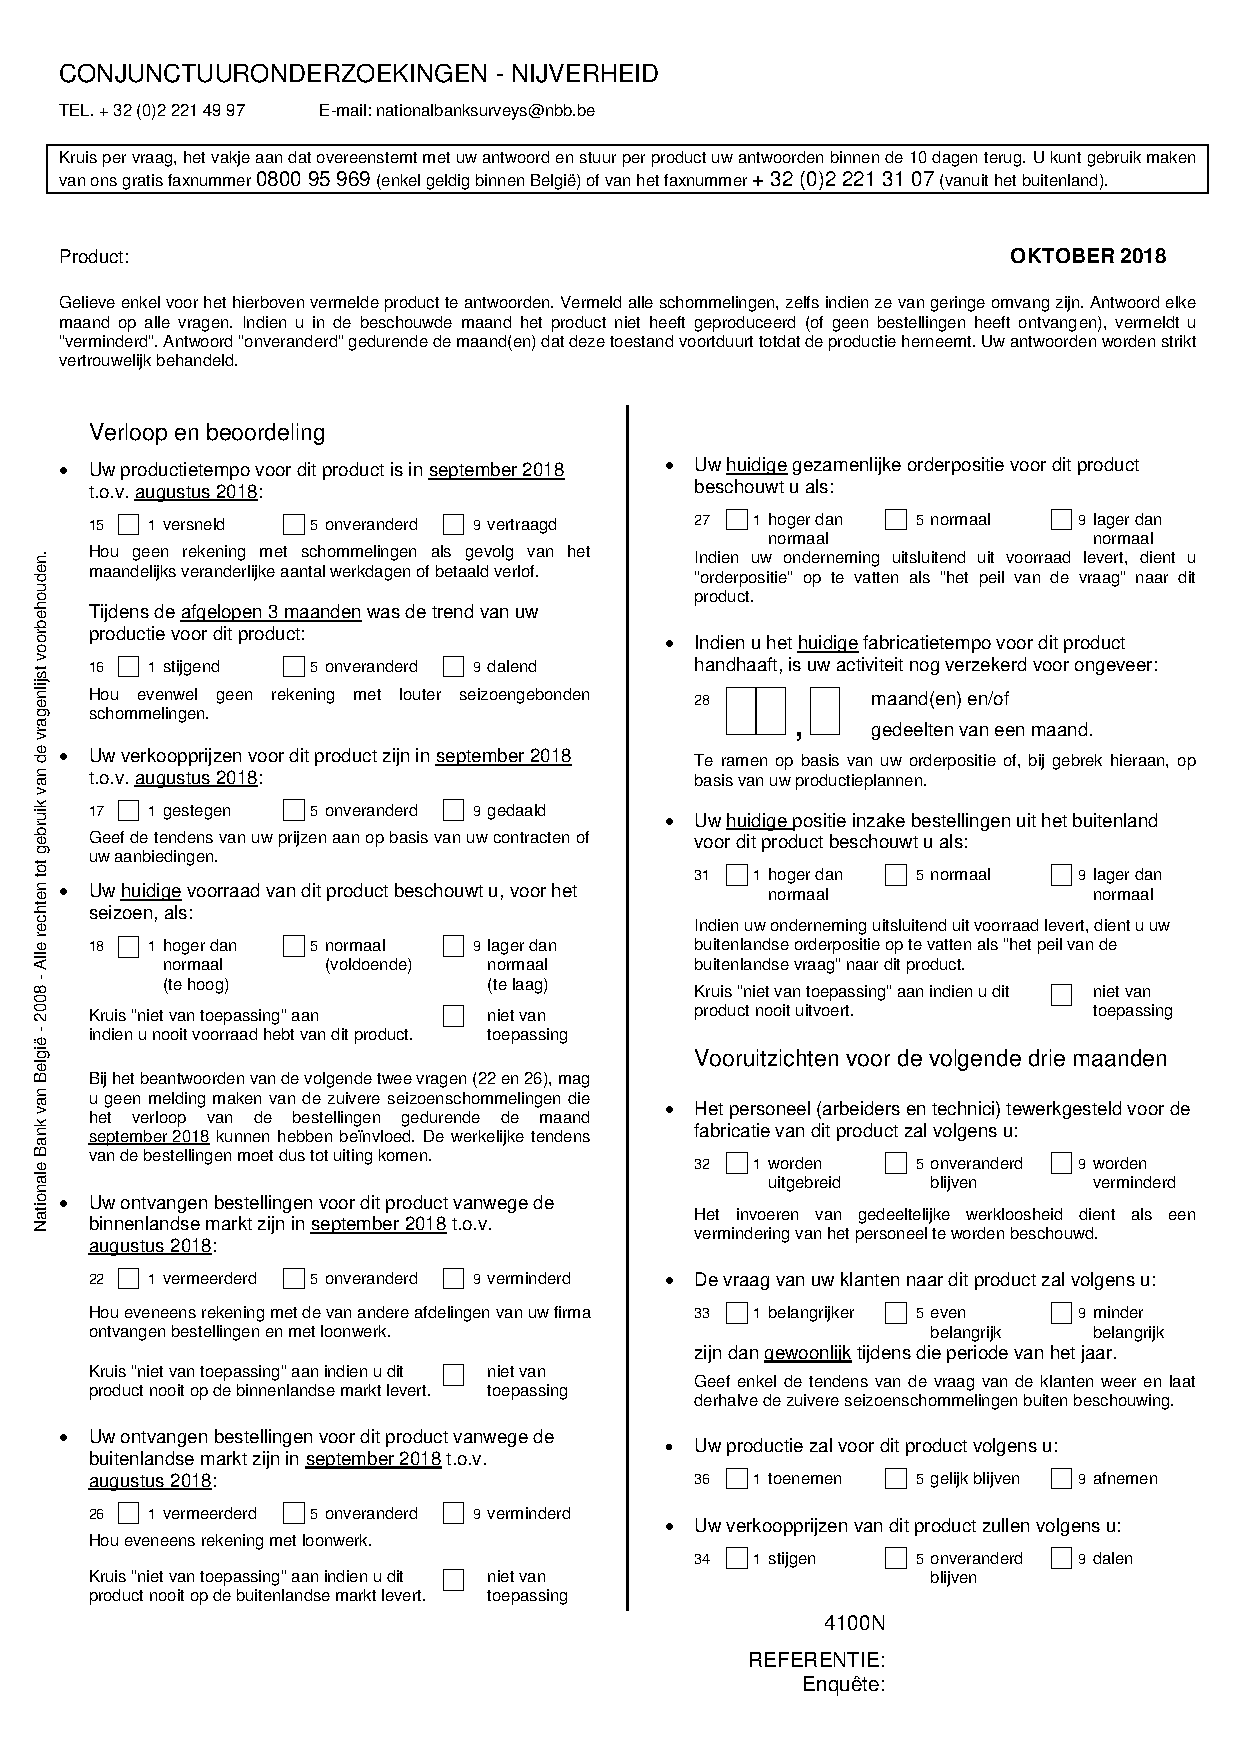
\includegraphics[scale=0.75]{Images/IndustryN.pdf}
    \caption{The Business Survey Questionnaire in Dutch for the Industrial Sector in 2018}
    \label{Questionnaire2018}
\end{figure}

\begin{figure}[H]
    \centering
%    \captionsetup{justification=centering}
    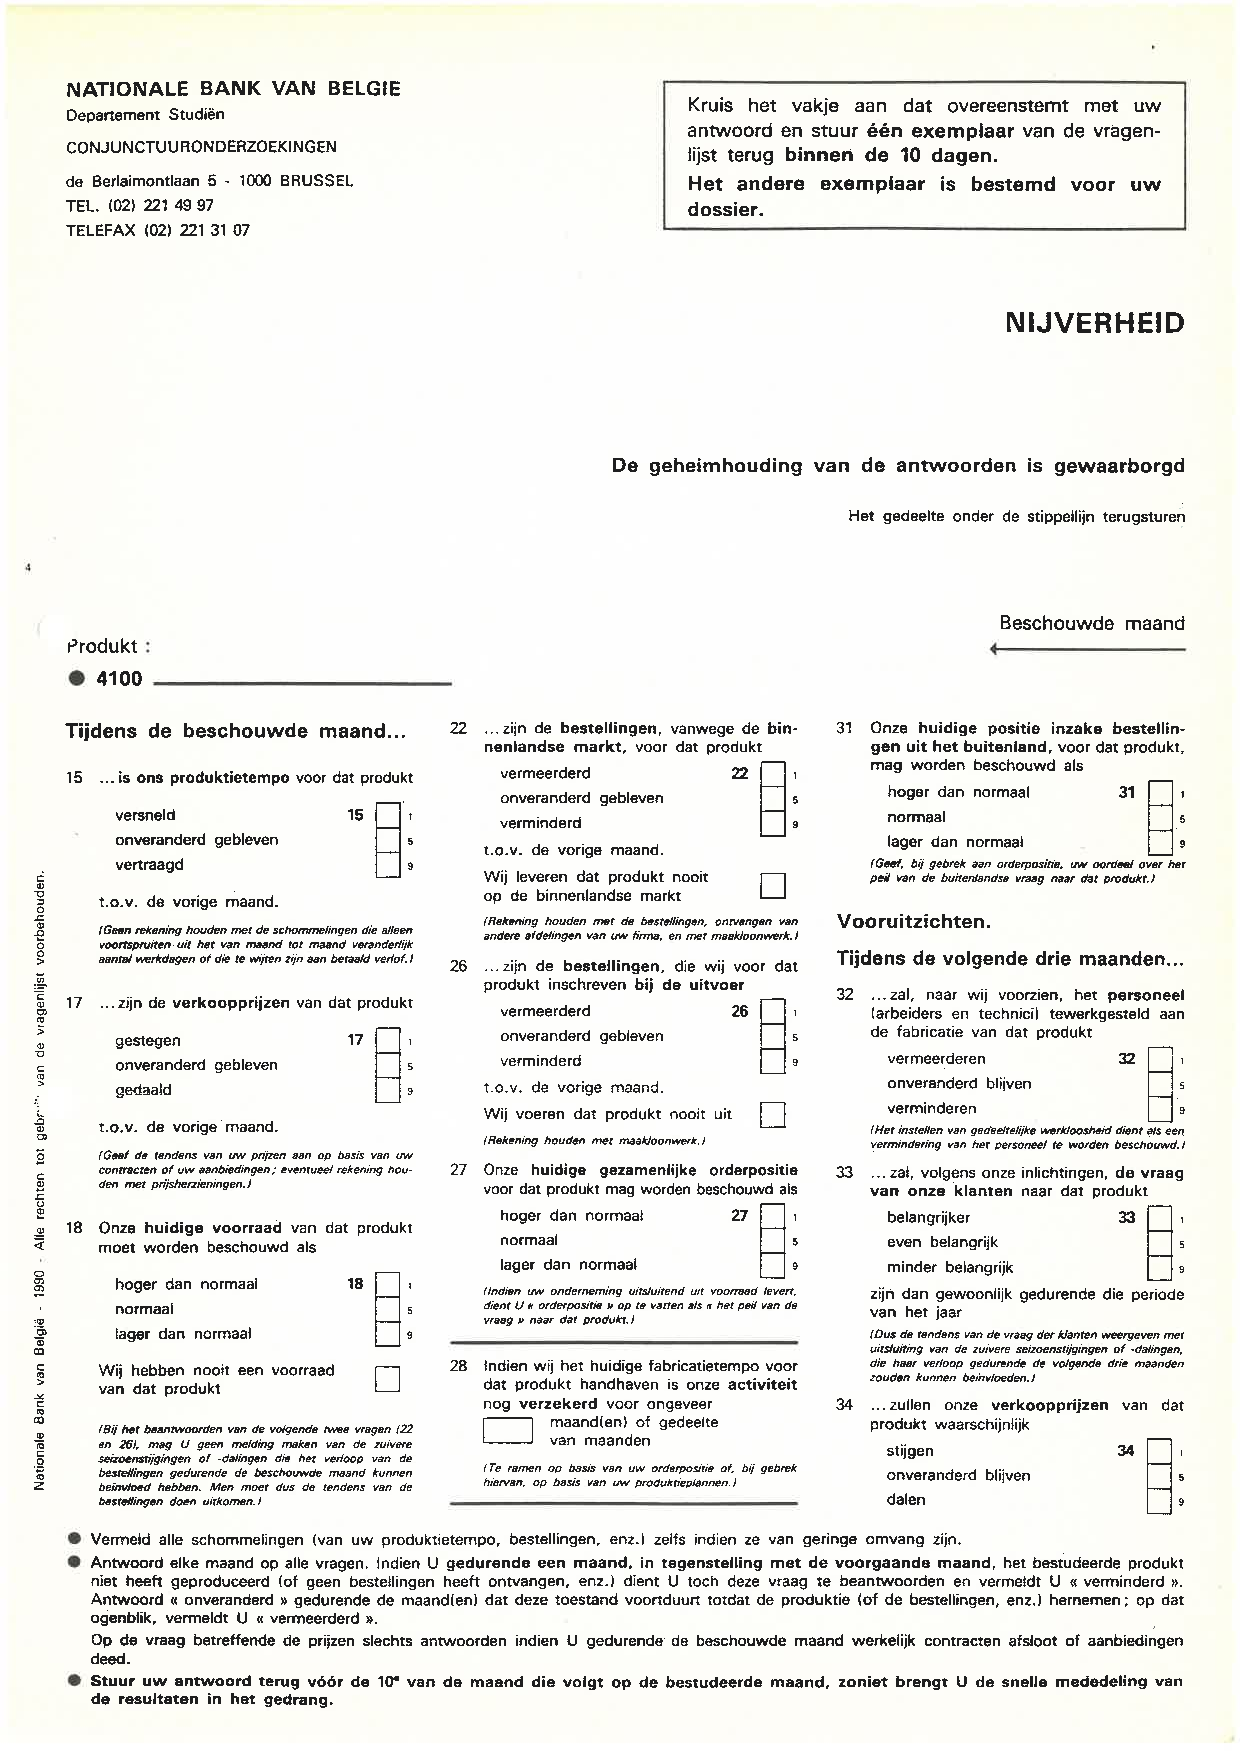
\includegraphics[scale=0.75]{Images/4100N_v1990.pdf}
    \caption{The Business Survey Questionnaire in Dutch for the Industrial Sector in 1990}
    \label{Questionnaire1990}
\end{figure}


\begin{figure}[H]
    \centering
    \captionsetup{justification=centering}
    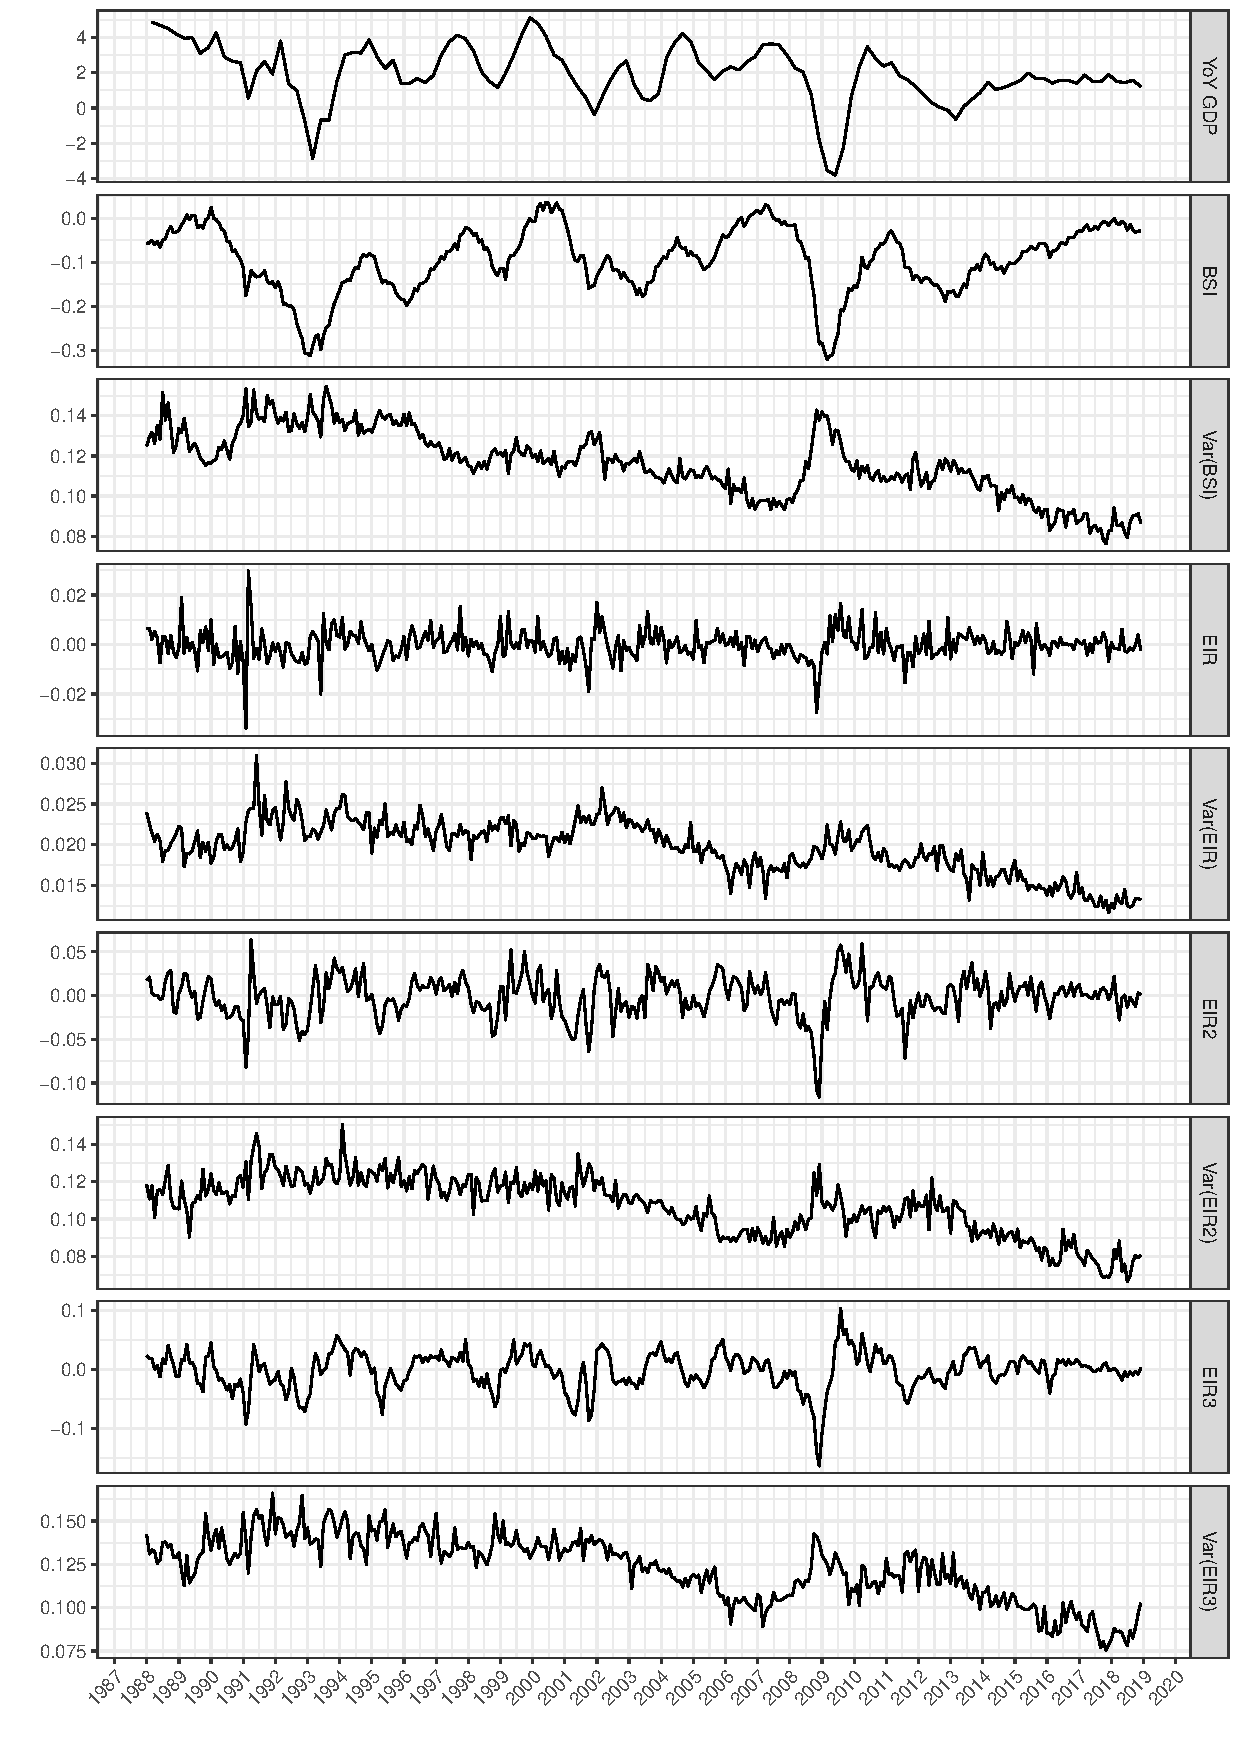
\includegraphics[scale=0.8]{Graphs/variables.pdf}
    \caption{Plot }
    \label{plot:appendix all variables}
\end{figure}


\chapter*{Code}
\section*{R code for Seasonal Adjustment}


\section*{R code for Creating Lags}


\section*{R code for Linear (Auto-Regressive) Models}

\href{https://github.com/fabricevb/Master-Thesis/blob/master/R%20Code/Linear%20Regression.R}{Code for Linear Models on https://github.com/fabricevb/Master-Thesis}


\section*{R code for Markov Switching Models}

\newpage

% ----------------------- Back cover ------------------------------
% Please fill in:
% - Department
% - Department's address
% - Telephone number and fax number
% -----------------------------------------------------------------
\thispagestyle{empty}
\sffamily
%
\begin{textblock}{191}(113,-11)
{\color{blueline}\rule{160pt}{5.5pt}}
\end{textblock}
%
\begin{textblock}{191}(168,-11)
{\color{blueline}\rule{5.5pt}{59pt}}
\end{textblock}
%
\begin{textblock}{183}(-24,-11)
\textblockcolour{}
\flushright
\fontsize{7}{7.5}\selectfont
\textbf{AFDELING}\\
Straat nr bus 0000\\
3000 LEUVEN, BELGI\"{E}\\
tel. + 32 16 00 00 00\\
fax + 32 16 00 00 00\\
www.kuleuven.be\\
\end{textblock}
%
\begin{textblock}{191}(154,-7)
\textblockcolour{}
\includegraphics*[height=16.5truemm]{Images/sedes}
\end{textblock}
%
\begin{textblock}{191}(-20,235)
{\color{bluetitle}\rule{544pt}{55pt}}
\end{textblock}















\end{document}
